\documentclass[aps,%
12pt,%
final,%
oneside,
onecolumn,%
superscriptaddress,%
centertags]{article} %%
\topmargin=10em
\textheight=600pt
\usepackage[english]{babel}
\usepackage[utf8]{inputenc}
\usepackage[colorlinks=true,urlcolor=black,linkcolor=black,filecolor=black,citecolor=black,unicode,pdftex]{hyperref}
%\usepackage{supertabular}
\usepackage[pdftex]{graphicx}
%\usepackage{amsthm,amssymb, amsmath}
%\usepackage{textcomp}
%\usepackage[noend]{algorithmic}
%\usepackage[ruled]{algorithm}
\selectlanguage{english}

\begin{document}

\begin{titlepage}
\begin{center}

% Title
\textbf{\LARGE Git – Subversion Translation} \\[1.0cm]
\textbf{\LARGE Specification} \\[3.0cm]

\textbf{Alexander Kitaev} \\[0.7cm]
\textbf{Dmitry Pavlenko} \\[0.7cm]
\textbf{Marc Strapetz} \\[0.7cm]
\textbf{Semen Vadishev} \\[0.7cm]

\end{center}
\end{titlepage}

\topmargin=-10pt
\setcounter{page}{2}

\newpage
\hrule
\tableofcontents

\newpage
\hrule
\section{Translator Architecture}
\subsection{Translator Components}
\renewcommand{\figurename}{Figure}

Translator runs as a separate component independent on existing GitHub infrastructure. Translator is responsible for:
\begin{itemize}
  \item Translating existing Git Commits to Subversion revisions
  \item Processing of Subversion user's requests
  \item Translating new Subversion revisions to Git commits
  \item Pushing translated Git commits to GitHub Git repository
\end{itemize}
Translator components are depicted on the diagram \ref{translator_components_pic}:
\begin{center}
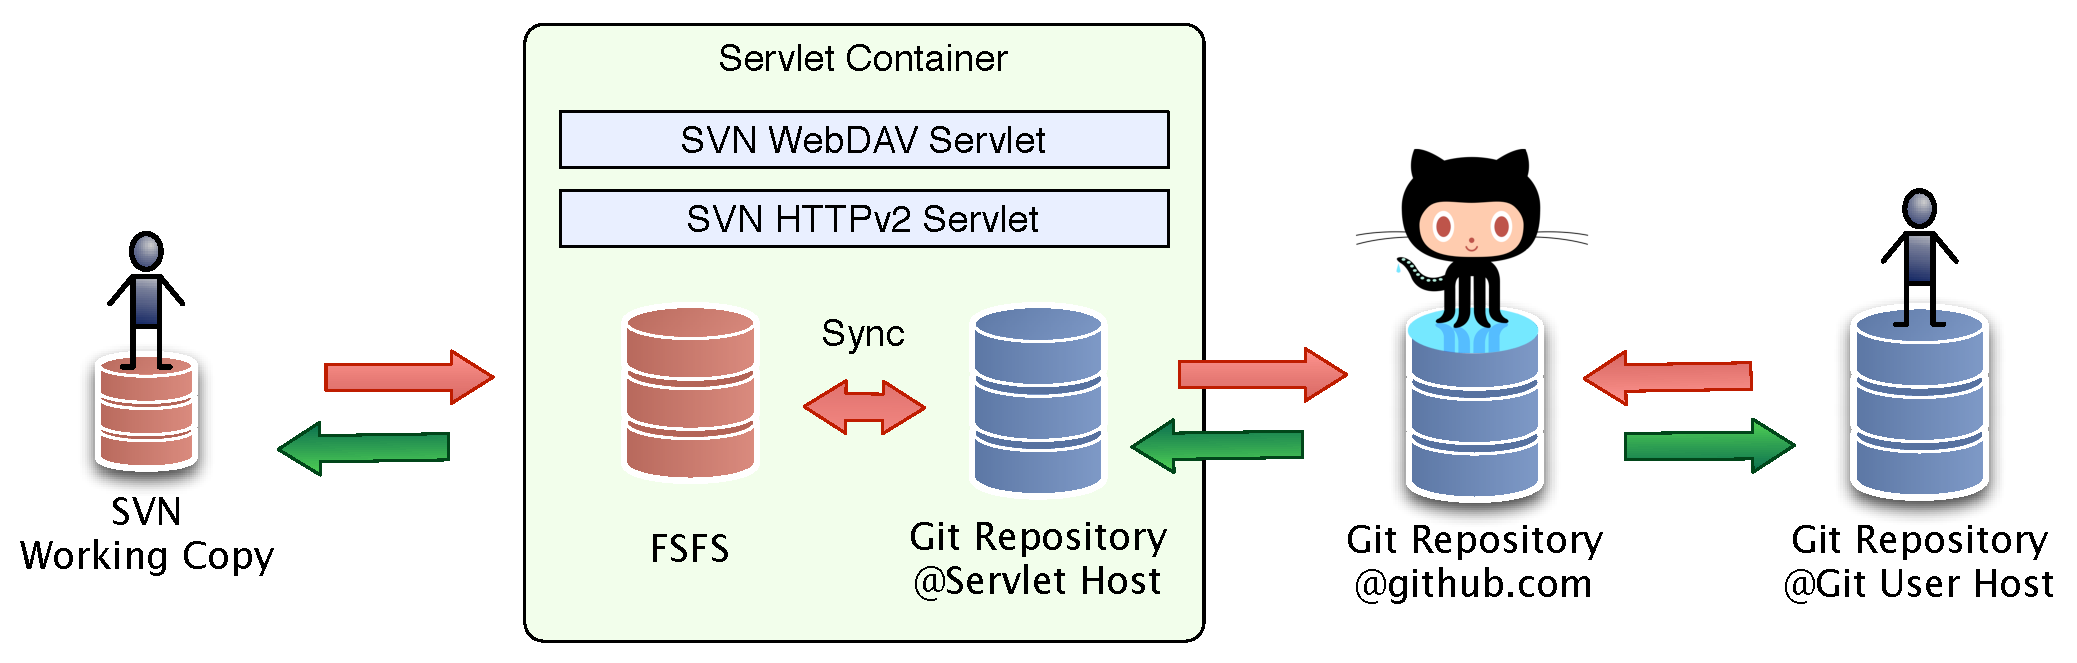
\includegraphics[width=\textwidth]{img/servlet/components_keep_github_safe.pdf}%
\captionof{figure}{Translator Components.}
\label{translator_components_pic}%
\end{center}

Translator major features from the architecture perspective are \emph{maximum level of reuse} of the standard existing components, and \emph{minimum interference} with the existing GitHub infrastructure. 
Let's take a look at how these features are implemented. This chapter provides an overview of Translator components and further chapters provides more details on how each particular operation is carried on.

\label{srp}
\subsubsection{Subversion Requests Processor}
In order to process Subversion user's requests sent over HTTP protocol, Translator is implemented as a Java servlet which might be ran inside any servlet container. All Subversion requests are served by the standard Subversion processing code which serves 
these request by reading from or writing to the local Subversion repository (see FSFS at figure \ref{translator_components_pic}).
\\\\
Processing some of the write requests includes calls to \emph{hooks} which instantly translates Subversion revisions to Git commits.
These \emph{hooks} should not be mixed up with the standard Subversion post- and pre- commit hooks. 
Here the hooks injected into Subversion code by Translator are meant.\\\\
While Subversion commit algorithm remains unmodified, it makes calls to the Translator code at certain strategic points, 
and to these calls we refer as to \emph{hooks} here.
\\\\
\textbf{Reused:} existing Subversion codebase;\\Subversion repository as a data storage.\\
\textbf{Interference with GitHub infrastructure:} none. 

\subsubsection{Git to Subversion Translator}
To make any sense, local Subversion repository must be kept up to date with its GitHub counterpart, i.e. it has to include all the changes committed into GitHub repository by Git users. Synchronization of the local Subversion repository with GitHub Git repository is performed in two steps:
\begin{enumerate}
\compactlist
\item Changes in GitHub Git repository are pulled to the local Git repository
\item Git commits from local Git repository are imported into the local Subversion repository
\end{enumerate} 
Synchronization takes place:
\begin{itemize}
\item Before Subversion repository becomes available to the users, to import existing Git commits into Subversion repository
\item Just before Subversion commit is translated into Git commit to make sure Subversion repository is up to date
\item On schedule, to minimize delays on commit
\end{itemize}
Sychronization must be peformed at commit time. As long as there are only read requests 
to Subversion repository, there might be a delay in synchronization so that new Git
commits are imported into Subversion repository in the time most convenient from the 
load balance perspective.
\\\\
Import of Git commits into Subversion repository is performed with the help of SVNGitKit Java library.
\\\\
\textbf{Reused:} SVNGitKit library to import commits; Git code to clone and fetch from GitHub Git repository into the local one.\\
\textbf{Interference with GitHub infrastructure:} similar to other GitHub clients, this component of Translator clones and then fetches new changes into its clone of GitHub repository.

\subsubsection{Subversion to Git Translator}
Commits made by Subversion users are instantly translated into Git commits which are then pushed into GitHub Git repository. Component responsible 
for that instant translation and push is implemented as \emph{hooks} called by Subversion code during commit (see \ref{srp}).
\newpage 
This approach helps to make sure that Subversion commit and corresponding Git push operation are part of the same transaction and either succeeds or fails together.
For more detailed description of how Subversion commits are processed, refer to the section 1.2 of this specification.
\\\\
\textbf{Reused:} Instant translation uses SVNGitKit library, small part of the code is custom, in particular part which is responsible for integrity of Subversion commit and Git push pair.\\
\textbf{Interference with GitHub infrastructure:} similar to other GitHub clients, this component of Translator performs push of the new Git objects into GitHub Git repository. 

\subsubsection{GitHub Integration}

Translator architecture minimizes interference with the existing GitHub infrastructure which is clearly an advantage, but there is a performance penalty being paid for that.
In particular, there is synchronization of the local Git repository with the GitHub Git repository using fetch and push operations. Moreover, both fetch and push are 
performed as part of Subversion commit operation, which might make Subversion commits slow and prone to timeout related errors.
\\\\
To resolve this potential performance issue, Translator could benefit from having local filesystem access to the GitHub repository. Then Translator may work directly with GitHub repository,
with no need to use expensive push and fetch operations.
\begin{center}
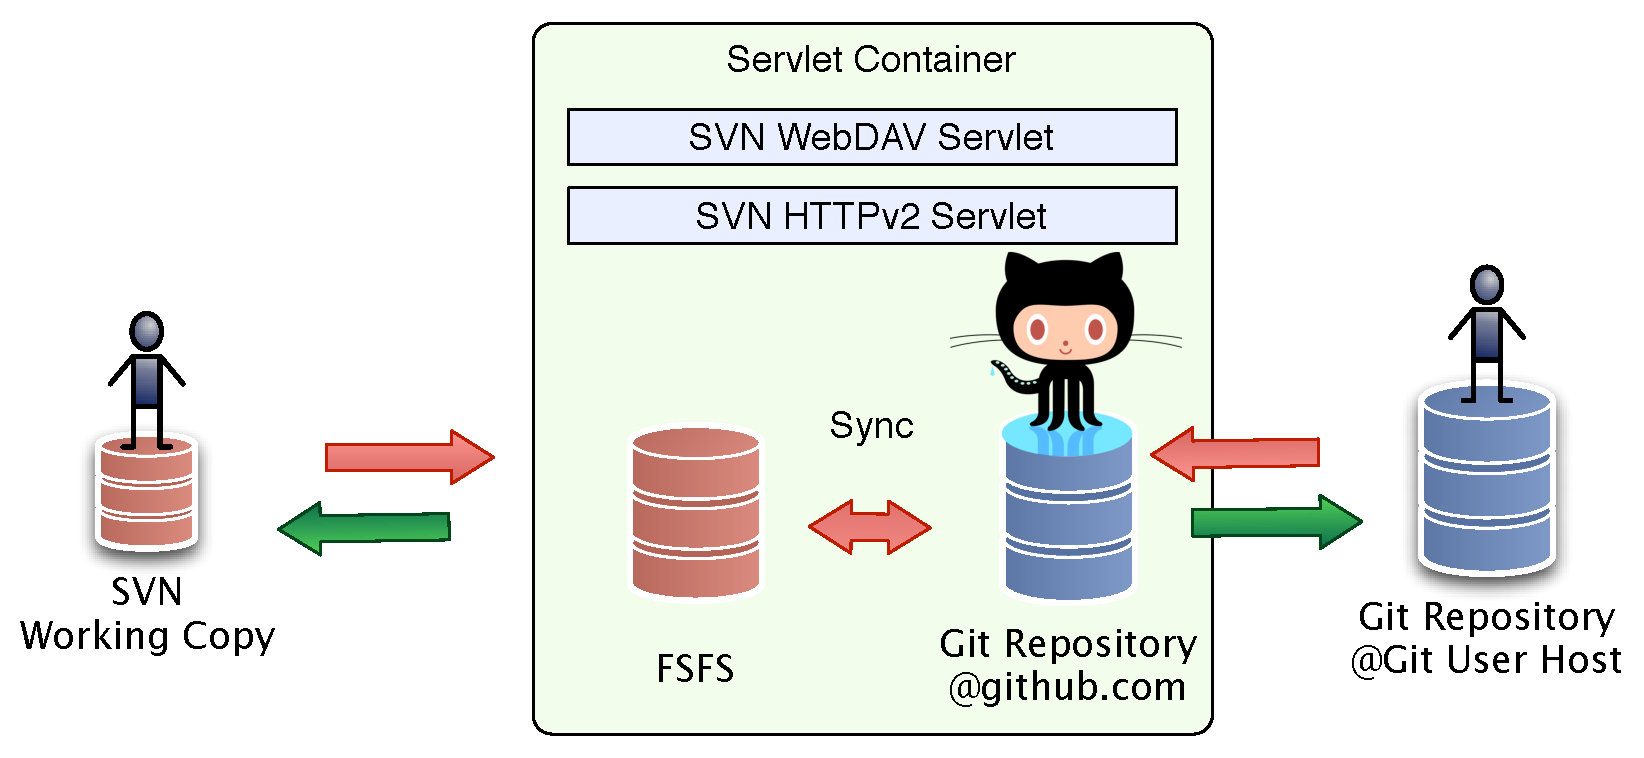
\includegraphics[width=\textwidth]{img/servlet/components_not_that_safe.pdf}%
\captionof{figure}{Higher level of interference.}
\label{translator_components_pic2}%
\end{center}

Major drawback of that solution is that theoretically, bug in Translator code may damage existing GitHub repository contents.
\subsection{Commits to Revisions Mapping}

Translator performs translation of Git commits created by Git users into Subversion revisions, as well
as mirror translation of Subversion revisions created by Subversion users into Git commits. This section
describes how one concept (revision or commit) is mapped into another by Translator and how this mapping 
is stored.

\subsubsection{Git Commits to Subversion Revisions}

Every Git commit is translated to a single Subversion revision which modifies (or creates) a single branch or tag
in Subversion repository. Some of the non-commit changes, like Git branch or tag object creation are also translated into Subversion revisions.\\\\
\begin{figure}[!h]
\centering
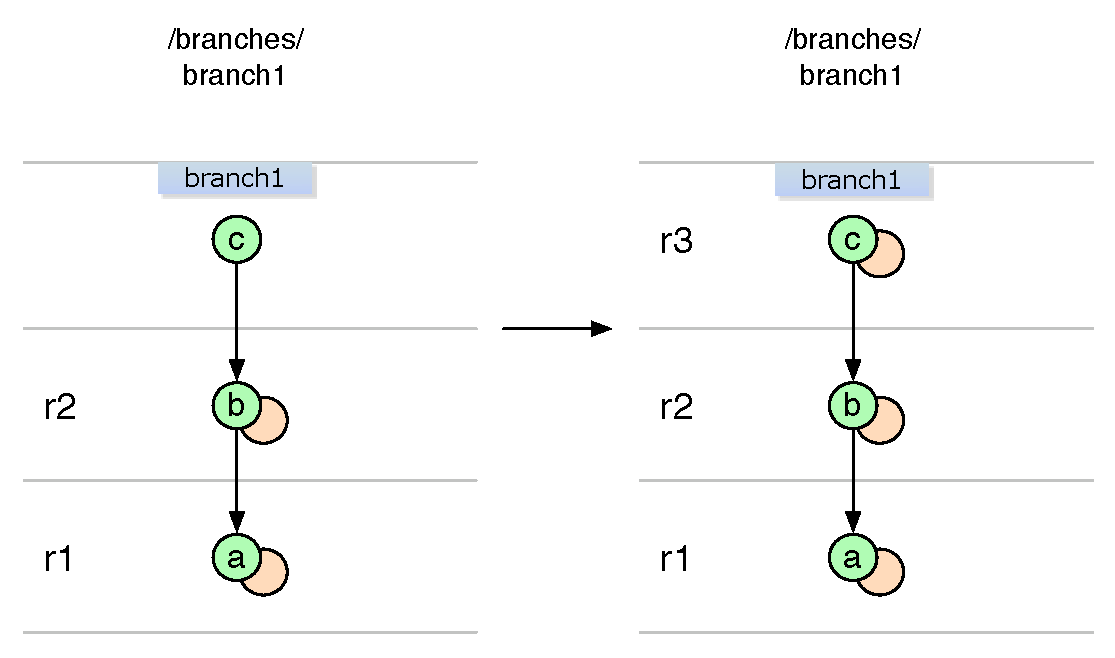
\includegraphics[width=\linewidth]{img/diagrams/single_change_git_to_svn.pdf}
\caption{Git Commit being translated to Subversion Revision}
\label{simple_git_to_svn}
\end{figure}Mapping between Git commit objects and corresponding revisions in Subversion repository (pair of revision number and branch name) is 
kept in Git repository, in a way similar to the one used to store Git notes. 
\\\\
Translator creates a special branch named /refs/mapping/svn and creates files in this branch named with Git commit object Id - this is the first part of the mapping. % S.: Not branch, but reference. Branch is something like /refs/heads/master or /refs/remote/origin/master.%
Contents of the file is Subversion revision number and branch name - second part of the mapping.
\\\\ 
By merging contents /.git/refs/mapping/svn branch to /.git/refs/notes we will get user friendly output of the mapping as part of the standard git log.

\subsubsection{Subversion Revisions to Git Commits}

Every Subversion revision is translated into one or more Git commits, depending on the amount of the branches affected by that particular Subversion commit.\\\\% S.: Maybe add a link to Branch and Tags subsection where all that stuff is considered? Maybe move all the diagrams from that section to the following one? And here just put references to them?%
Mapping between Subversion revision and corresponding Git commits is kept in Subversion repository in form of a special revision property.
\begin{figure}[!h]
\centering
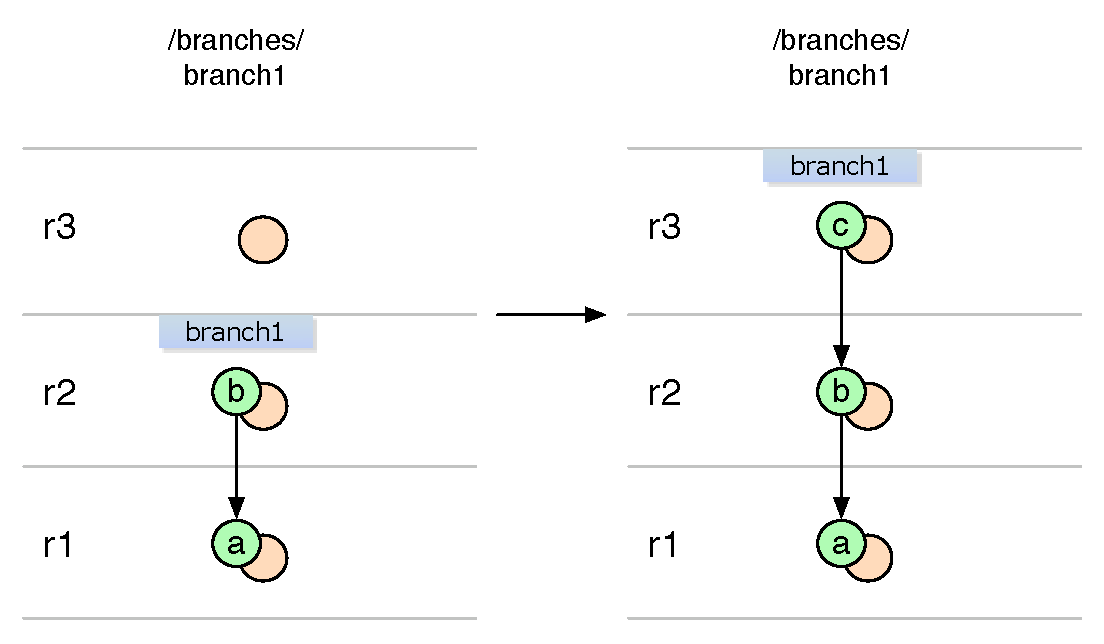
\includegraphics[width=\linewidth]{img/diagrams/single_change_svn_to_git.pdf}
\caption{Subversion Revision being translated to Git Commit}
\label{simple_svn_to_git}
\end{figure}
\\\\
Both mappings are kept in corresponding repositories (in a special branch and as revision properties), so that no special storage is needed. 
These mappings are available to the standard Git and Subversion clients.
\subsection{Processing Subversion Commits}

Translator plugs into the standard Subversion commit process so, that after Subversion commit operation
is completed and new revision is visible to Subversion user, Translator guarantees that translated Git commits
corresponding to this very revision are available to GitHub Git repository users.
\\\\
Thus, Translator guaranties atomicity and integrity of the transaction composed of Subversion commit operation
and Git commit creation and push.
\\\\
Subversion handles user's commit request in the following way:

\begin{enumerate}
\compactlist
\item Commit transaction is constructed from user's description of it. Multiple transactions might be constructed simultaneously.
\item \textbf{Hook 1} is executed.
\item \textbf{Hook 2} is executed. Commit transaction is then "merged" with the latest repository revision. In case there is a conflict (file modified by transaction might be modified by another transaction already), then out-of-date error is reported and commit is aborted. Otherwise transaction is assigned a base revision.
\item Repository is locked for writing (using file system lock) and in scope of this lock, transaction is converted to the immutable repository revision. In case transaction base revision differs from the actual latest repository revision (which is verified very early), then repository is unlocked and another attempt to merge transaction and reassign base revision to it is performed (go to 2).
\item \textbf{Hook 3} is exectued. Repository latest revision (visible to the users) is updated atomically and repository is unlocked.
\end{enumerate}
To perform instant translation and push, Translator plugs into \textbf{Hook 1}, \textbf{Hook 2} and \textbf{Hook 3} points of the commit handling process.
\\\\
\textbf{Hook 1:} Local Git repository synchronized with its GitHub origin. Local Subversion repository is synchronized with the local Git repository.
\\\\
\textbf{Hook 2:} Git Commit objects are created, Git braches and tags modified accordingly to the translation rules.
\\\\
\textbf{Hook 3:} Local Git repository changes are pushed to GitHub origin repository.
\\\\
This way, unless Subversion commit succeeded, no Git translation and push will take place and unless push have succeeded, new Subversion revision will not become visible.

\subsection{Processing Git Commits}
\subsection{Fixed Subversion Repository Layout}

To support sane translation of Git branches and tags concepts into corresponding Subversion concepts, Translator must enforce certain Subversion repository layout and introduce limitations which are not present in the standard Subversion repository. 
In practice, these limitations will have no or very limited influence on real Subversion use cases.
\\\\
\textbf{Layout:}\\ 
Subversion repository always has the following directories:
\\\\
/trunk\\
/branches\\
/tags\\\\
\textbf{Limitations:}
\begin{enumerate}
\compactlist
\item no directories or files may be created in the root of repository
\item /branches and /tags directories may not be deleted or copied, /trunk may not be deleted
\item /branches/\emph{B} directory may only be created as a copy of /trunk or
as a copy of another /branches/\emph{A} or /tags/\emph{T} directory
\item /tags/\emph{T} directory may only be created as a copy of /trunk or
as a copy of another /tags/\emph{A} or /branches/\emph{B} directory
\item no directory except of direct children of /tags or /branches might be a
copy of /trunk or of /tags/\emph{T} or of /branches/\emph{B} directory
\item no files might be created in /tags and in /branches directories
\end{enumerate}
Above layout and listed limitations corresponds exactly to the Subversion common practice informal standard which
is used in case when Subversion repository contains a single project. Subversion does not encourage people 
to keep multiple projects in the same repository, but some users may prefer the following layout:
\\\\
/projectX/trunk\\
/projectX/branches\\
/projectX/tags\\
/projectZ/trunk\\
/projectZ/branches\\
/projectZ/tags\\\\
or any other combination of the standard layout components and project or subsystem names. Translator does not support such layouts as they 
makes sane branches and tags concepts translation more complicated and ambiguous.

\section{Translated Concepts}
\subsection{Subversion Branches and Tags}
\label{section_branches_and_tags}
\renewcommand{\figurename}{Diagram}

Creation, deletion or replacement of any of the Subversion /branches/\emph{branch} or /tags/\emph{tag} directory
is translated into creation, deletion or replacement of the corresponding Git reference object (Git tag or branch). 
\\\\
Depending on the absence or presence of the actual contents modification accompanying creation of the /branches/\emph{branch} 
or /tags/\emph{tag} directory, translation may or may not result in a Git commit creation, additionally 
to the reference object creation.
\\\\
There is no technically enforced difference between Subversion branches and tags. Translator, however, translates
/branches/\emph{branch} directories into Git branch references and /tags/\emph{tag} directories into Git tag objects.
Thus there are no differences in translation of Subversion branches and tags, except for those outlined below:
\begin{enumerate}
	\compactlist
	\item On creation
	\begin{itemize}
		\item Creation of /branches/\emph{B} directory leads to creation of a new branch reference \emph{B}.
		\item Creation of /tags/\emph{T} directory leads to addition of corresponding Tag Object with name \emph{T}.
	\end{itemize}
	\item On modification
	\begin{itemize}
		\item Modification which affects paths in /branches/\emph{B} directory leads to updating of corresponding branch reference \emph{B}.
		\item Modification which affects paths in /tags/\emph{T} directory leads to the removal of obsolete Tag Object with name \emph{T} and creation of new Tag Object with the same name \emph{T} for corresponding Commit Object.
	\end{itemize}
	\item On removal
	\begin{itemize}
		\item Removal of /branches/\emph{B} directory leads to removal of corresponding reference \emph{B} at Git repository.
		\item Removal of /tags/\emph{T} directory leads to removal of corresponding Tag Object with name \emph{T}.
	\end{itemize}
\end{enumerate}
Further scenarios specifies translation rules for Subversion branches, but are applicable for Subversion tags as well, 
with the differences outlined above being taken into account.
%\\\\
%The same rules could be treated in opposite direction --- every change of Git branch or tag leads to corresponding change of Subversion branch or tag.
%\\\\
%This and further chapters consider scenarios with branches only. Every scenario could be applied to tags with the rules above taken into account.
%\\\\
%Basically Translator tracks all the references located at Git repository and synchronizes every such reference with certain Subversion branch. The exact way of this synchronization described further.

\subsubsection{Subversion Branch Creation}

For the purpose of this specification, Subversion branch is a subdirectory in the top-level /branches directory of
Subversion repository. Name of that very subdirectory is a branch name. /trunk top-level directory is considered to be a branch named \emph{master}.
/trunk branch always exists in Subversion repository. Other branches might be created in different ways and thus there are 
multiple ways to translate branch creation.
\\\\
1. Most common way to create a Subversion branch is to make a copy of another branch at particular revision.
Diagram \ref{branch_creation_svn_to_git} depicts translation of a new Subversion branch \emph{/branches/branch2} created 
at revision r3 into creation of a Git commit \emph{c} and creation of a Git branch reference \emph{branch2}. Relationship 
between \emph{/branches/branch2} and \emph{/branches/branch1} is translated into a child-parent reference between new commit \emph{c} and commit \emph{b}.
\begin{center}
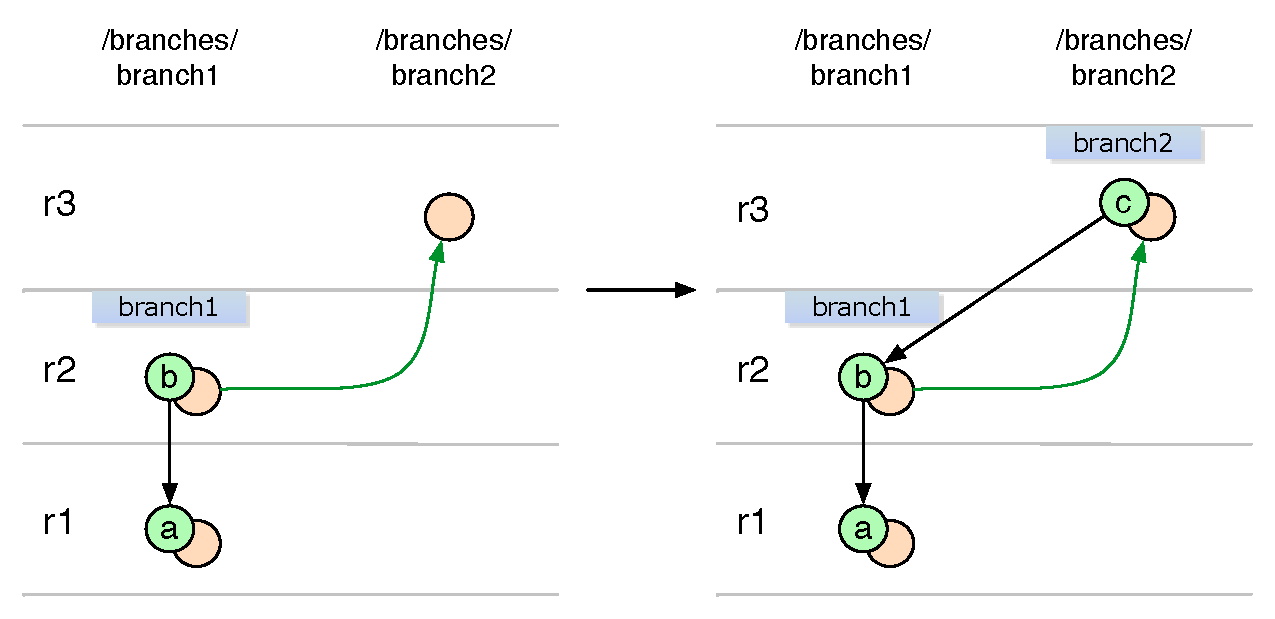
\includegraphics[width=\textwidth]{img/diagrams/branch_creation_svn_to_git.pdf}%
\captionof{figure}{Subversion branch copy being translated to Git branch creation.}
\label{branch_creation_svn_to_git}%
\end{center}
New Git commit \emph{c} contents might or might not be different from that of the Git commit \emph{b}. 
This depends on whether Subversion branch creation included content modification or not. New Git commit
\emph{c} preserves metadata of Subversion revision 3, in particular author, commit message and commit date.
\\\\
2. Another, less common way to create a branch in Subversion is to create new directory in /branches top-level
folder and then merge changes made on another branch into the newly created directory. This way
establishes relationship between new and original branch with the help of merge tracking information.
\\\\
Diagram \ref{branch_creation_from_mergeinfo_svn_to_git} demonstrates how this kind of branch origin 
is translated into the child-parent reference between new and previous commit, just like in the 
case of branch created by copying.
\begin{center}
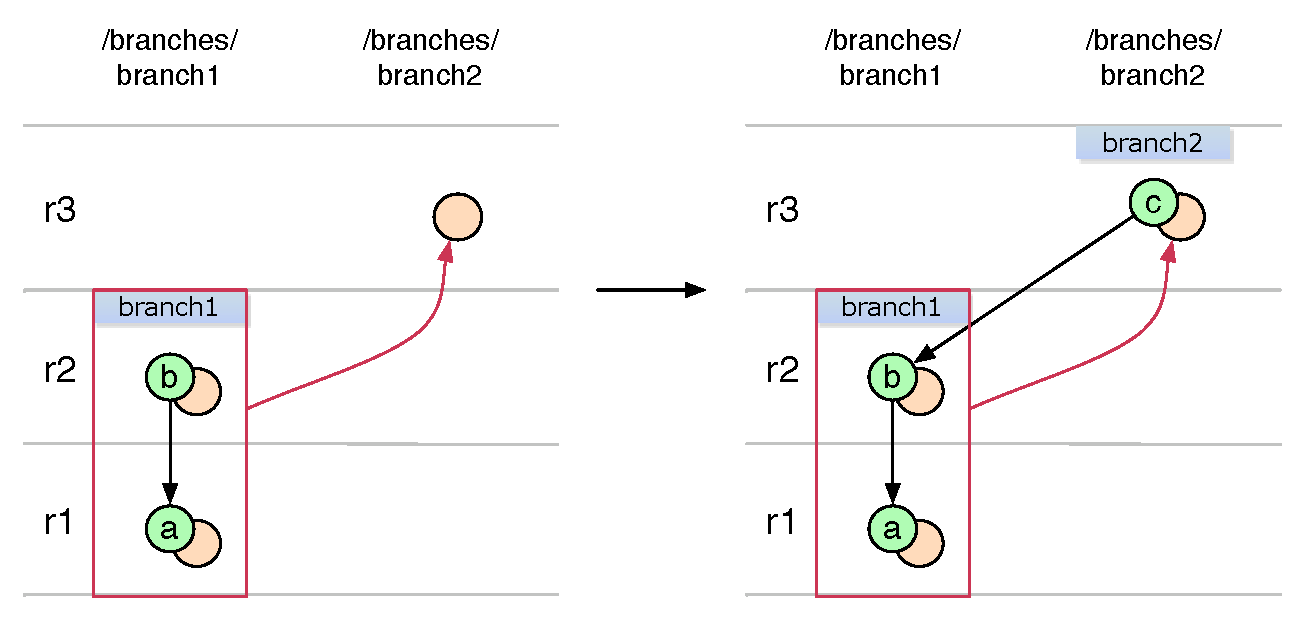
\includegraphics[width=\textwidth]{img/diagrams/branch_creation_from_mergeinfo_svn_to_git.pdf}%
\captionof{figure}{Subversion branch addition with merge history being translated to Git branch creation.}
\label{branch_creation_from_mergeinfo_svn_to_git}%
\end{center}

3. Finally, branch might be created with an empty history, i.e. with no reference to any of the existing 
revisions. In this case, as shown on the diagram \ref{branch_creation_no_history_svn_to_git} no child-parent
reference is created for the new Git commit \emph{c}. 

\begin{center}
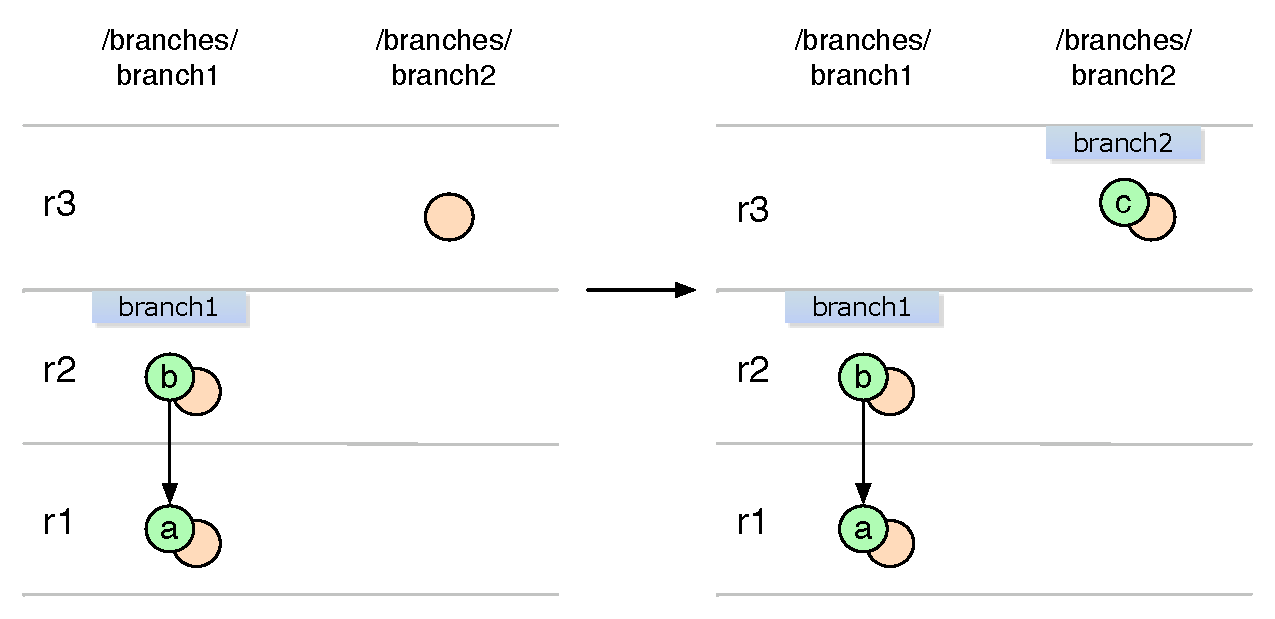
\includegraphics[width=\textwidth]{img/diagrams/branch_creation_no_history_svn_to_git.pdf}%
\captionof{figure}{Subversion branch addition with no history being translated to creation of Git branch referenced to commit with no parents.}
\label{branch_creation_no_history_svn_to_git}%
\end{center}

\subsubsection{Modification on Subversion Branch}

As already specified in the previous section (see \ref{section_revisions_and_commits}), Subversion
revision is translated into multiple Git commits - one Git commit for each group of 
affected paths, paths being grouped by the branch they belong to.
\\\\
See diagram \ref{double_branch_change_svn_to_git} for an example of multiple commits 
on different Git branches being created for a single Subversion revision.

\begin{center}
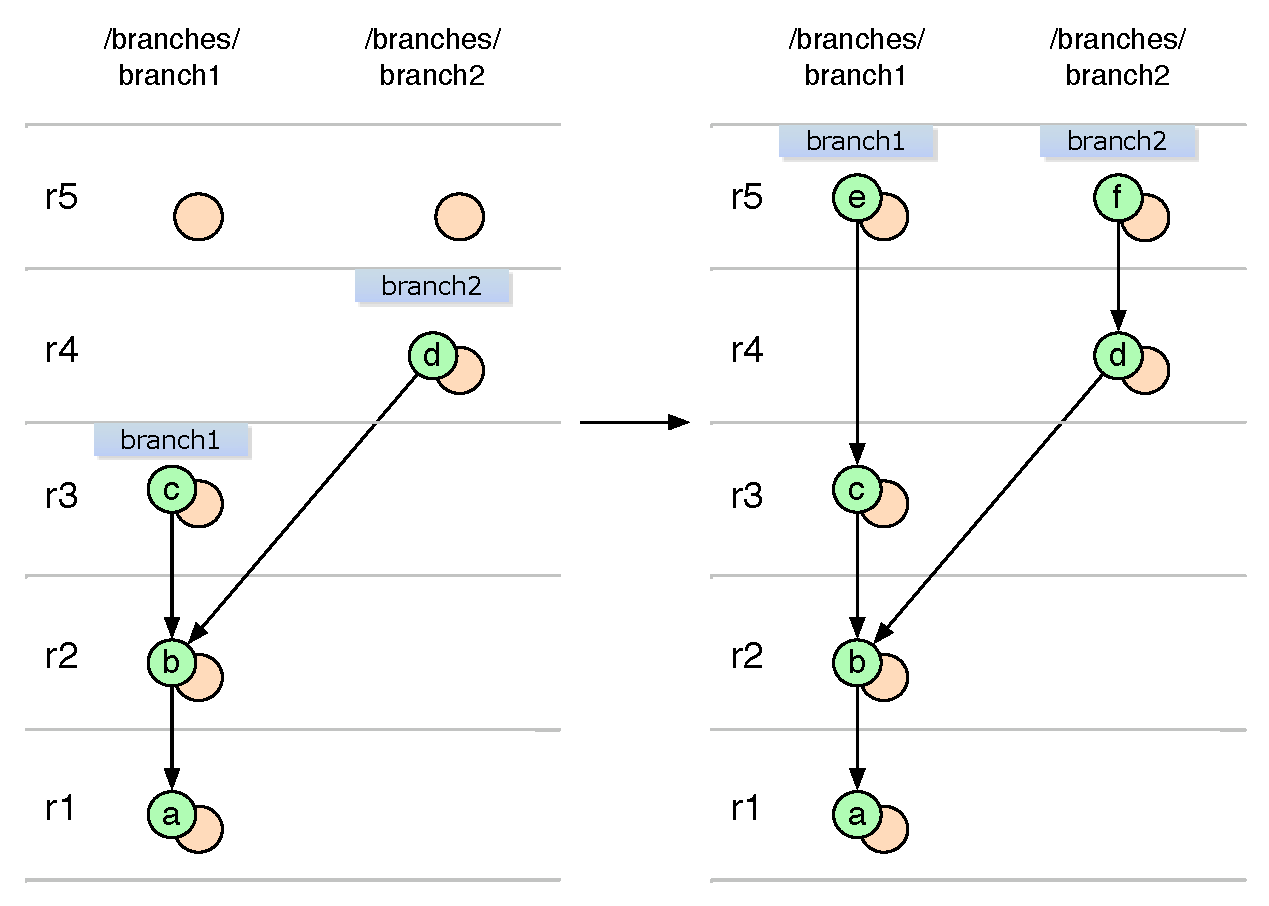
\includegraphics[width=\textwidth]{img/diagrams/double_branch_change_svn_to_git.pdf}%
\captionof{figure}{Revision modified two branches at once being translated to creation of two commits and updating corresponding branch references.}
\label{double_branch_change_svn_to_git}%
\end{center}

\subsubsection{Deletion of Subversion Branch}

Deletion of Subversion branch is always translated into deletion of the corresponding Git branch reference
as shown on the diagram \ref{branch_deletion_svn_to_git}. Single Subversion revision might delete an arbitrary number of branches, 
and thus result in multiple branch references being deleted in Git repository on translation.
\begin{center}
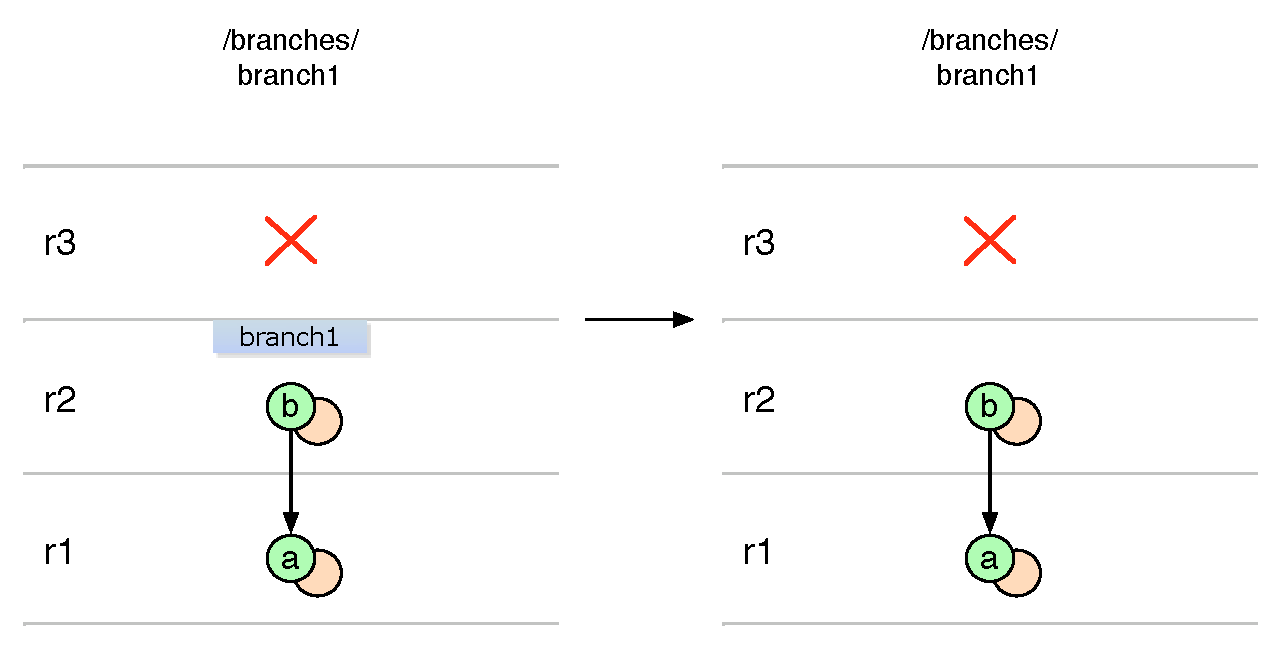
\includegraphics[width=\textwidth]{img/diagrams/branch_deletion_svn_to_git.pdf}%
\captionof{figure}{Deletion of Subversion branch being translated to Git branch removal.}
\label{branch_deletion_svn_to_git}%
\end{center}

\subsubsection{Replacement of Subversion Branch}

Subversion user is able to replace one branch by another with the same name.
Translation of that special case is performed as shown on diagram \ref{branch_replacement_svn_to_git}.
\begin{center}
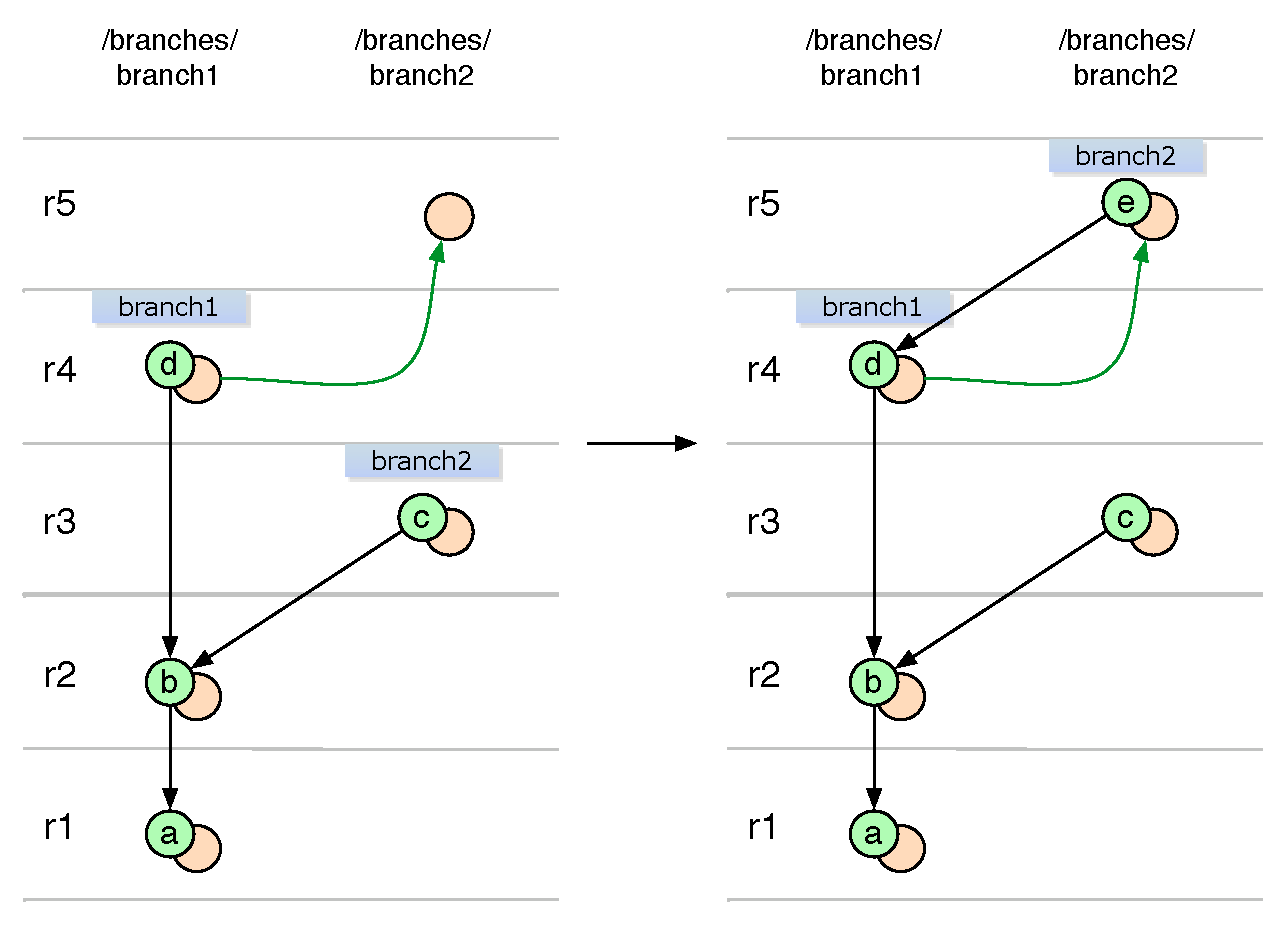
\includegraphics[width=\textwidth]{img/diagrams/branch_replacement_svn_to_git.pdf}%
\captionof{figure}{Replacement of Subversion branch being translated to replacement of Git branch.}
\label{branch_replacement_svn_to_git}%
\end{center}

\subsection{Git Branches and Tags}

To translate Git branches and tags into corresponding Subversion entities, Translator
constantly tracks current set of the reference objects (branches and tags) in the Git repository. Whenever 
Translator discovers that there are new, modified or deleted reference objects in the Git 
repository, it creates, modifies or deletes corresponding directory in the Subversion repository.
\subsubsection{New Git Branch}

New Git branch reference discovered might refer to the new, not yet translated Git commit object
which has parent commit (diagram \ref{branch_creation_git_to_svn}), to the new Git commit without
reference to a parent commit (diagram \ref{branch_creation_no_history_git_to_svn}) or to the 
existing Git commit (diagram \ref{svn_no_change_branch_creation_git_to_svn}).

\begin{center}
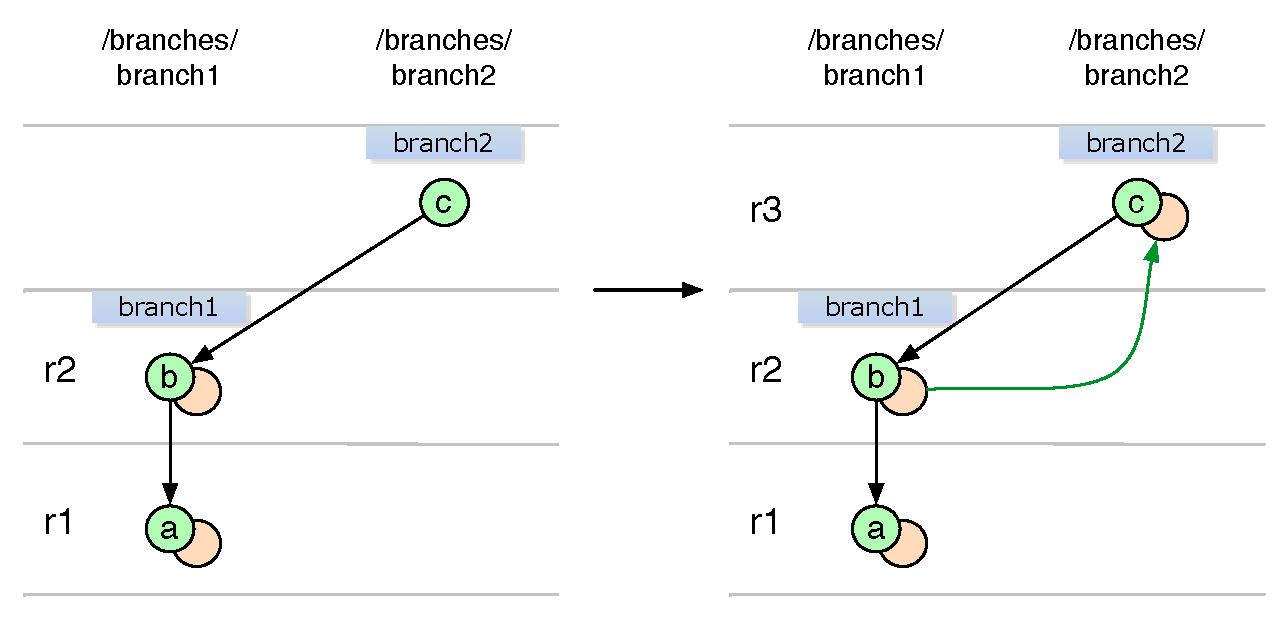
\includegraphics[width=\textwidth]{img/diagrams/branch_creation_git_to_svn.pdf}%
\captionof{figure}{Git branch addition being translated to Subversion branch copy.}
\label{branch_creation_git_to_svn}%
\end{center}

\begin{center}
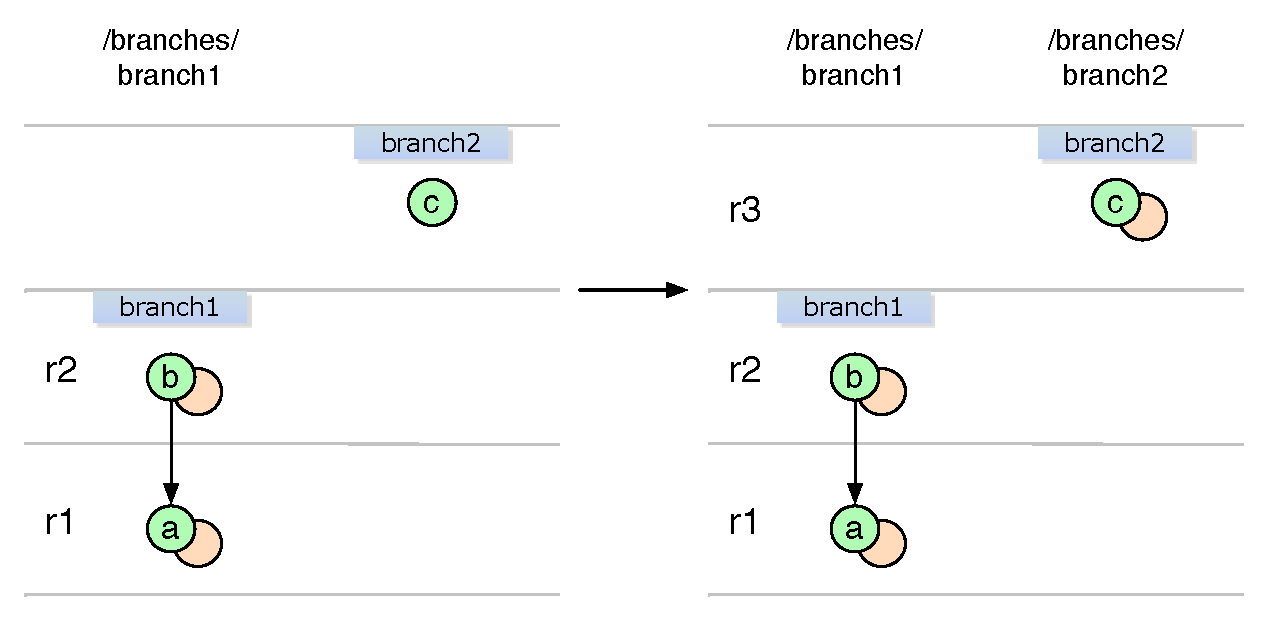
\includegraphics[width=\textwidth]{img/diagrams/branch_creation_no_history_git_to_svn.pdf}%
\captionof{figure}{Addition of Git branch referenced to commit with no parents being translated to Subversion branch creation.}
\label{branch_creation_no_history_git_to_svn}%
\end{center}

\begin{center}
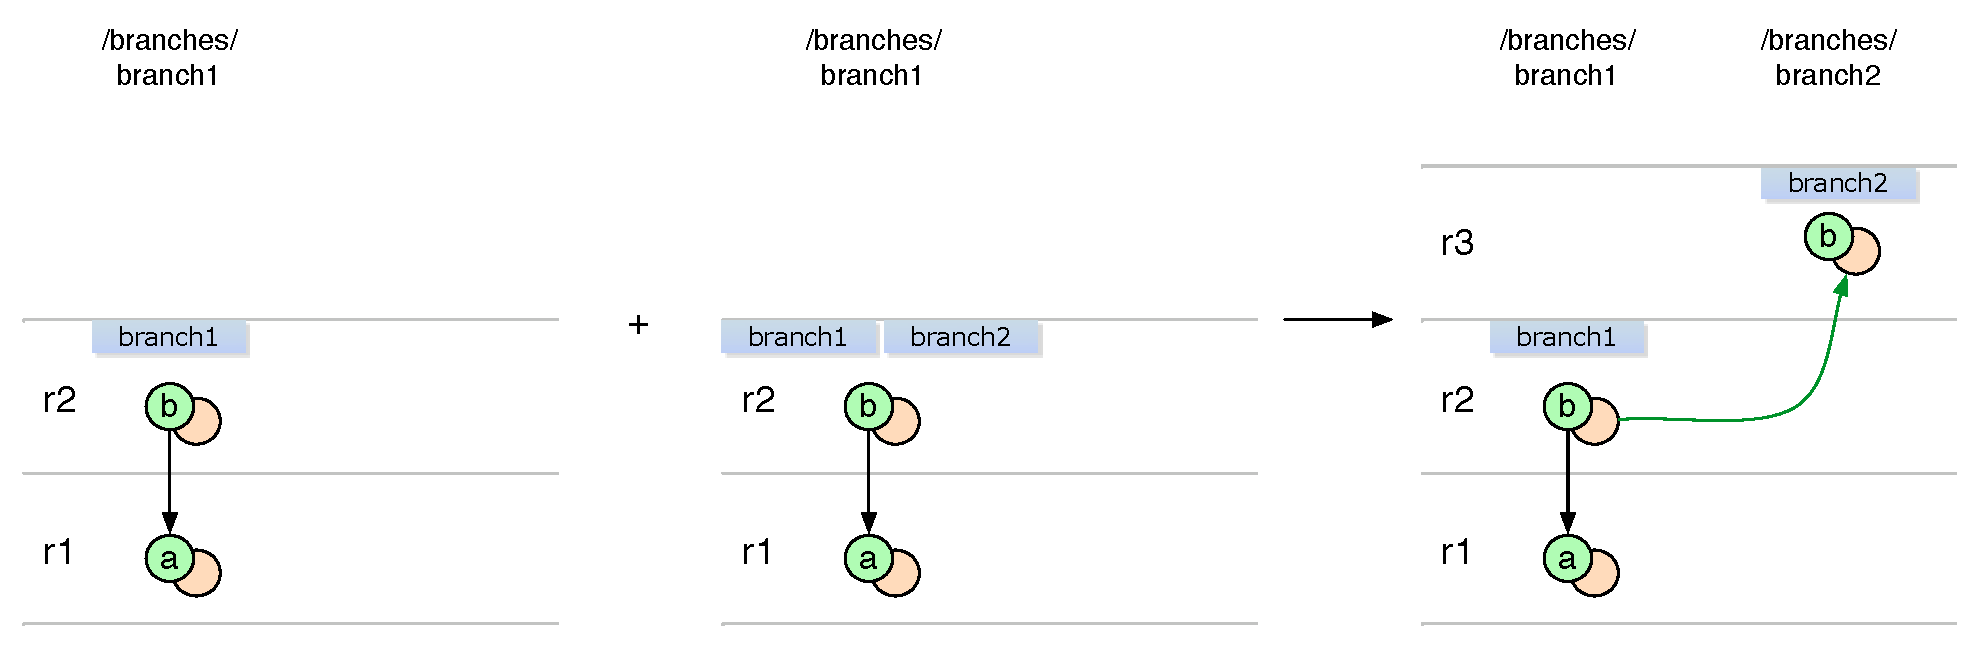
\includegraphics[width=\textwidth]{img/diagrams/svn_no_change_branch_creation_git_to_svn.pdf}%
\captionof{figure}{Addition of second reference to Git commit being translated to creation of Subversion branch with no changes.}
\label{svn_no_change_branch_creation_git_to_svn}%
\end{center}

In the last case, Subversion revision r3 is synthetic, with automatically generated commit message and commit date of the time
revision was created.
\\\\
Combination of the new Git commits on existing branch and new Git branch reference pointing to the latest commit,
is also translated into a new Subversion branch creation, as shown on the diagram \ref{ambiguous_svn_branch_git_to_svn}.
All the new Git commits are translated to the modifications of the first branch, and then as many new branches 
are copied from this first branch as there are new branch references pointing to the latest Git commit on the 
first branch.
\begin{center}
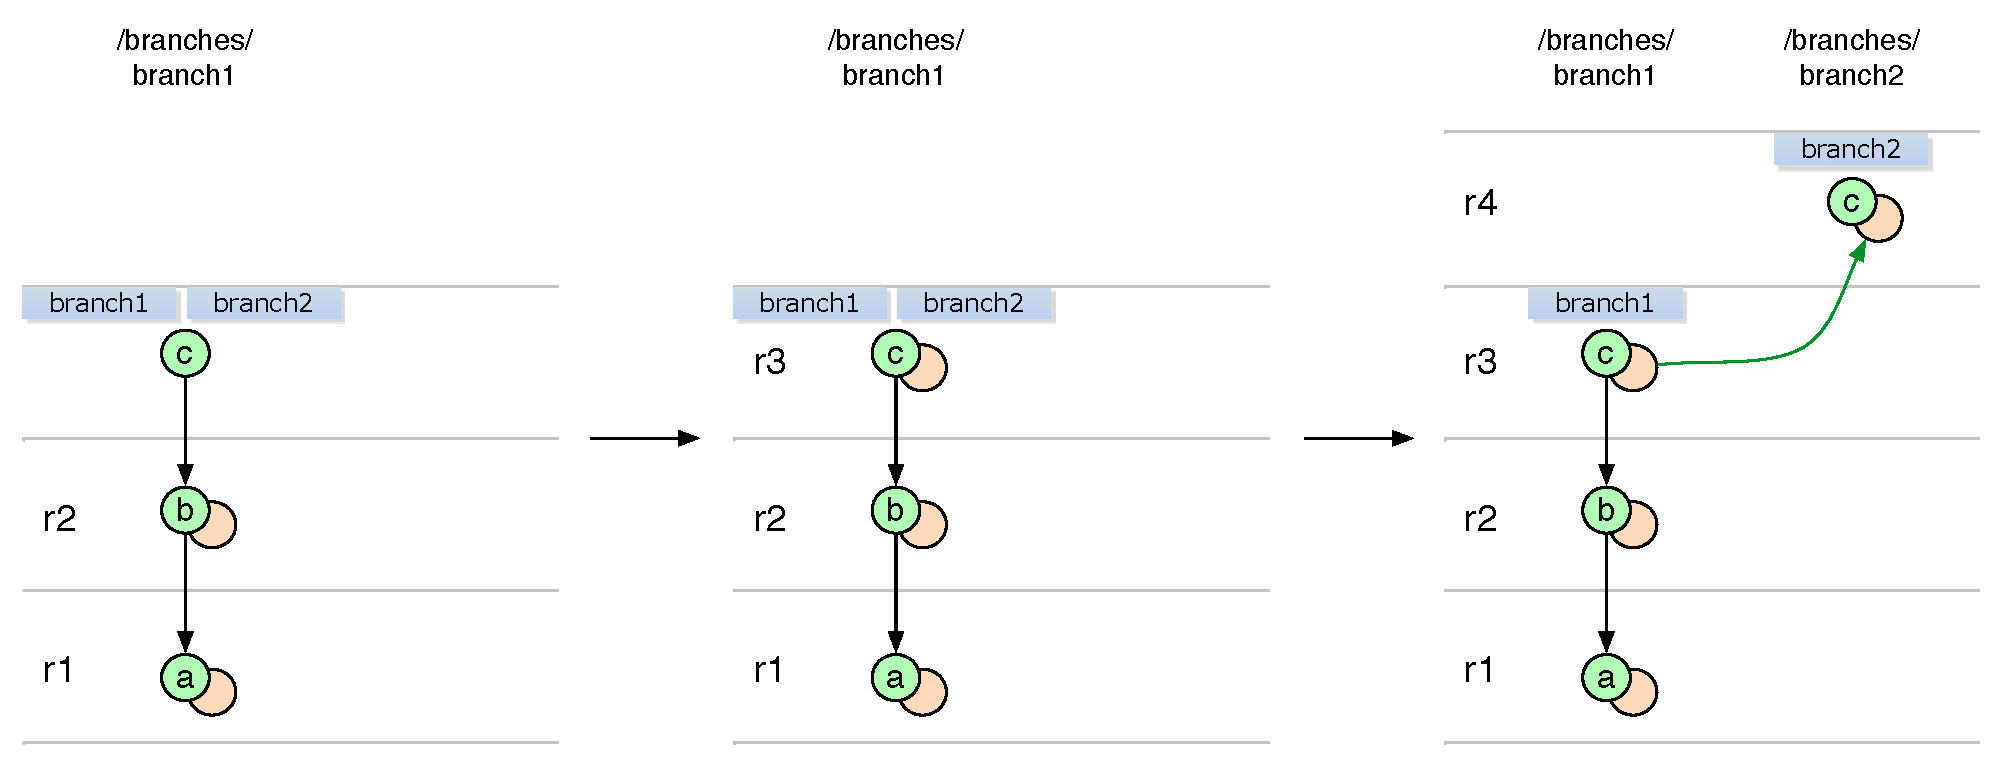
\includegraphics[width=\textwidth]{img/diagrams/ambiguous_svn_branch_git_to_svn.pdf}%
\captionof{figure}{Commit referenced by two branches being translated to Subversion two revisions: modification revision r3 and second branch creation revision r4.}
\label{ambiguous_svn_branch_git_to_svn}%
\end{center}

\subsubsection{Git Branch Deletion}

Deletion of the Git branch reference results in the deletion of the corresponding branches in Subversion repository, 
(diagram \ref{branch_deletion_git_to_svn}). Multiple Git branches could be removed at once and as a result Translator 
creates a single revision which removes every corresponding Subversion branch.
\begin{center}
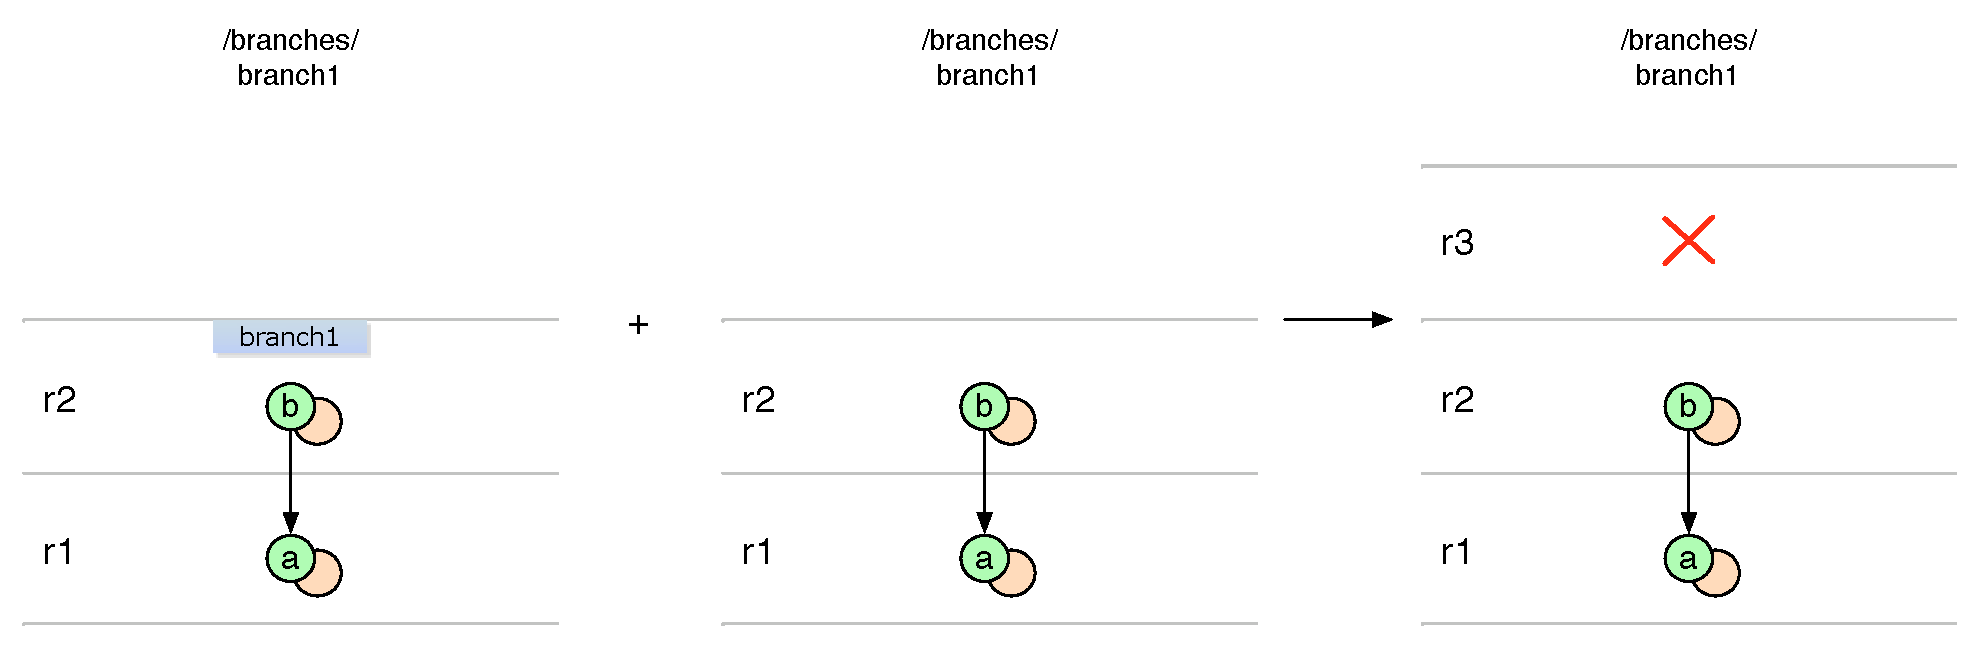
\includegraphics[width=\textwidth]{img/diagrams/branch_deletion_git_to_svn.pdf}%
\captionof{figure}{Deletion of Git branch being translated to Subversion branch removal.}
\label{branch_deletion_git_to_svn}%
\end{center}

\subsubsection{Git Branch Replacement}
Git user may reset any branch to any commit, and that kind of modification is translated as shown on the diagram \ref{branch_replacement_git_to_svn}.
\begin{center}
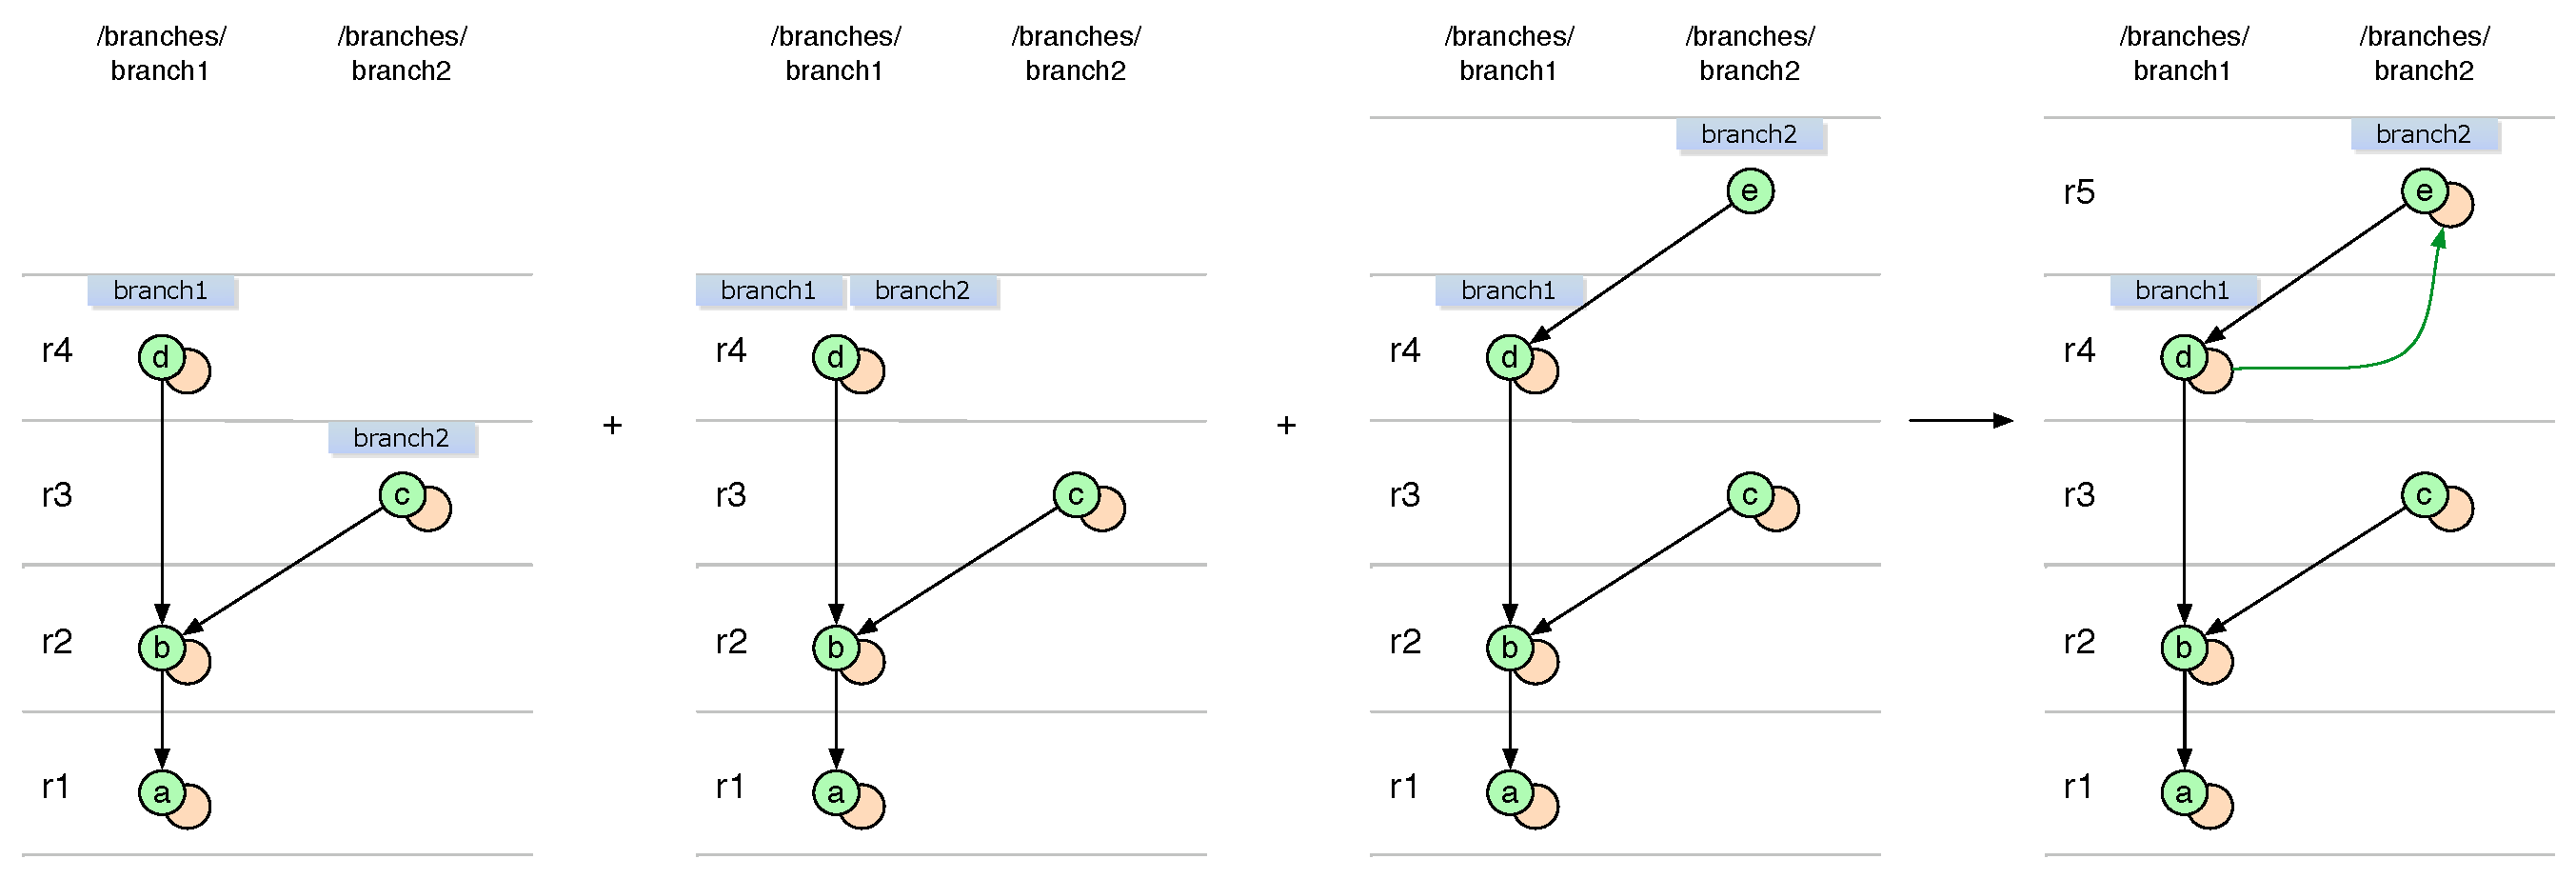
\includegraphics[width=\textwidth]{img/diagrams/branch_replacement_git_to_svn.pdf}%
\captionof{figure}{Replacement of Git branch being translated to replacement of Subversion branch.}
\label{branch_replacement_git_to_svn}%
\end{center}

\subsubsection{Unaccessible Git Commits}
Deletion or replacement of a branch might result in a Git commit becoming unaccessible and subject to the 
garbage collection. Translator should however, keep such commits around because further Subversion revisions 
may refer to these "unaccessible" commits, for instance when Subversion revision ressurrects previously
deleted branch.
\\\\
To address this problem Translator creates references to unaccessible Git commits, 
whenever such unaccessible commit is detected. 
These special references uses dedicated namespace /refs/attic and in general has a form of /refs/attic/branchName@revisionNumber.
\\\\
For instance, on diagram \ref{branch_deletion_git_to_svn} (Git branch reference is deleted), Git commit \emph{b} is referenced with /refs/attic/branch1@2 reference and on
diagram \ref{branch_replacement_git_to_svn} (Git branch reference is replaced) Git commit \emph{c} is referenced with /refs/attic/branch2@3 reference
after translation is completed.
\renewcommand{\figurename}{Diagram}
\subsection{Merge Tracking}

Both Subversion and Git tracks merges performed in repository. There are differences, however in 
the granularity of the information being kept by Git and Subversion.
\\\\
\textbf{Subversion}: information on merge sources might be set on any path (file or directory) and might include not only
merge source paths, but also particular revisions.
\\\\
\textbf{Git}: merges are represented as merge commits. Git merge commit is a Git commit which has more than a single 
ancestor. Merge commit represents changes being merged from all of the ancestor's branches into the branch (or branches)
merge commit belongs to.
\\\\
\textbf{Translator}: merges are interpreted in terms of the source branches being merged into a 
target branch in particular commit or revision. This sort of interim interpretation allows Translator
to represent any merge commit in Git repository, as well as most common merge scenarios in Subversion repositories (merges
between branches).
\\\\
There are no means to represent some of the Subversion merge scenarios in terms of that interim language.
Such merges, which includes cherry-pick merges, merges on files or on non-branch directories are ignored by the Translator,
i.e. are translated to a regular Git commits with a single ancestor.

\subsubsection{Translation of the Git Merge Commit}

Git merge commit (commit with multiple ancestors) is translated into Subversion revision in two steps.
\begin{itemize}
\item Git commit is translated into Subversion revision, accordingly to the rules described in "Revisions and Commits" section.
This new revision, by definition, only affects single Subversion branch directory.
\item \textbf{svn:mergeinfo} property is updated on the affected Subversion branch directory so, that all merge
commit ancestor branches are considered to be merged into this very branch in this very revision.
\end{itemize}

Example of such translation is shown in the diagram \ref{simple_merge_git_to_svn}:

\begin{center}
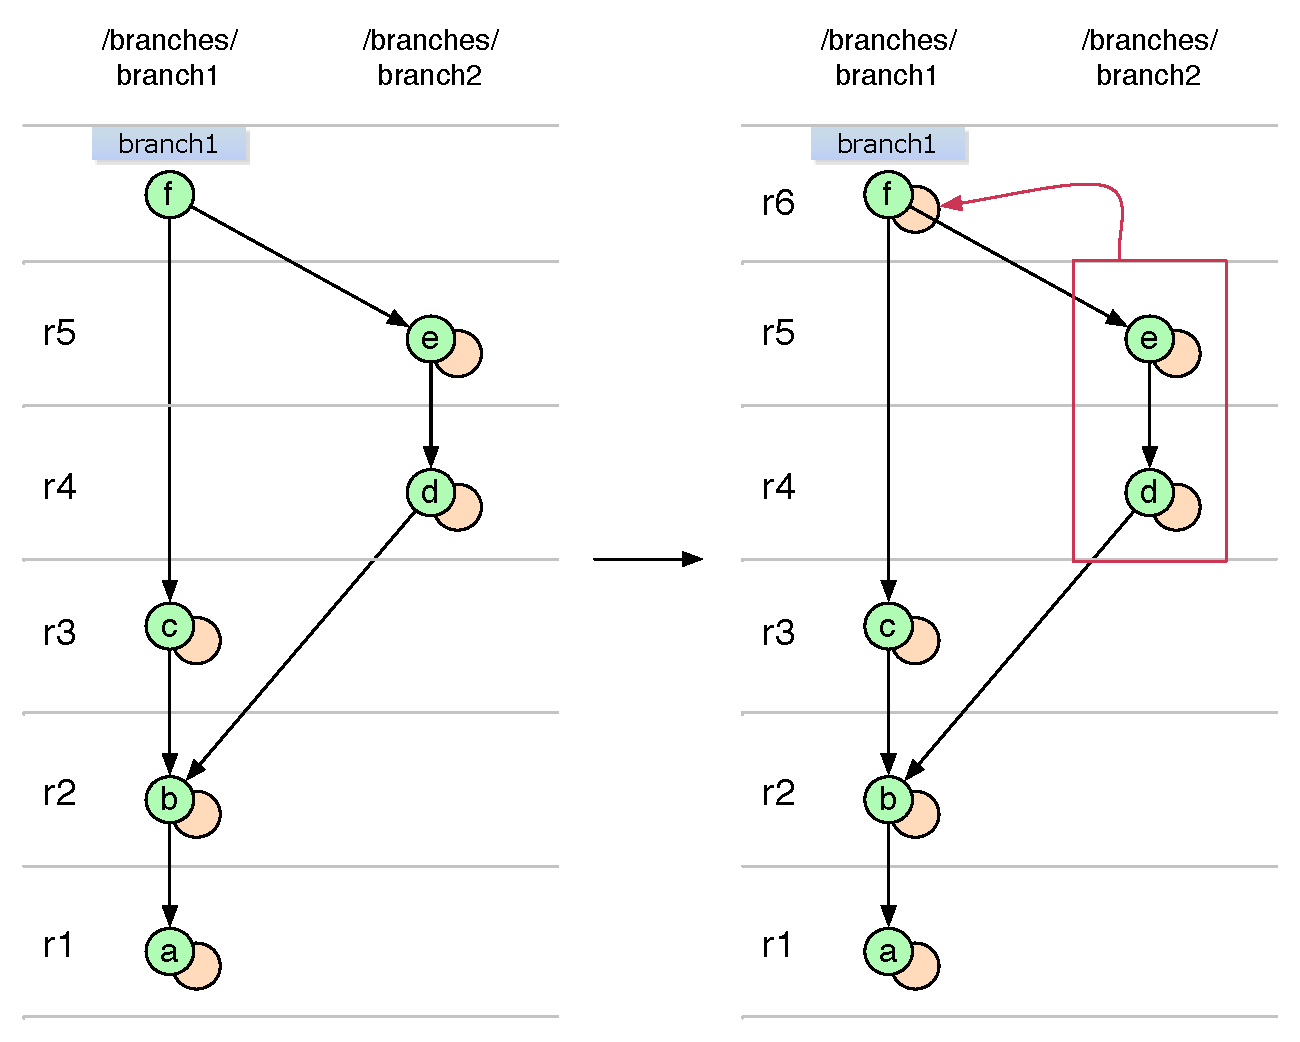
\includegraphics[width=\textwidth]{img/diagrams/simple_merge_git_to_svn.pdf}%
\captionof{figure}{Git merge commit being translated to the change of svn:mergeinfo property.}
\label{simple_merge_git_to_svn}%
\end{center}

Revision \emph{6} is created as a result of commit \emph{f} translation. Then svn:mergeinfo property is updated on /branches/branch1 directory
(red arrow) to reflect merge of commits \emph{d} and \emph{e} made on /branches/branch2 into /branches/branch1. In this 
particular example svn:mergeinfo on /branhces/branch1 will be set to "/branches/branch2:4-5" value.
\\\\
Only commits made on the source (ancestor) branches are included into Subversion svn:mergeinfo, references to the commits on the same branch
are excluded. For instance, in the example above, svn:mergeinfo will not contain "/branches/branch1:1-2". Thus, translation of the merge commit with no common history will result in the same svn:mergeinfo being set in Subversion repository (see diagram \ref{simple_merge_branch_no_parent_git_to_svn})

\begin{center}
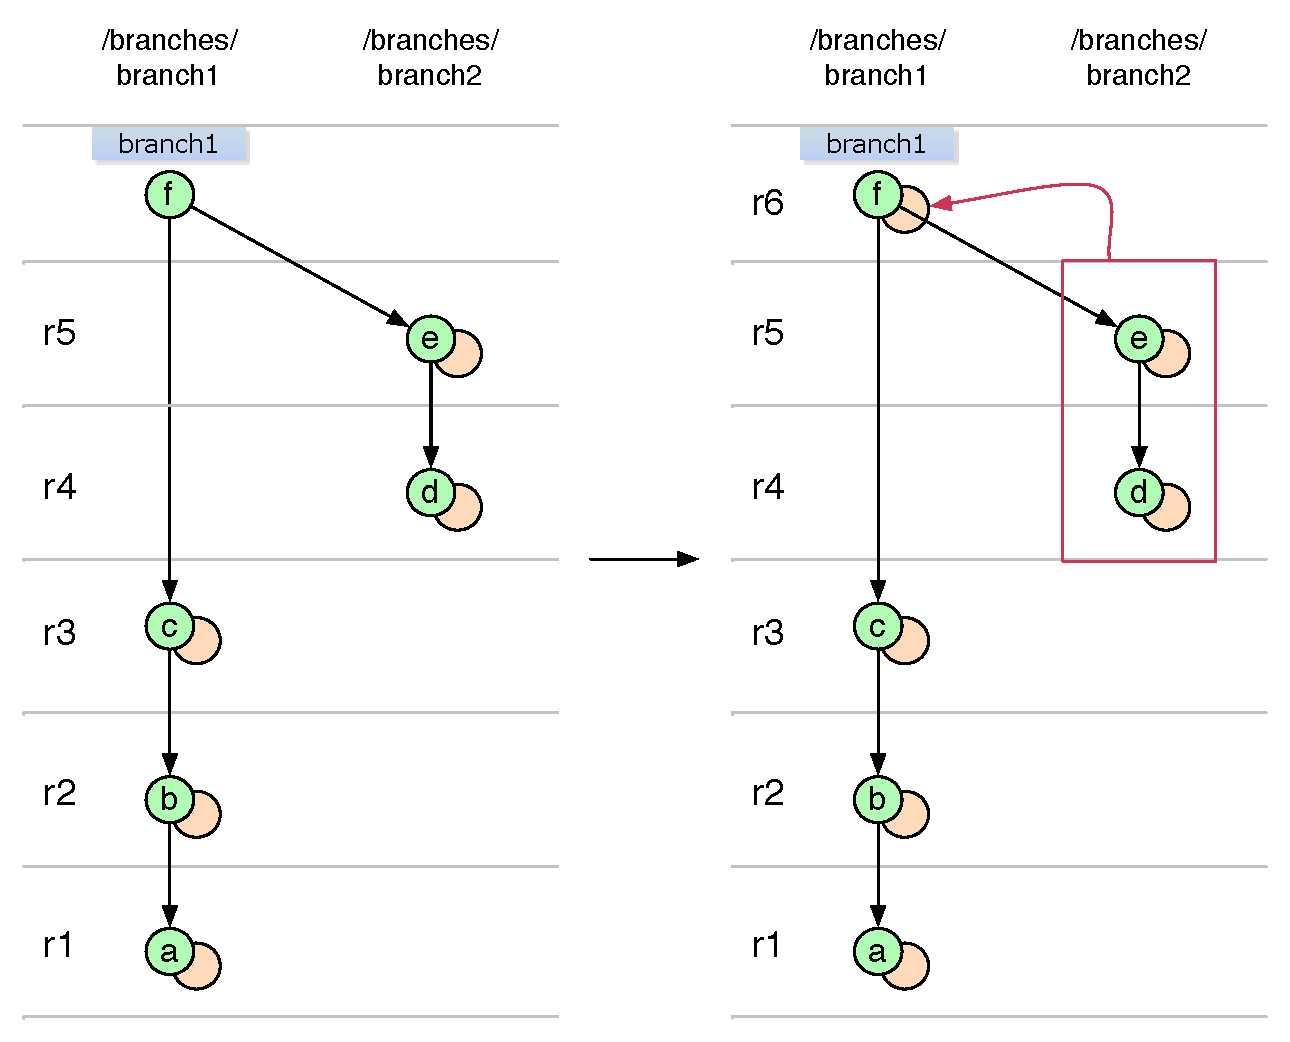
\includegraphics[width=\textwidth]{img/diagrams/simple_merge_branch_no_parent_git_to_svn.pdf}%
\captionof{figure}{Git merge commit being translated to the change of svn:mergeinfo property.}
\label{simple_merge_branch_no_parent_git_to_svn}%
\end{center}

\subsubsection{Translation of Subverion Merges}

Merge in Subversion is represented as a change of svn:mergeinfo property.
\\\\
Whenever such change of snv:mergeinfo is made on a branch directory and in 
such a way that svn:mergeinfo includes continuous ranges of revisions
made on one ore more branches (each range starting from the first revision of the branch), then that svn:mergeinfo modification is translated into a Git merge commit.
\\\\
Just like with translation of the Git merge commit into Subversion revision, 
translation in the opposite direction is performed in two steps:
\begin{itemize}
\item Git commit corresponding to the Subversion revision being translated is created accordingly 
to the rules described in "Revisions and Commits" section.
\item Additional parent commits are set on the created Git commit - one parent for each branch
referenced by Subversion svn:mergeinfo property.
\end{itemize}
Diagrams \ref{simple_merge_svn_to_git} and \ref{simple_merge_branch_no_parent_svn_to_git} provides
examples of svn:mergeinfo property (shown as a red arrow) change translation into Git Merge commit (commit \emph{f} on both
diagrams).

\begin{center}
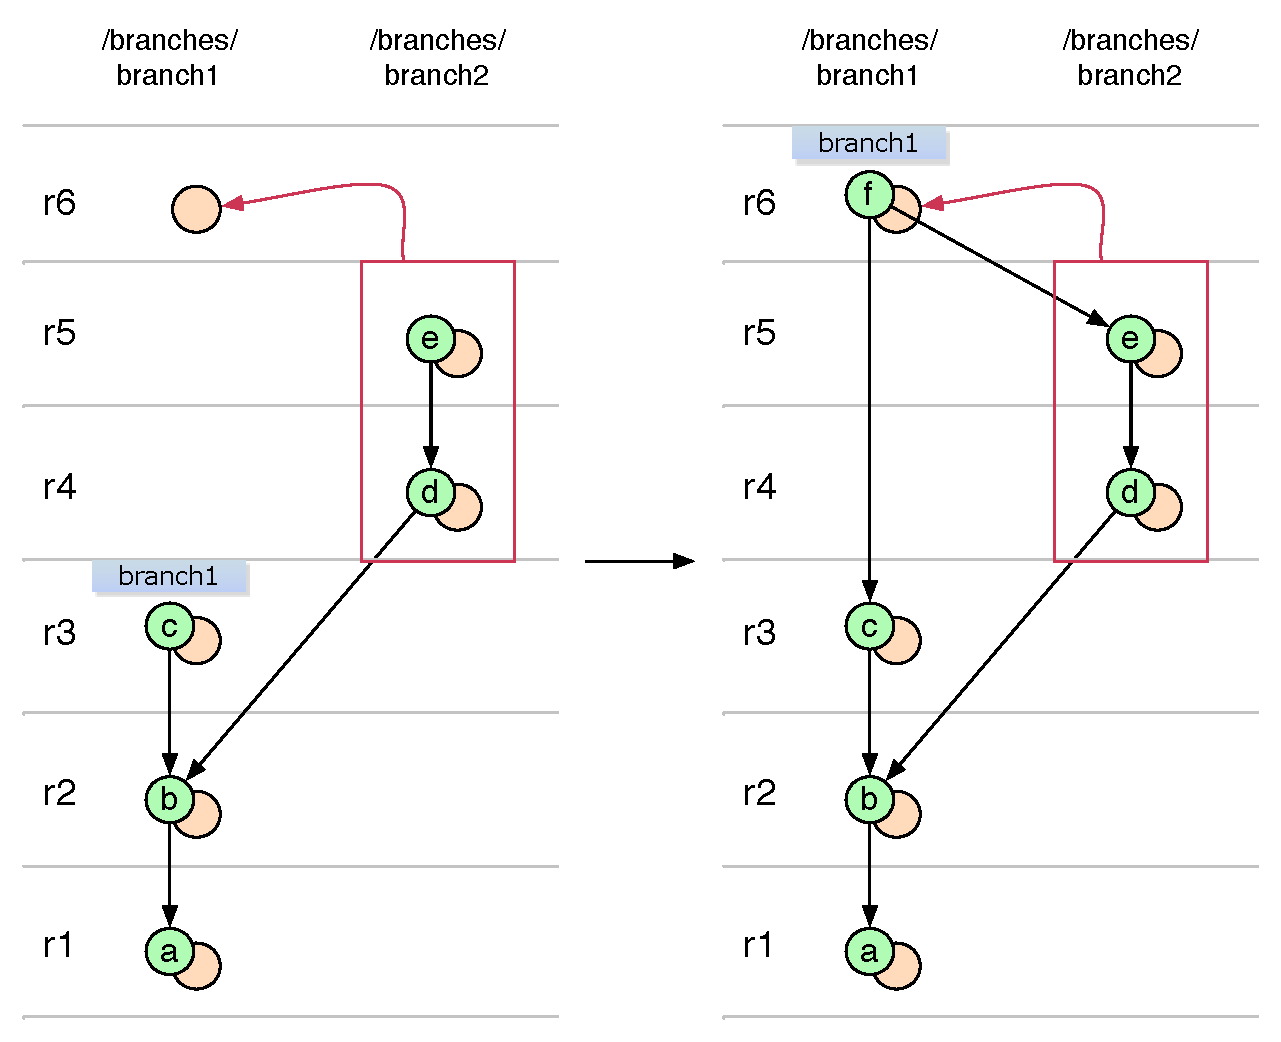
\includegraphics[width=\textwidth]{img/diagrams/simple_merge_svn_to_git.pdf}%
\captionof{figure}{svn:mergeinfo property change being translated into merge commit creation.}
\label{simple_merge_svn_to_git}%
\end{center}

\begin{center}
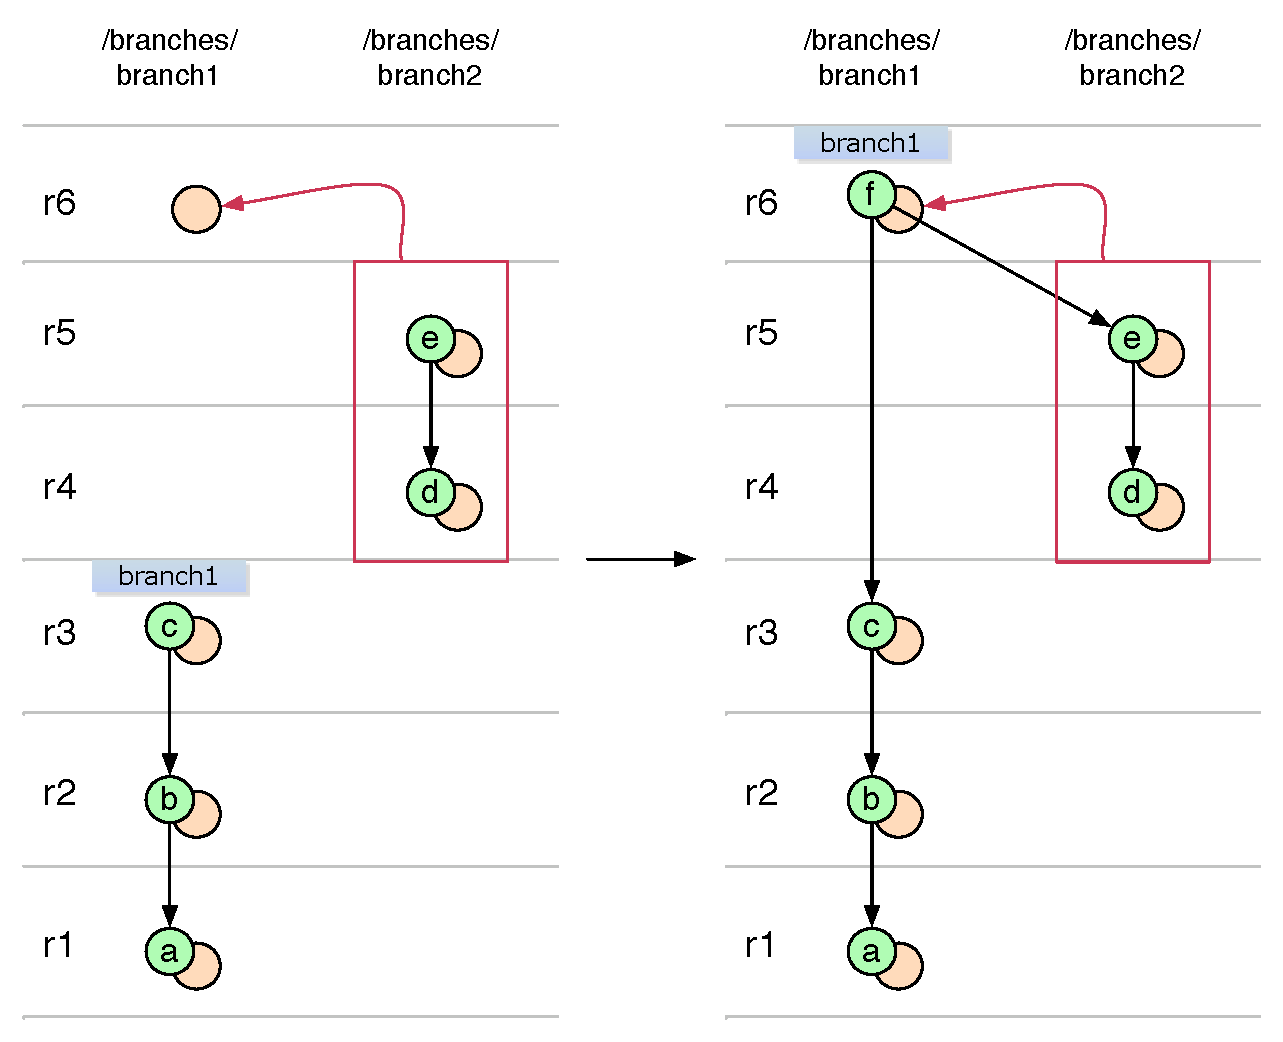
\includegraphics[width=\textwidth]{img/diagrams/simple_merge_branch_no_parent_svn_to_git.pdf}%
\captionof{figure}{svn:mergeinfo property change being translated into merge commit creation.}
\label{simple_merge_branch_no_parent_svn_to_git}%
\end{center}

\subsubsection{Subversion Cherry-Pick Merges}

Subversion tracks merges of the individual revisions, feature also known as cherry-pick merges. 
Git has no means to express merge of the individual commits, hence changes of the svn:mergeinfo Subversion
property that result from the cherry-pick merge (i.e. changes that add individual revisions to the svn:mergeinfo) are
translated into the regular Git commit with a single parent commit (see diagram \ref{no_merge_commit_on_cherry_pick_svn_to_git}).
\begin{center}
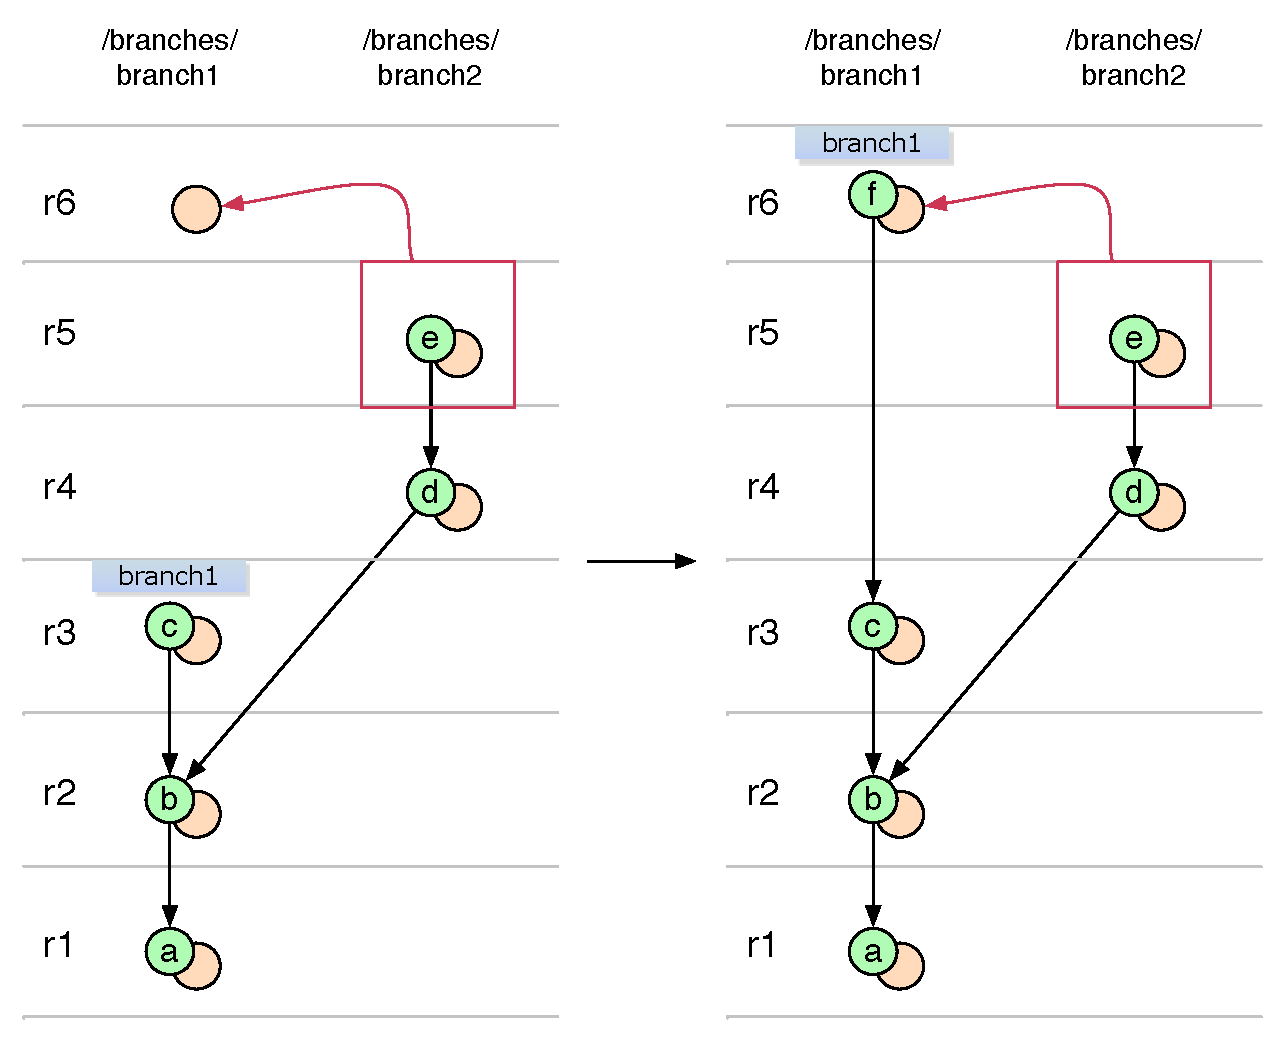
\includegraphics[width=\textwidth]{img/diagrams/no_merge_commit_on_cherry_pick_svn_to_git.pdf}%
\captionof{figure}{Cherry-pick merge being translated to ordinary commit.}
\label{no_merge_commit_on_cherry_pick_svn_to_git}%
\end{center}

Eventually, a sequence of cherry-pick merges may result in svn:mergeinfo property referring to the 
continuous range of revisions on the merge source branch, starting from the first revision 
of that branch. This last modification of svn:mergeinfo is translated into Git merge commit, as 
shown on the diagrams \ref{merge_commit_on_double_cherry_pick_svn_to_git} and \ref{merge_commit_on_double_cherry_pick_branch_no_parent_svn_to_git}.

\begin{center}
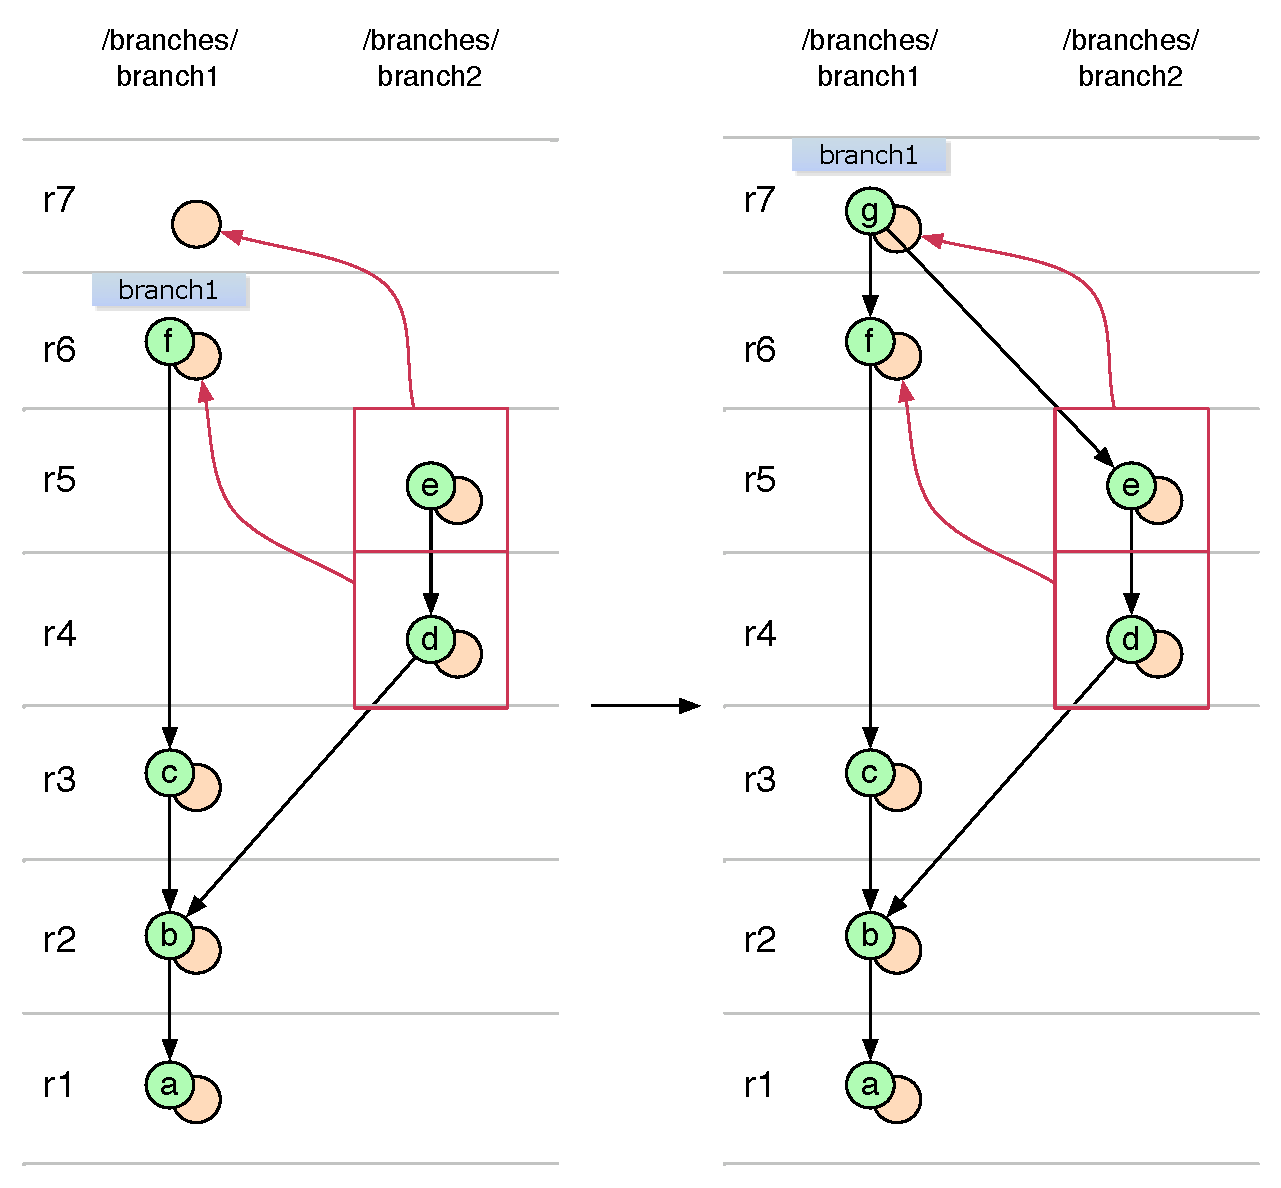
\includegraphics[width=\textwidth]{img/diagrams/merge_commit_on_double_cherry_pick_svn_to_git.pdf}%
\captionof{figure}{A sequence of cherry-pick merges being translated to merge commit.}
\label{merge_commit_on_double_cherry_pick_svn_to_git}%
\end{center}

\begin{center}
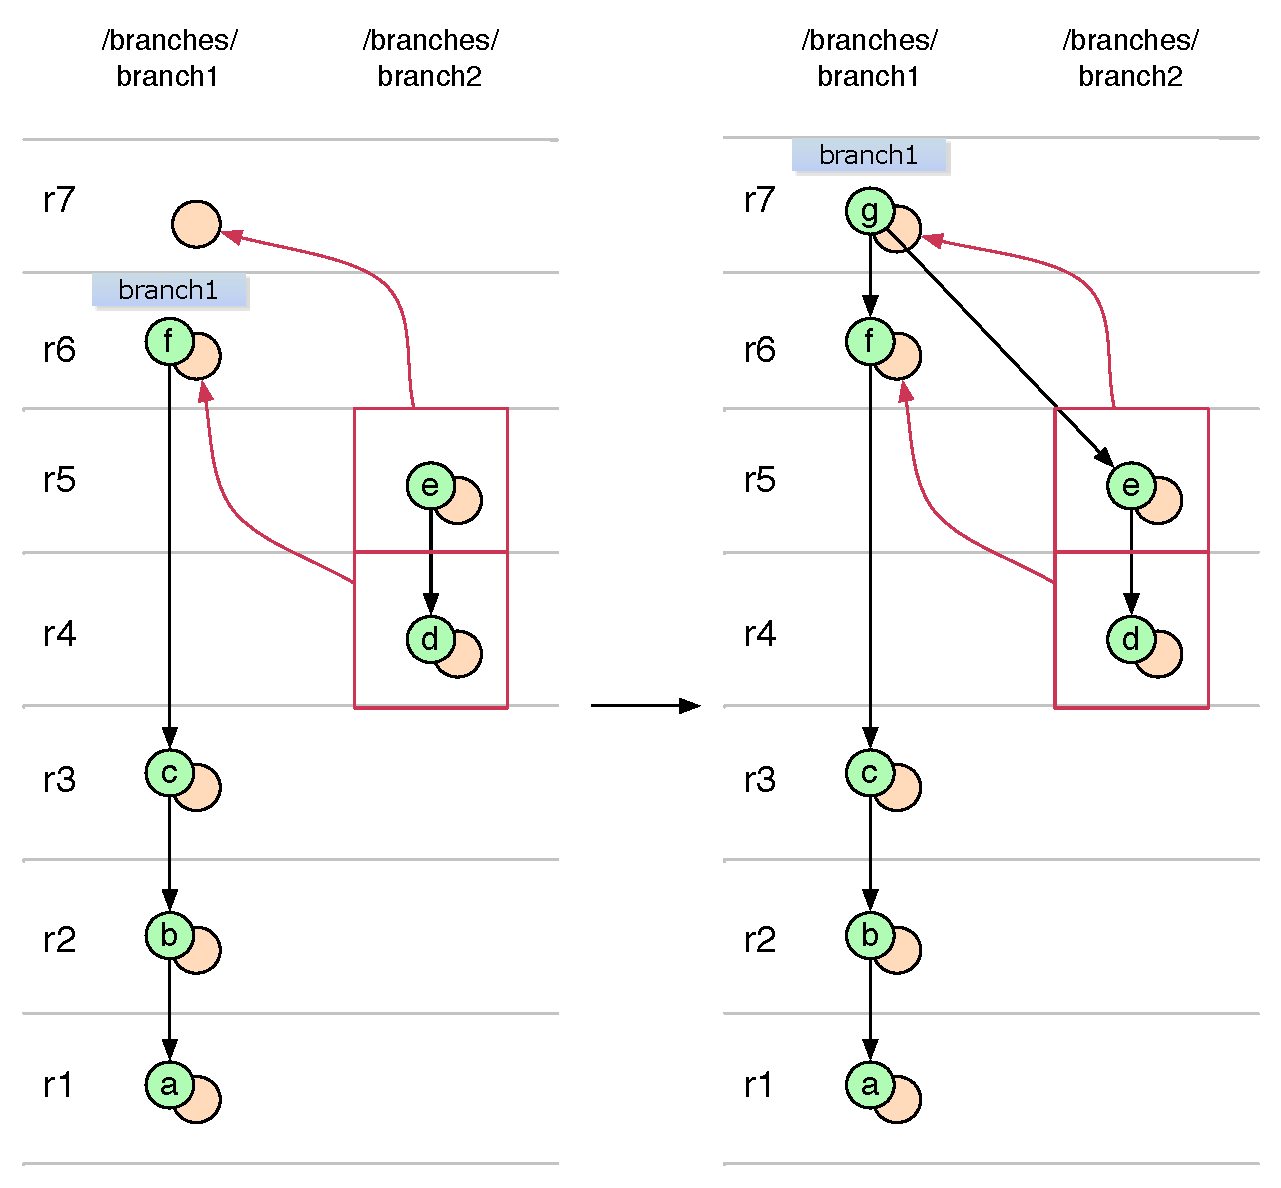
\includegraphics[width=\textwidth]{img/diagrams/merge_commit_on_double_cherry_pick_branch_no_parent_svn_to_git.pdf}%
\captionof{figure}{A sequence of cherry-pick merges being translated to merge commit.}
\label{merge_commit_on_double_cherry_pick_branch_no_parent_svn_to_git}%
\end{center}

\subsubsection{Shelf Branches}

Git user is able to push an arbitrary number of commits at once. This set of Git commits might include Git merge commit, 
so that some of the Git commits in the set are arranged into the structure we call \emph{shelf}. In general, \emph{shelf}
translation includes:
\begin{itemize}
\item Creation of a temporary Subversion branch which correspond to the \emph{shelf};
\item Translation of the "shelved" commits into revisions on that temporary branch;
\item Translation of the merge commit into revision on the main branch, with svn:mergeinfo including all revisions
of the temporary branch.
\end{itemize}
Examples of \emph{shelf} translation are shown in the diagrams \ref{boat_merge_named_shelve_git_to_svn} and \ref{boat_merge_shelve_is_normal_branch_git_to_svn}.
In these examples it is possible to determine name of the temporary branch either because branch reference points directly to the 
last \emph{shelf} commit (diagram \ref{boat_merge_named_shelve_git_to_svn}) or to the commit originating from the \emph{shelf} (diagram \ref{boat_merge_shelve_is_normal_branch_git_to_svn}).
\begin{center}
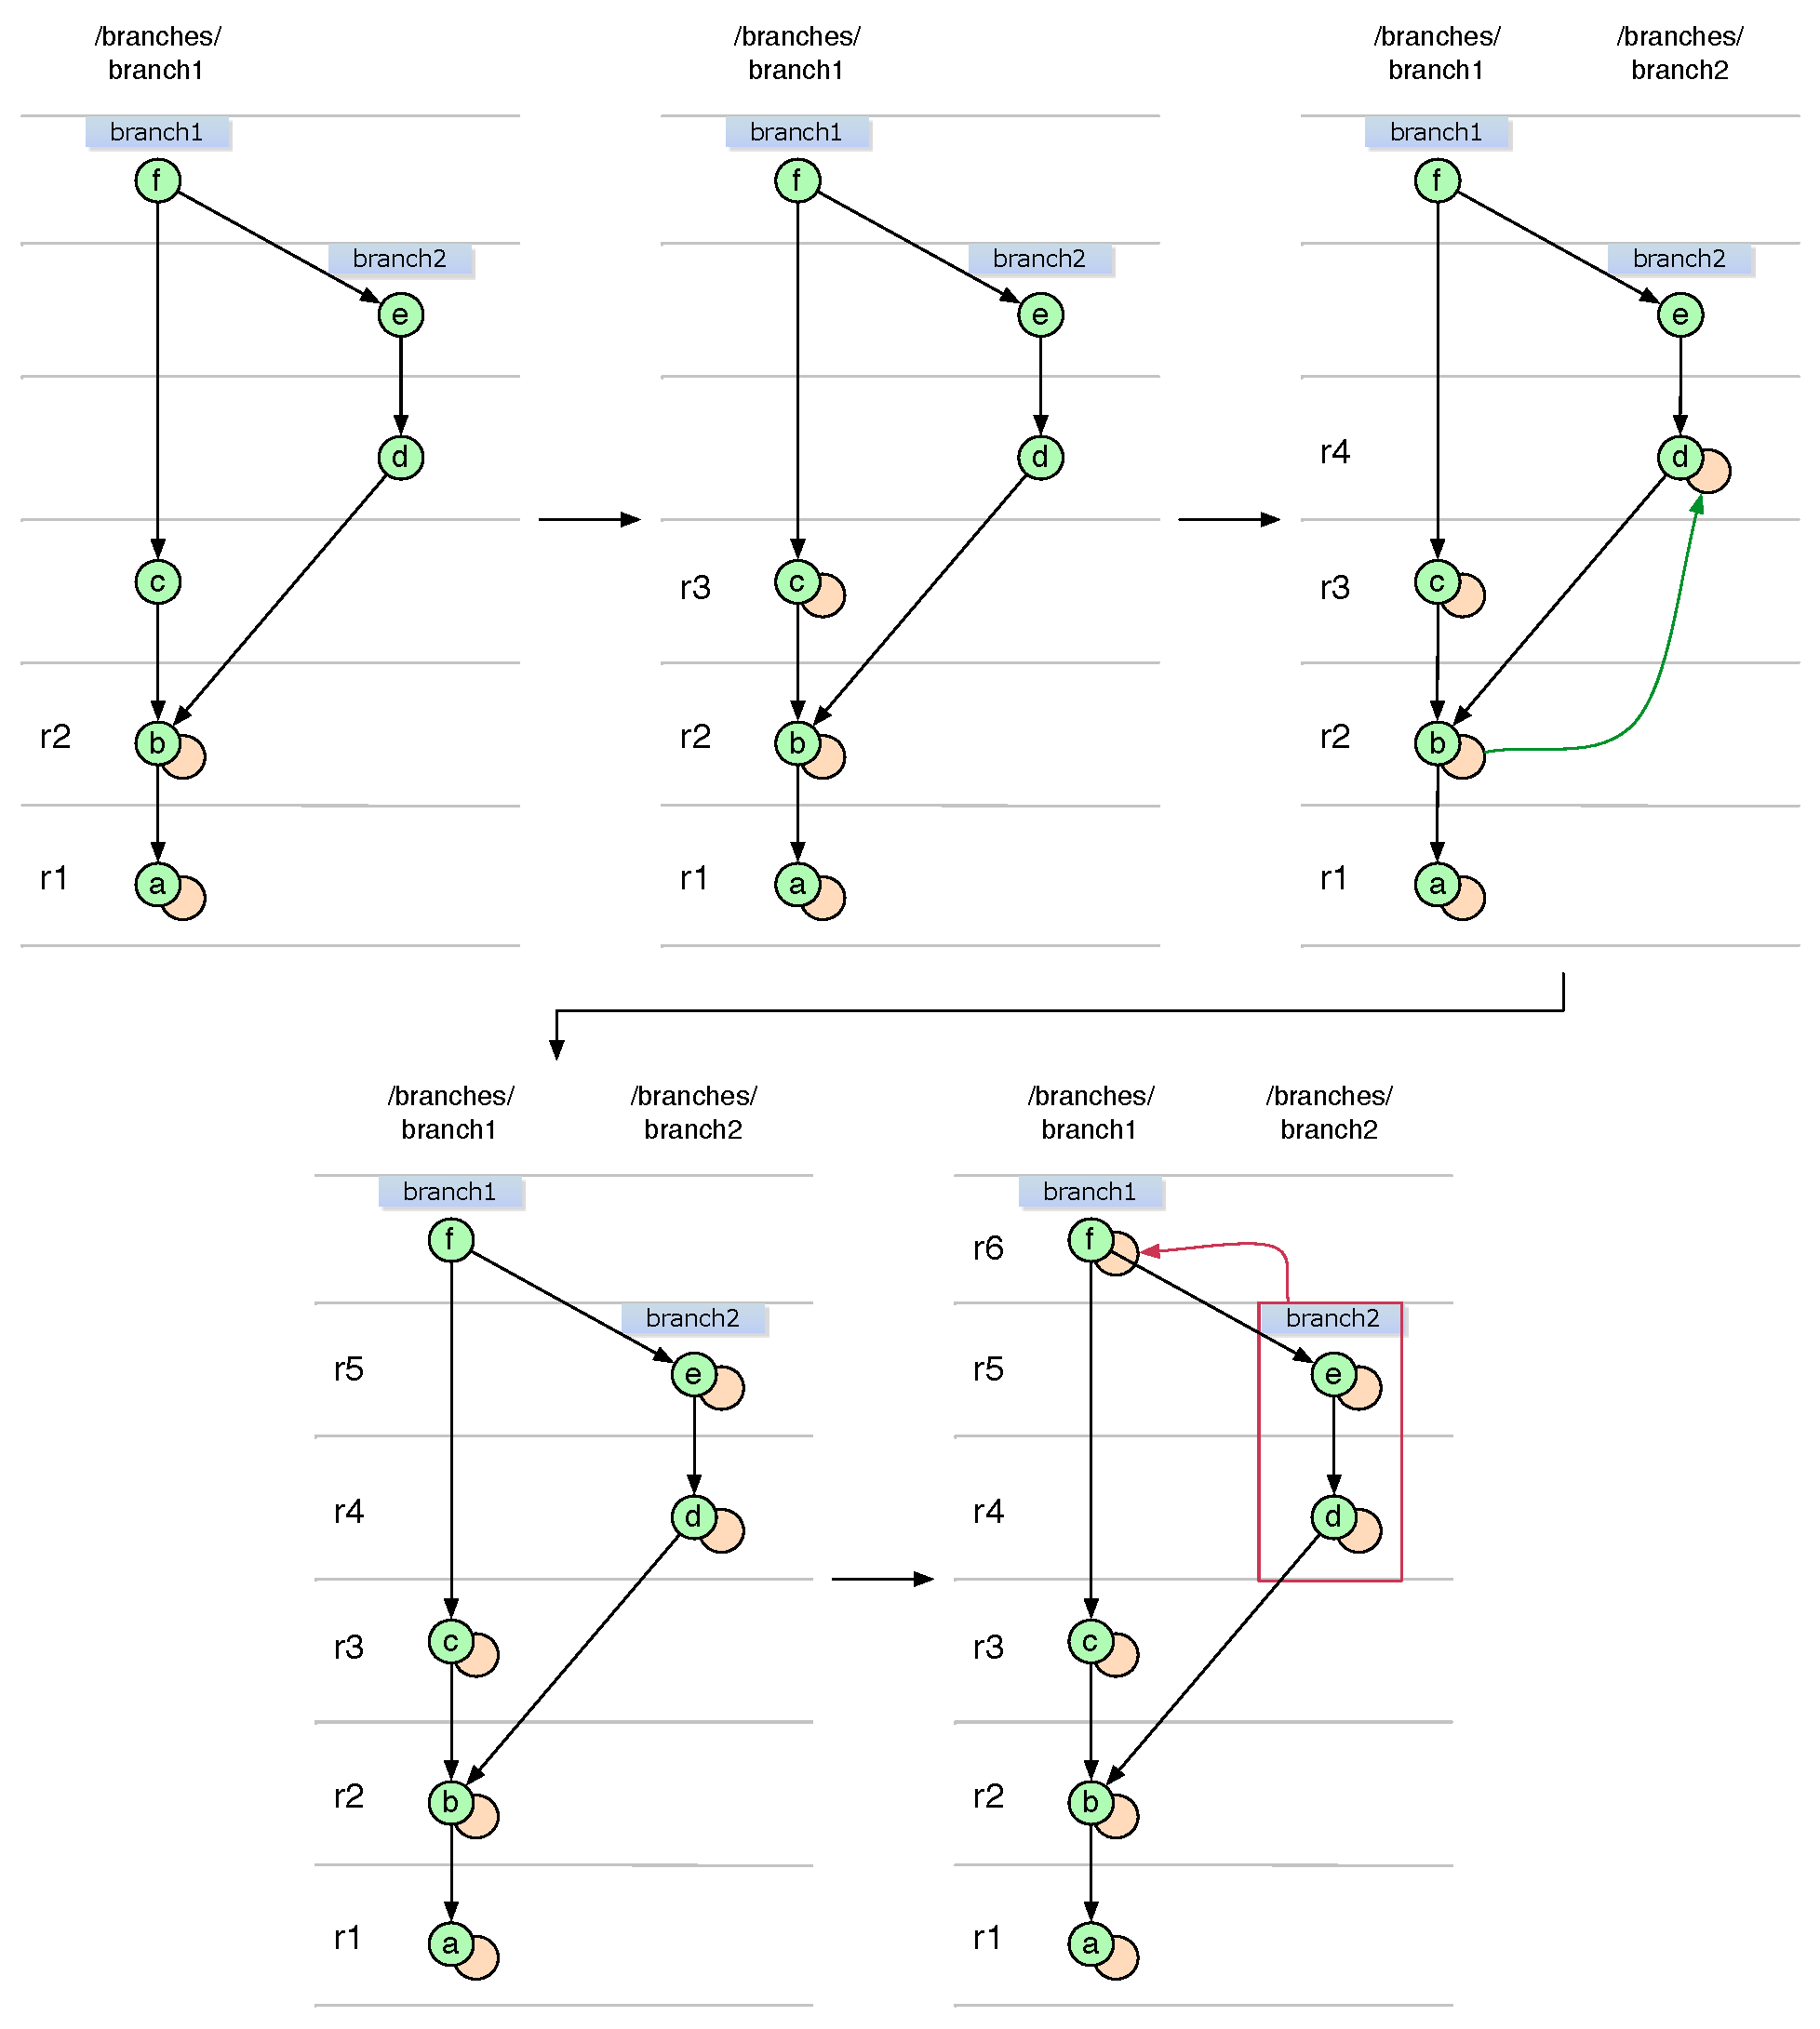
\includegraphics[width=\textwidth]{img/diagrams/boat_merge_named_shelve_git_to_svn.pdf}%
\captionof{figure}{Merge of Git branch which is available from another branch being translated to a sequence of Subversion revisions.}
\label{boat_merge_named_shelve_git_to_svn}%
\end{center}
\begin{center}
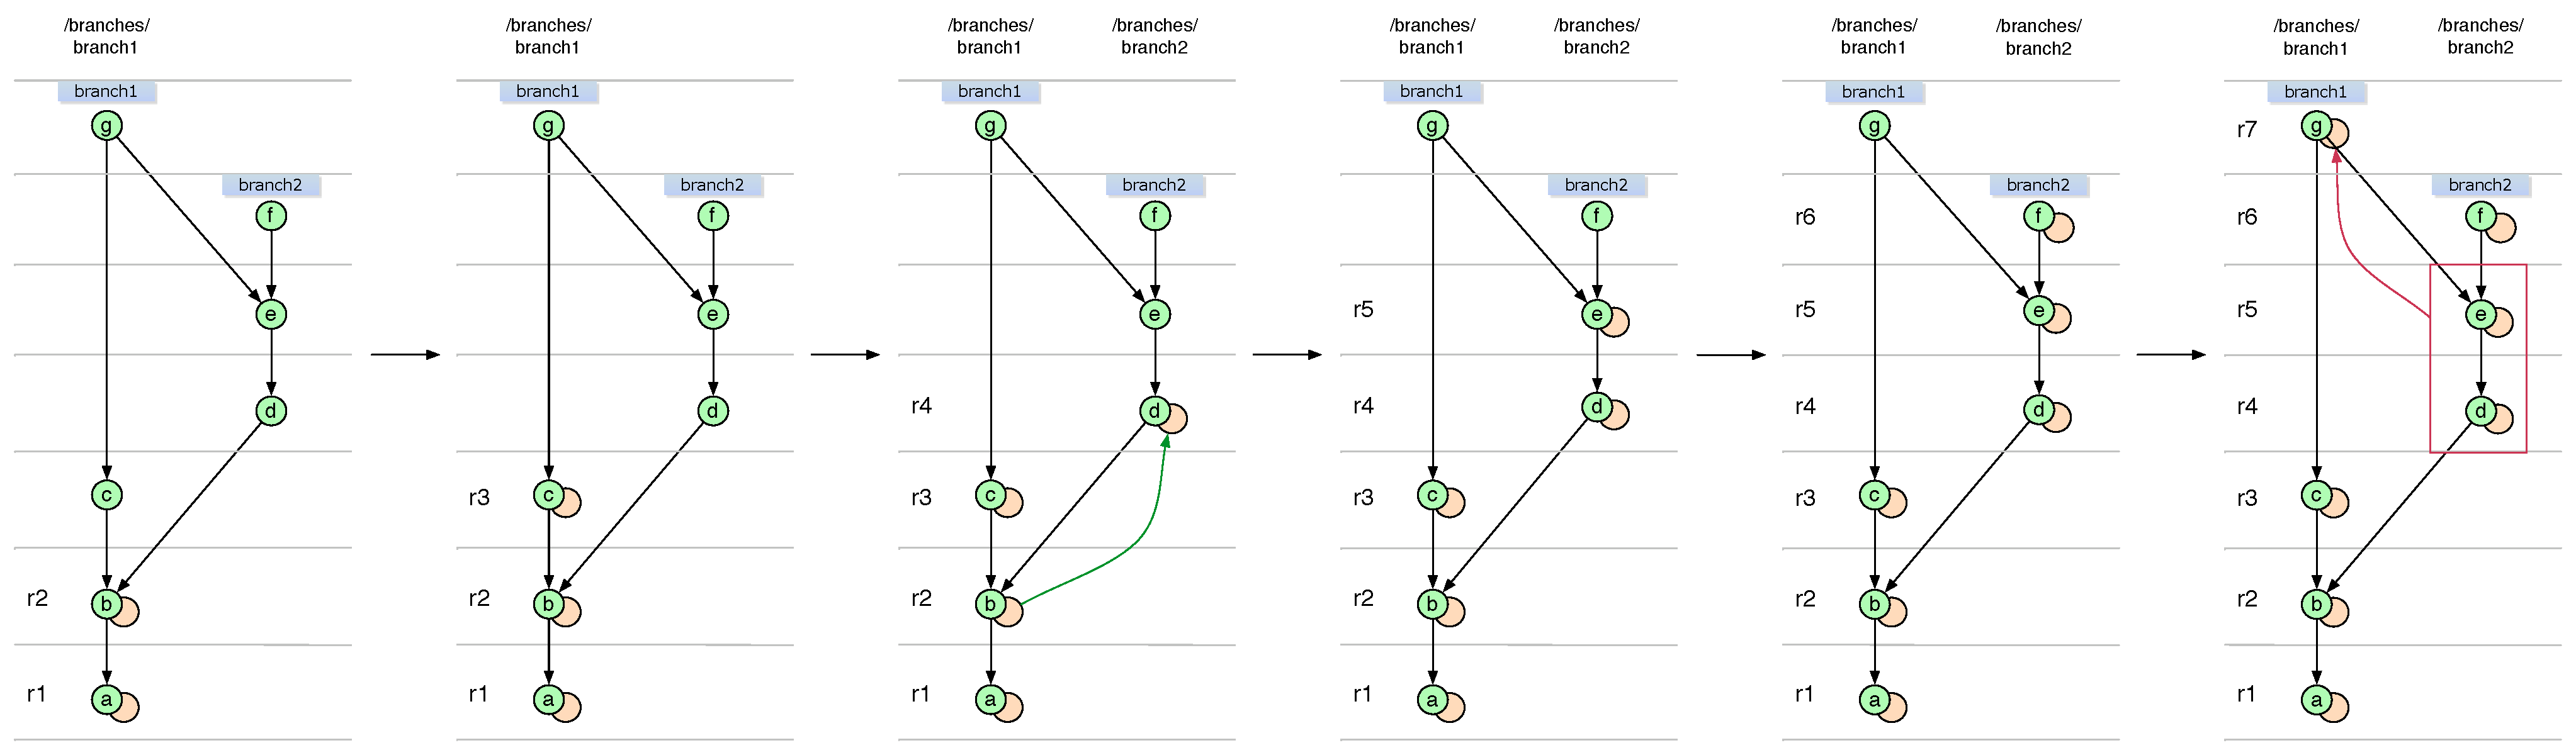
\includegraphics[width=\textwidth]{img/diagrams/boat_merge_shelve_is_normal_branch_git_to_svn.pdf}%
\captionof{figure}{Merge of Git branch which is available from another branch being translated to a sequence of Subversion revisions.}
\label{boat_merge_shelve_is_normal_branch_git_to_svn}%
\end{center}

In certain cases, it is not possible to determine name of the temporary branch, as there is no branch reference pointing to
the \emph{shelved} commits. In such case Translator creates temporary branch named after last shelf commit author and 
deletes this temporary branch in the revision which corresponds to the merge commit (see diagram \ref{boat_merge_git_to_svn}). 
\\\\
To reduce clutter, anonymous temporary branch is created in the /shelves/ top-level Subversion directory, not in the /branches/ one where named branches reside.

\begin{center}
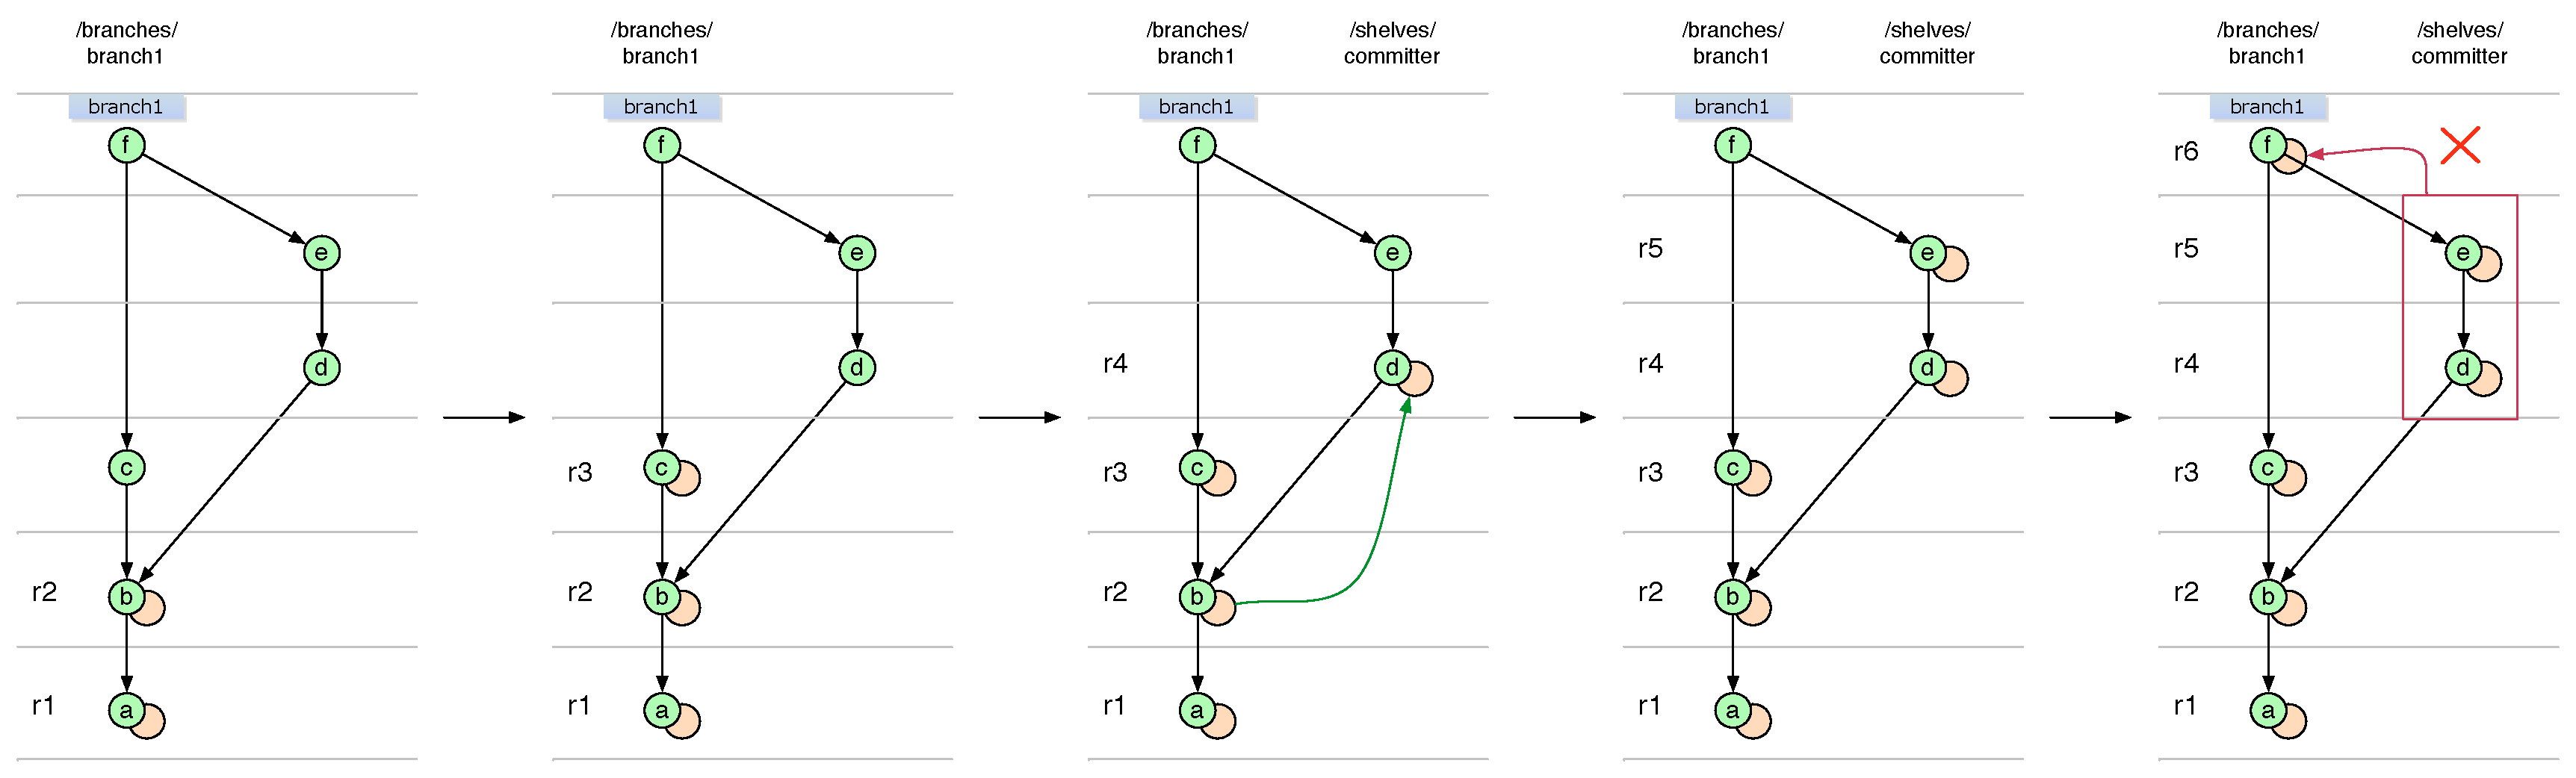
\includegraphics[width=\textwidth]{img/diagrams/boat_merge_git_to_svn.pdf}%
\captionof{figure}{Merge of anonymous Git branch being translated to a sequence of Subversion revisions.}
\label{boat_merge_git_to_svn}%
\end{center}

\subsubsection{Nested Merge}

On Git merge commits translation, Translator might encounter Git merge commit which refer to the parent commit, which,
in its turn, refers to another merge commit.
\\\\
Subversion svn:mergeinfo property which have to be translated to a Git merge commit, might refer to the multiple branches,
either directly enumerating all branches and revisions, or indirectly, by referring to the branch which has svn:mergeinfo property set on it referring to another branch.
\\\\
Above are examples of the \emph{nested merges}. On translating of such merges, Translator takes into account both
directly and indirectly referenced changes and performs translation accordingly to the composite set of the 
changes referenced by the merge commits or by the svn:mergeinfo properties.
\\\\
Shown below are examples of the nested merges translation.
\\\\
The first use case depicted at diagram \ref{nested_merge_full_mergeinfo_git_to_svn}. 
Commit \emph{i} is the merge commit of branches branch3 and branch1. 
But branch1 has a commit \emph{f} which is commit merged branch2 into branch1. 
For that case at corresponding revision r9 we add svn:mergeinfo property to branch3 which includes the merge history of all commits being merged at commit \emph{i}.

\begin{center}
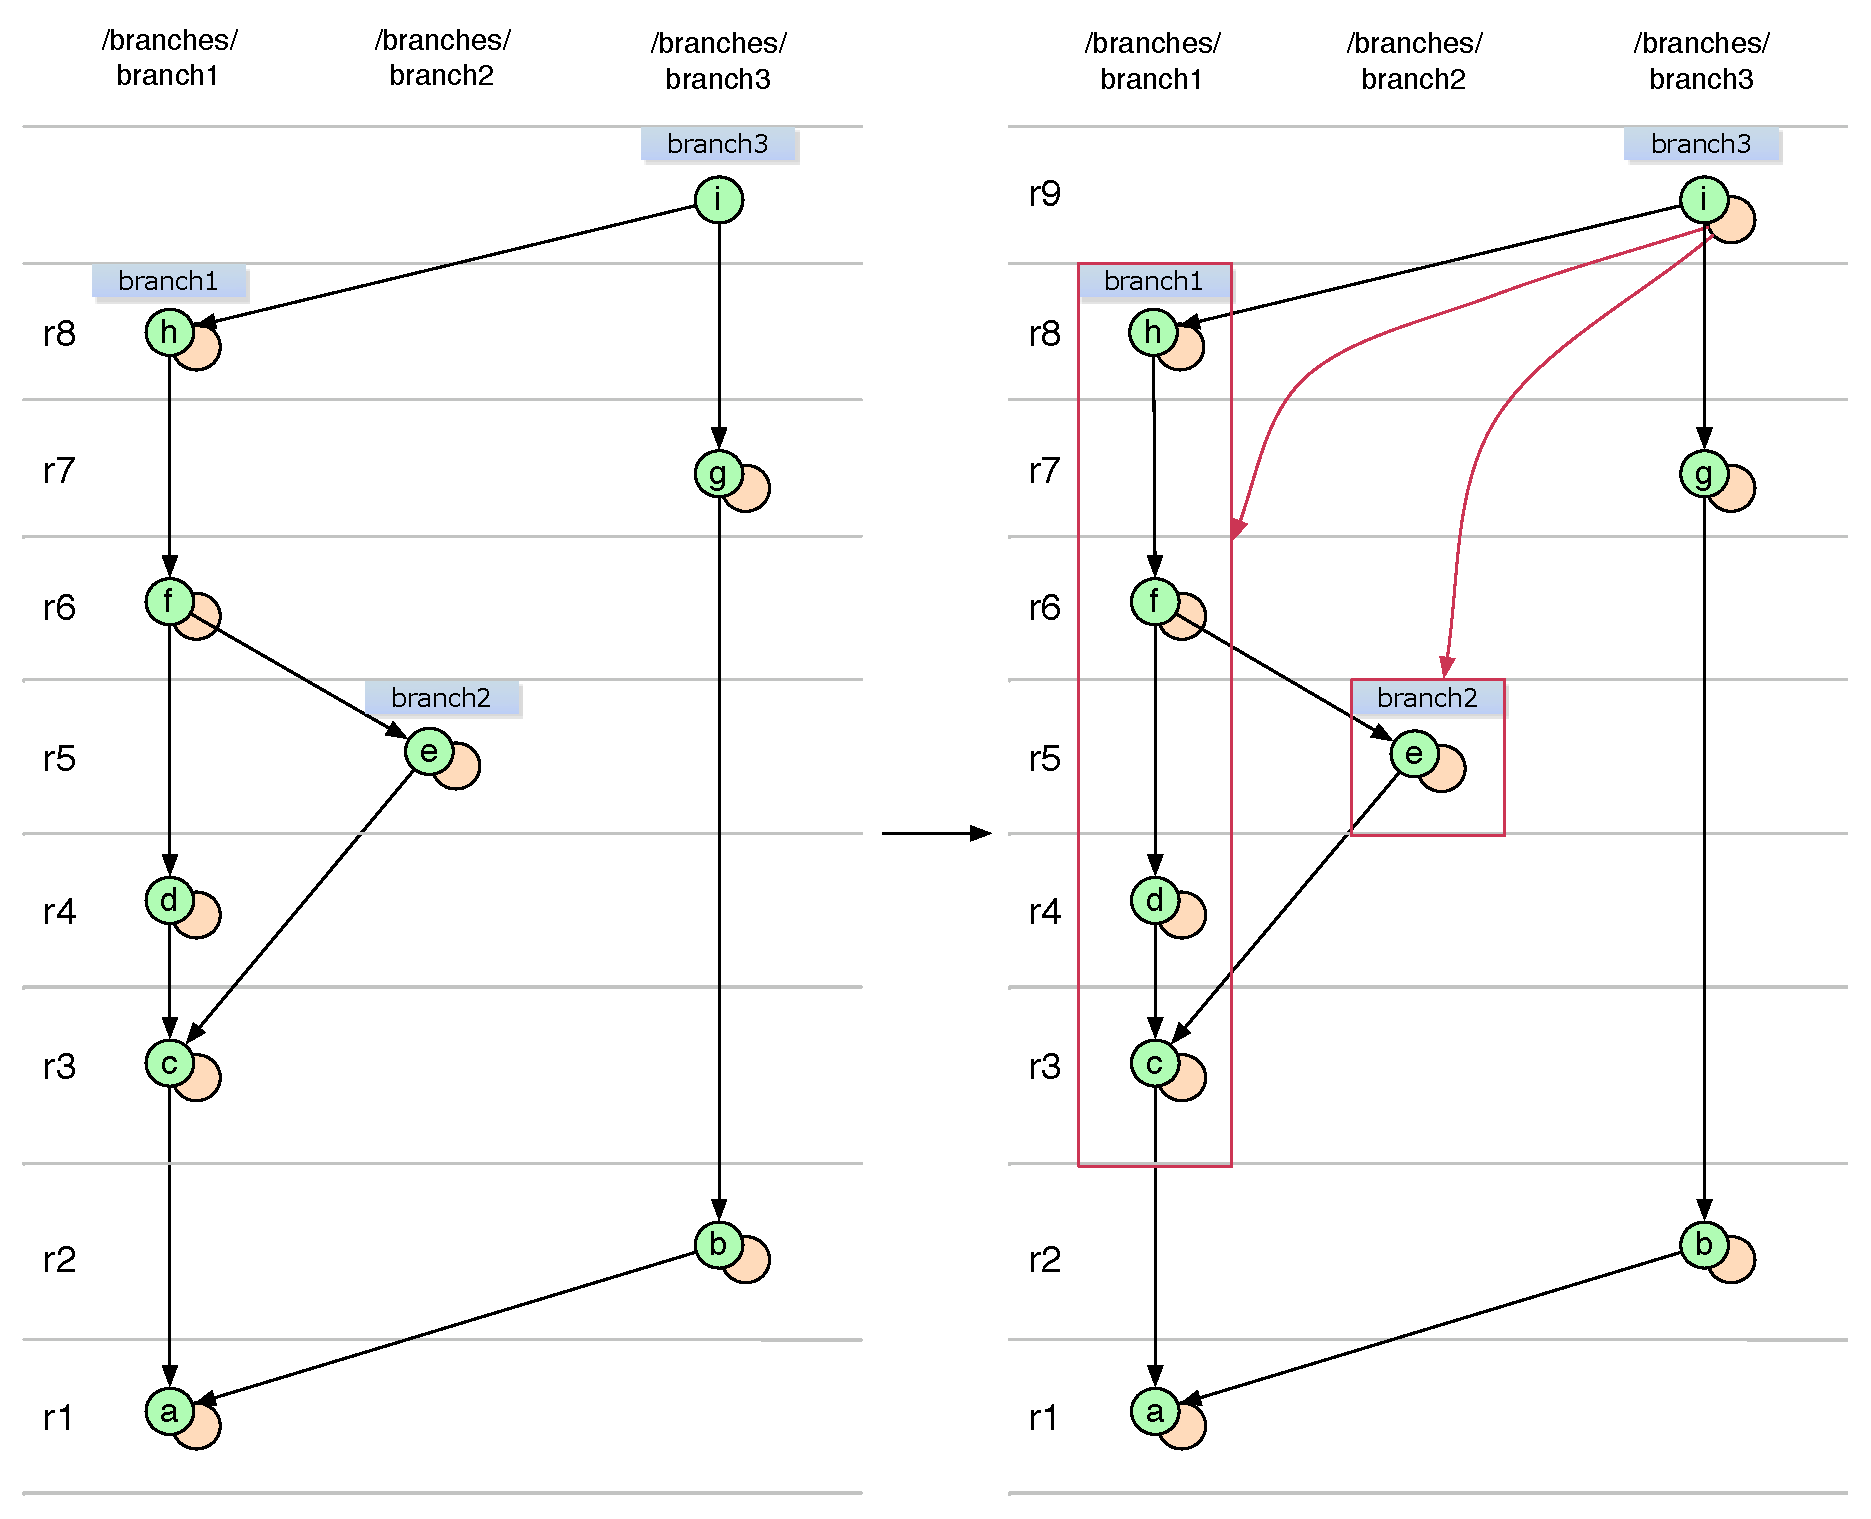
\includegraphics[width=\textwidth]{img/diagrams/nested_merge_full_mergeinfo_git_to_svn.pdf}%
\captionof{figure}{Merge of Git branch which is available from another branch being translated to a sequence of Subversion revisions.}
\label{nested_merge_full_mergeinfo_git_to_svn}%
\end{center}

The mirror of this use case is depicted at diagram \ref{nested_merge_full_mergeinfo_svn_to_git}. Subversion user merged all the revision which represent the whole history of Git commits being merged at commit \emph{i}.

\begin{center}
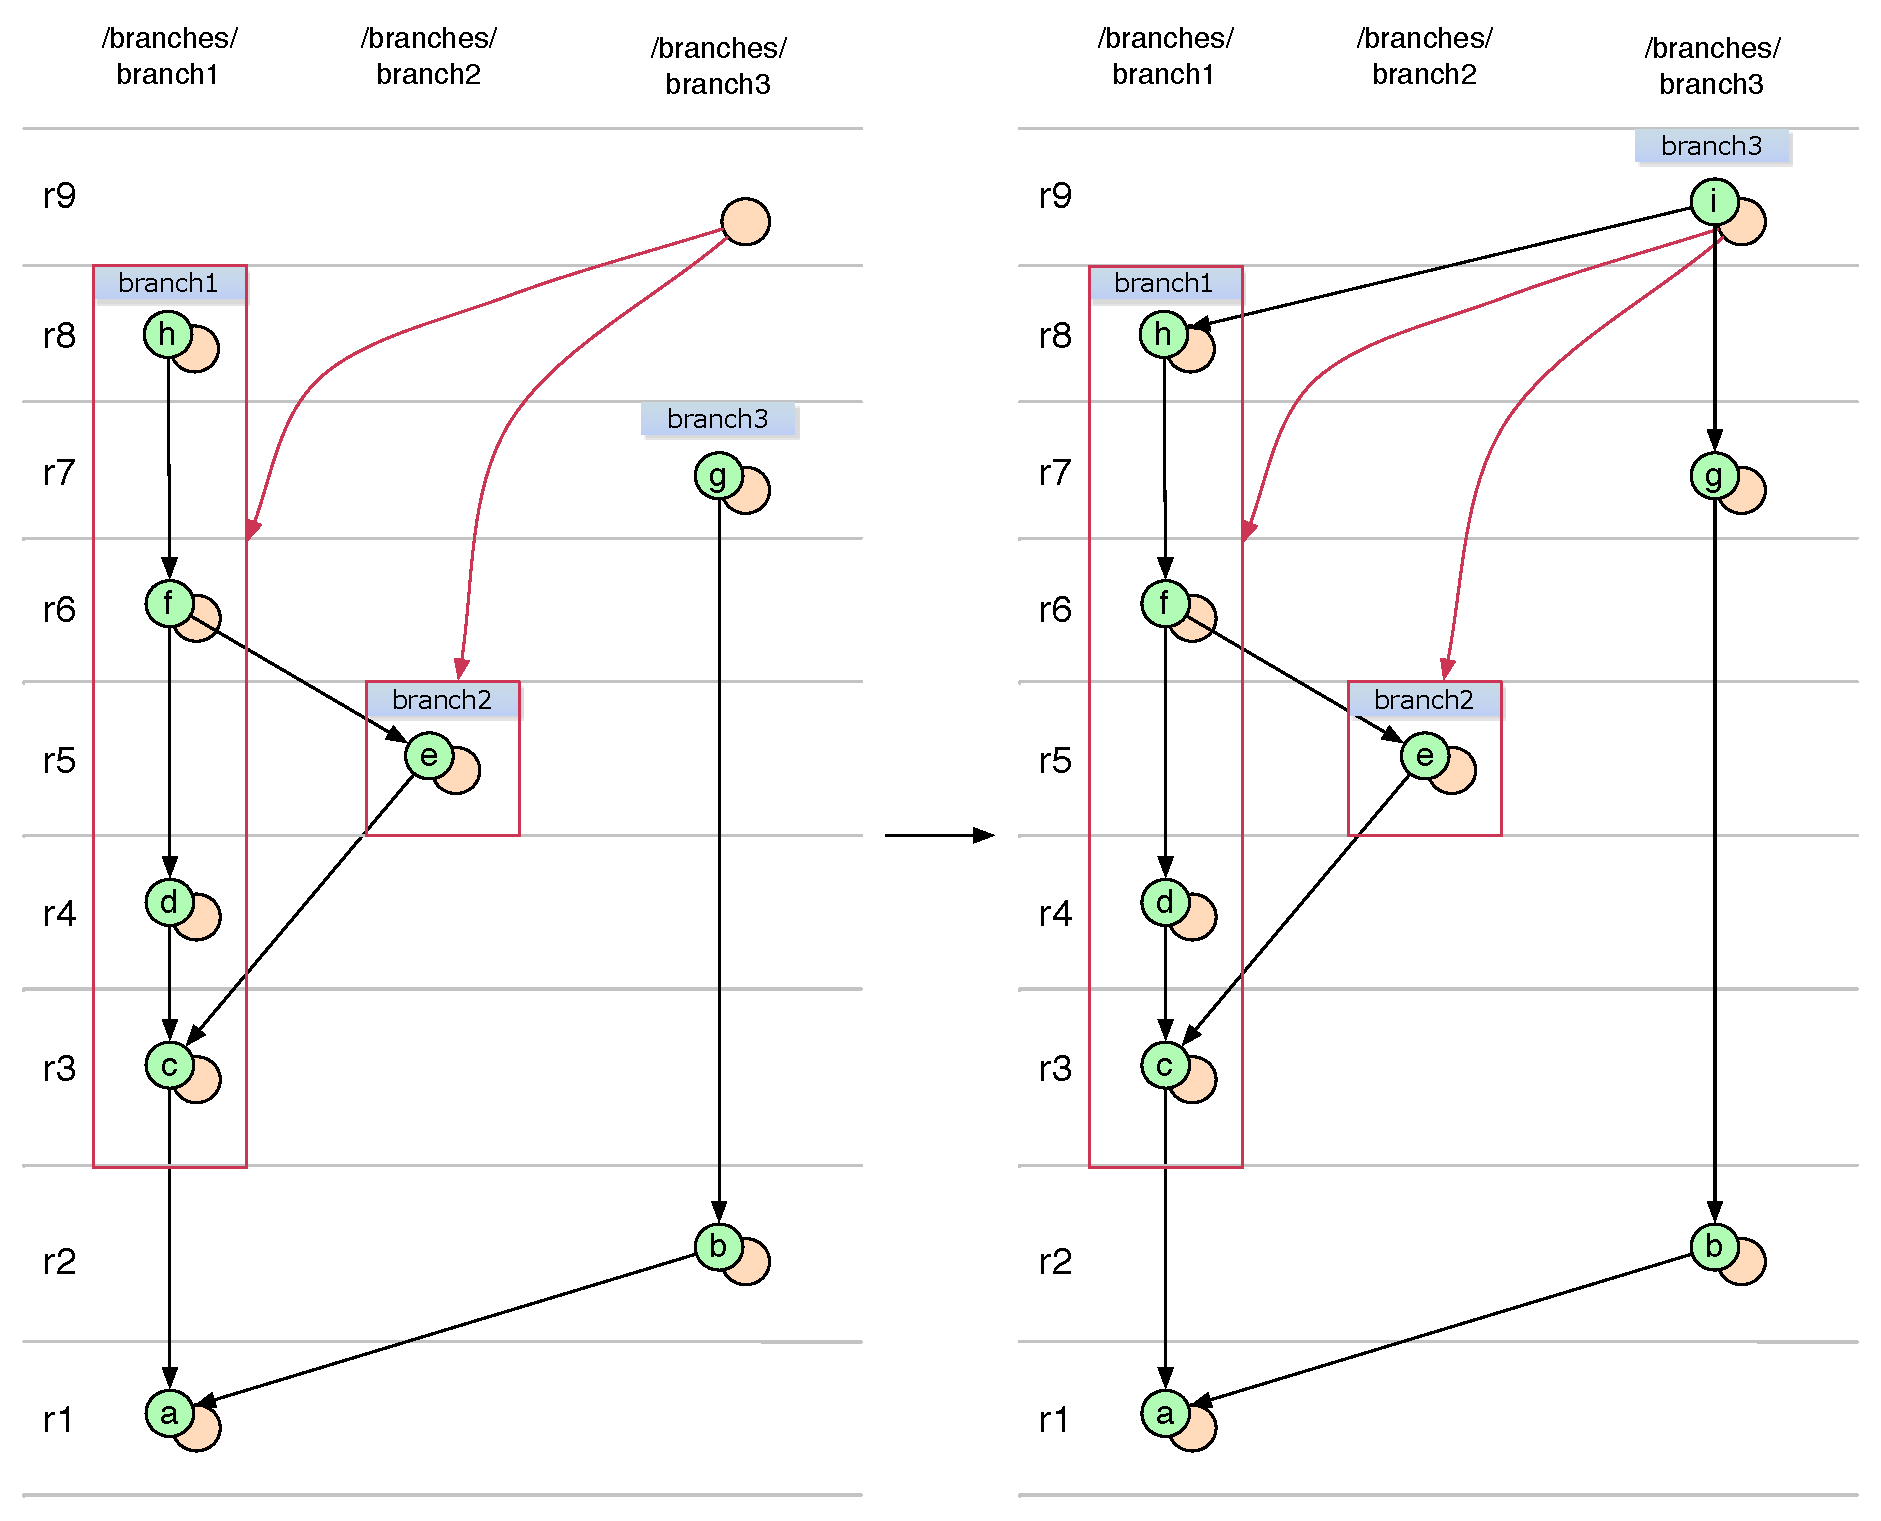
\includegraphics[width=\textwidth]{img/diagrams/nested_merge_full_mergeinfo_svn_to_git.pdf}%
\captionof{figure}{Merge of Git branch which is available from another branch being translated to a sequence of Subversion revisions.}
\label{nested_merge_full_mergeinfo_svn_to_git}%
\end{center}

Slightly modified scenario is depicted at diagram \ref{nested_merge_partly_mergeinfo_svn_to_git}. Subversion user didn't include /branches/branch2@r5 into merge history explicitly. But this change already included via revision /branches/branch1@r6, thus commit \emph{e} is included into merge history of revision r9 implicitly. As result Translator is able to create commit \emph{i} corresponding to revision r9 and set two parents to it.

\begin{center}
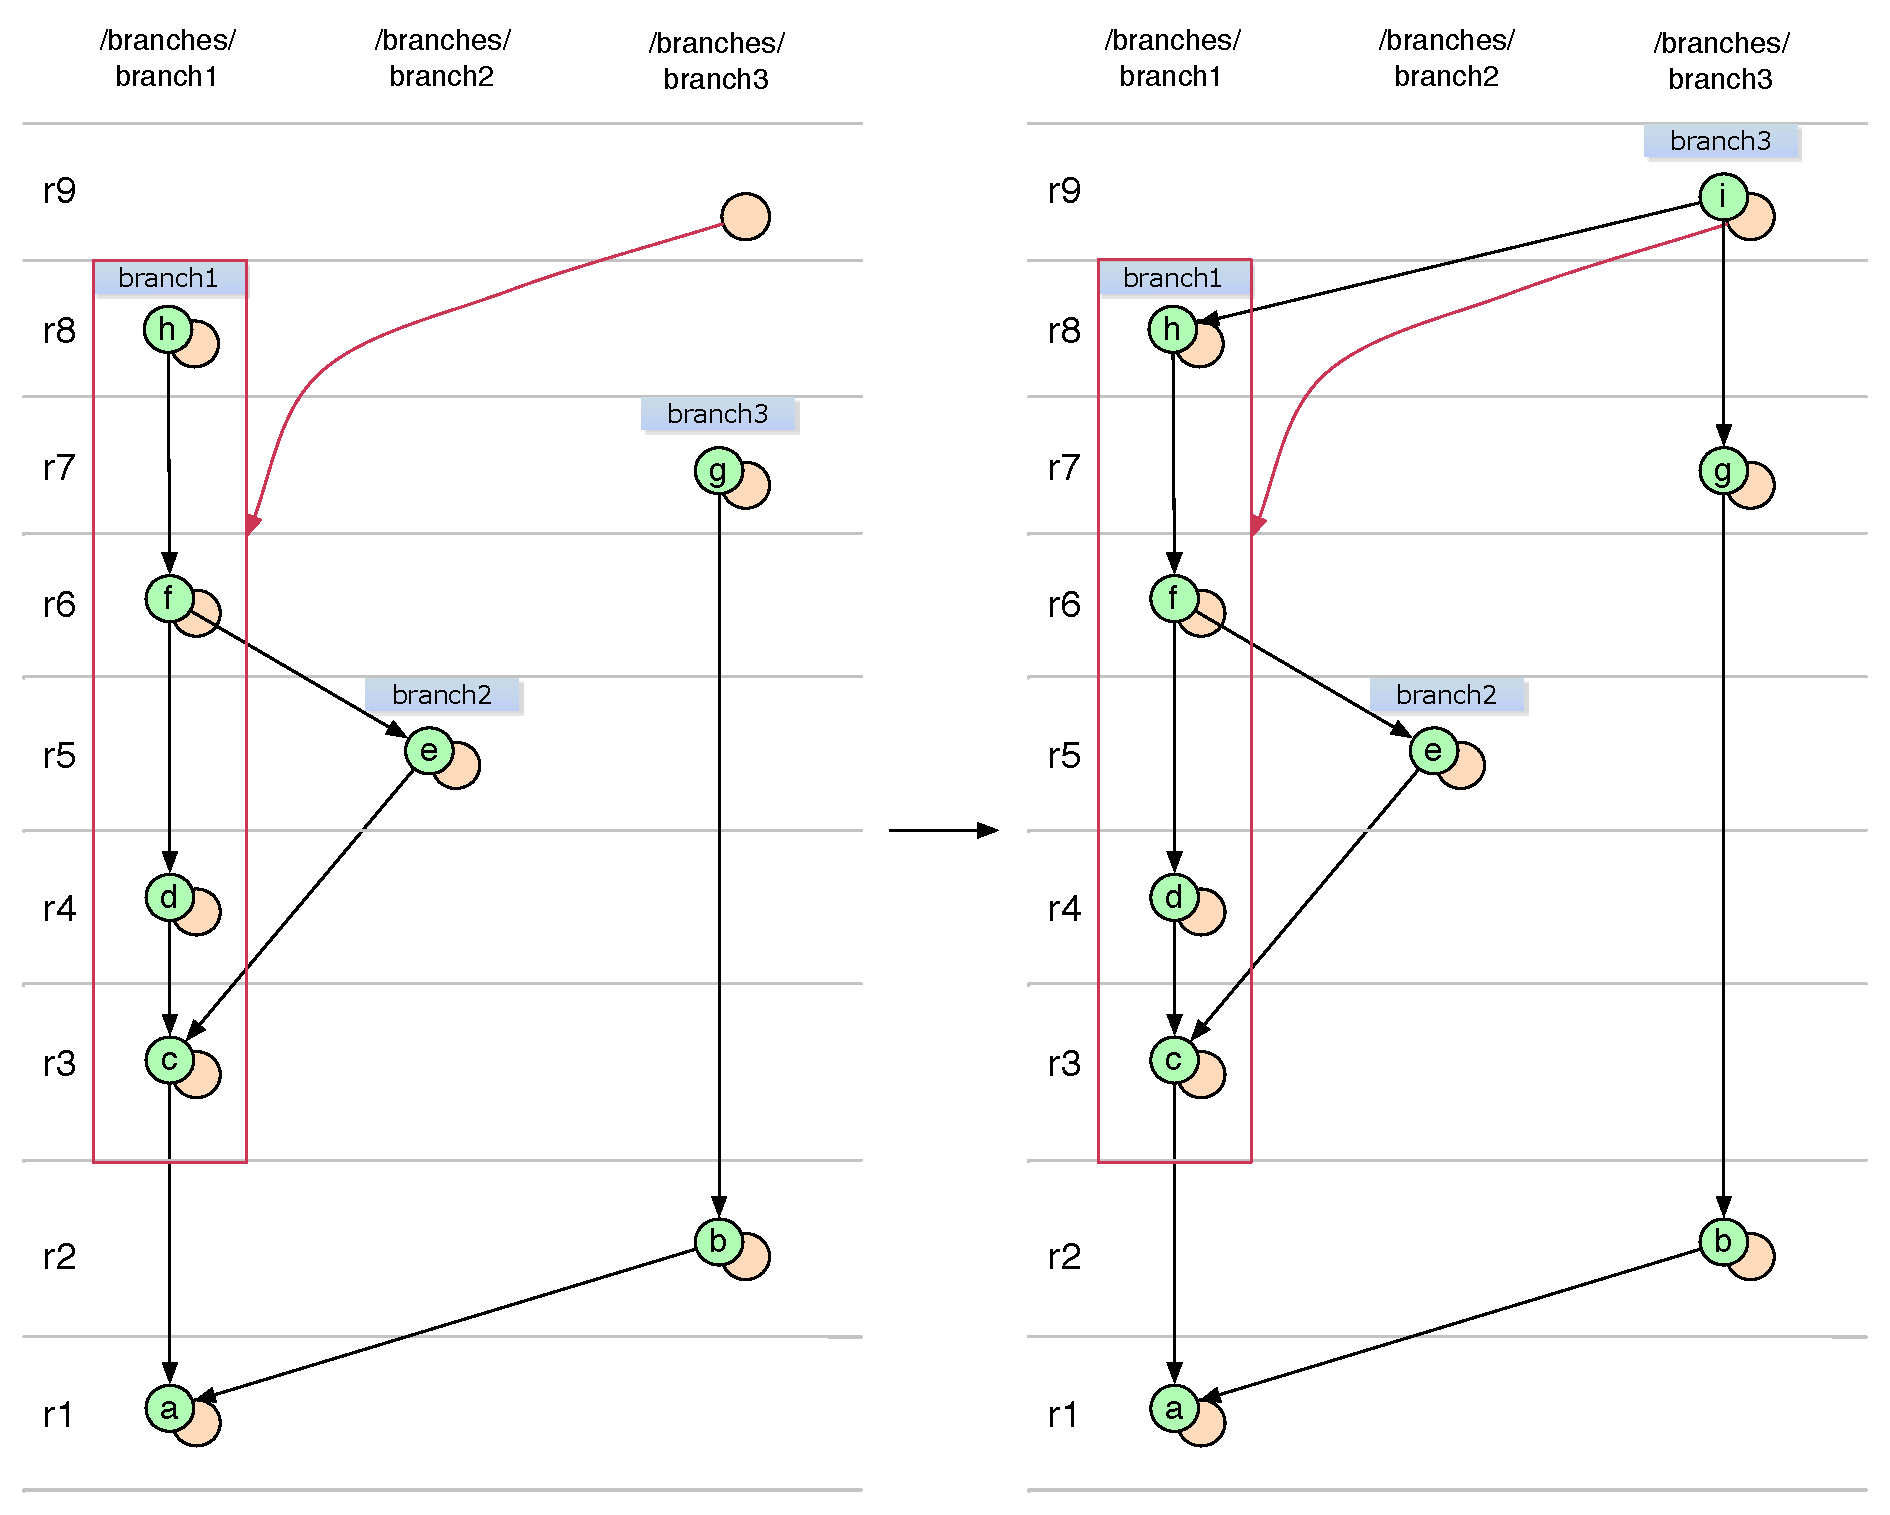
\includegraphics[width=\textwidth]{img/diagrams/nested_merge_partly_mergeinfo_svn_to_git.pdf}%
\captionof{figure}{Merge of Git branch which is available from another branch being translated to a sequence of Subversion revisions.}
\label{nested_merge_partly_mergeinfo_svn_to_git}%
\end{center}

During Git to Subversion translation of merge commits Translator adds to svn:mergeinfo property all the revisions corresponding to commits appended to the history of branch by the merge. Another example of this translation introduced at diagram \ref{merge_sequence_git_to_svn}.

\begin{center}
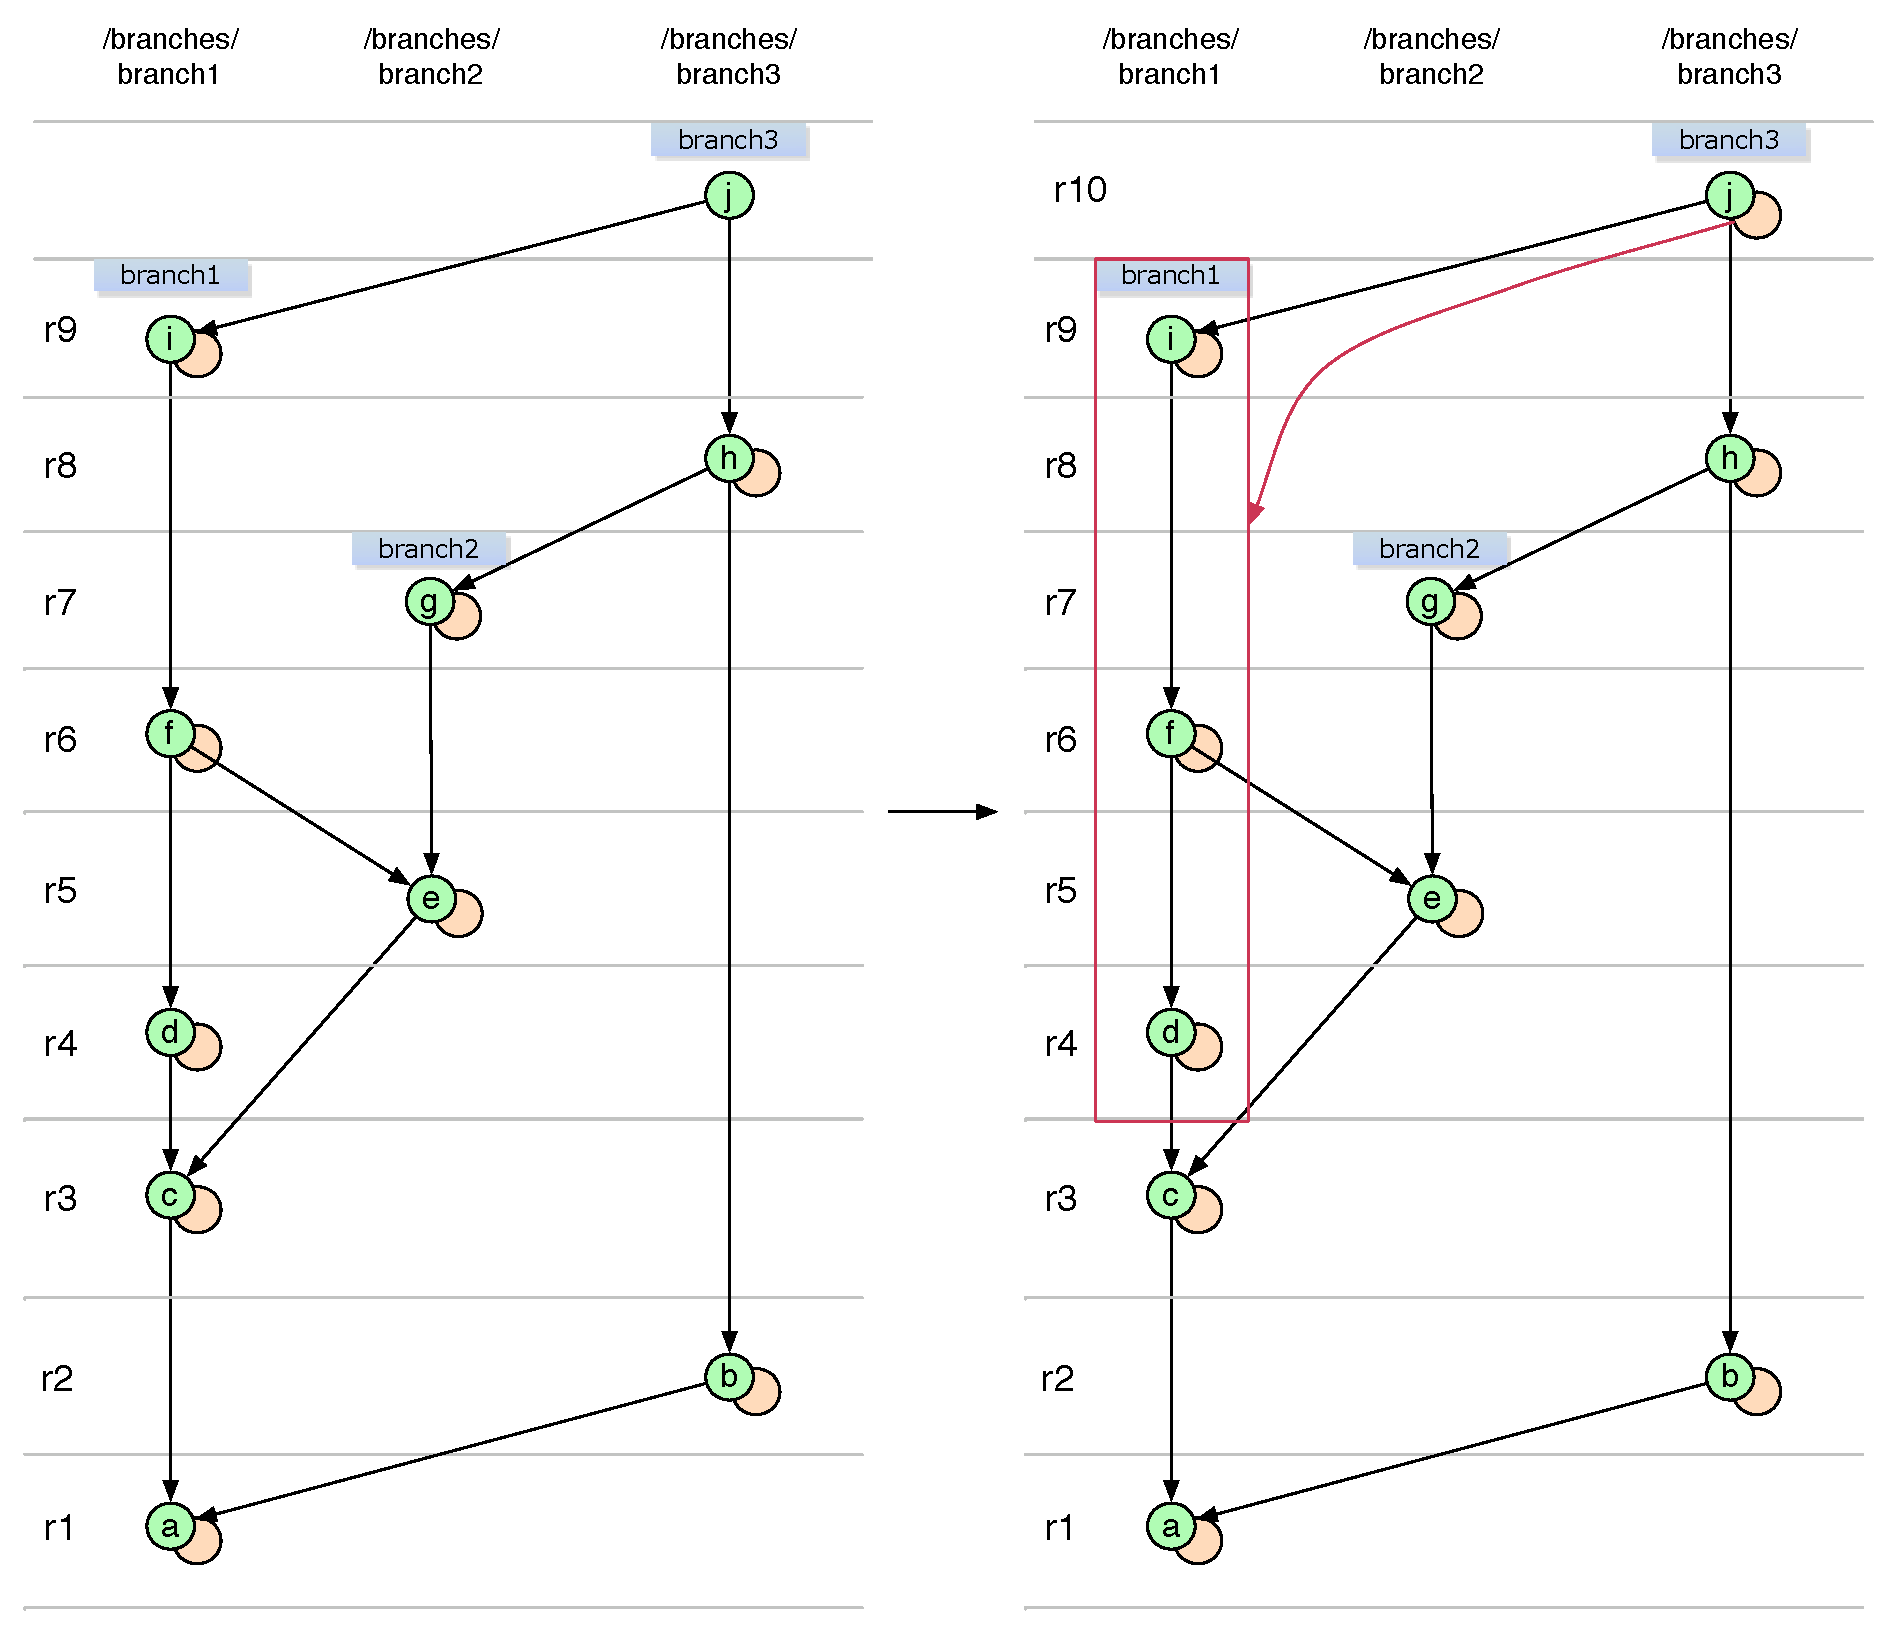
\includegraphics[width=\textwidth]{img/diagrams/merge_sequence_git_to_svn.pdf}%
\captionof{figure}{Merge of Git branch which is available from another branch being translated to a sequence of Subversion revisions.}
\label{merge_sequence_git_to_svn}%
\end{center}

The same holds in opposite direction: when Subversion user merged revisions corresponding to commits which appended to the branch close the history of the branch, Translator creates merge commit which represents this change. This scenario is depicted at diagram \ref{merge_sequence_svn_to_git}.

\begin{center}
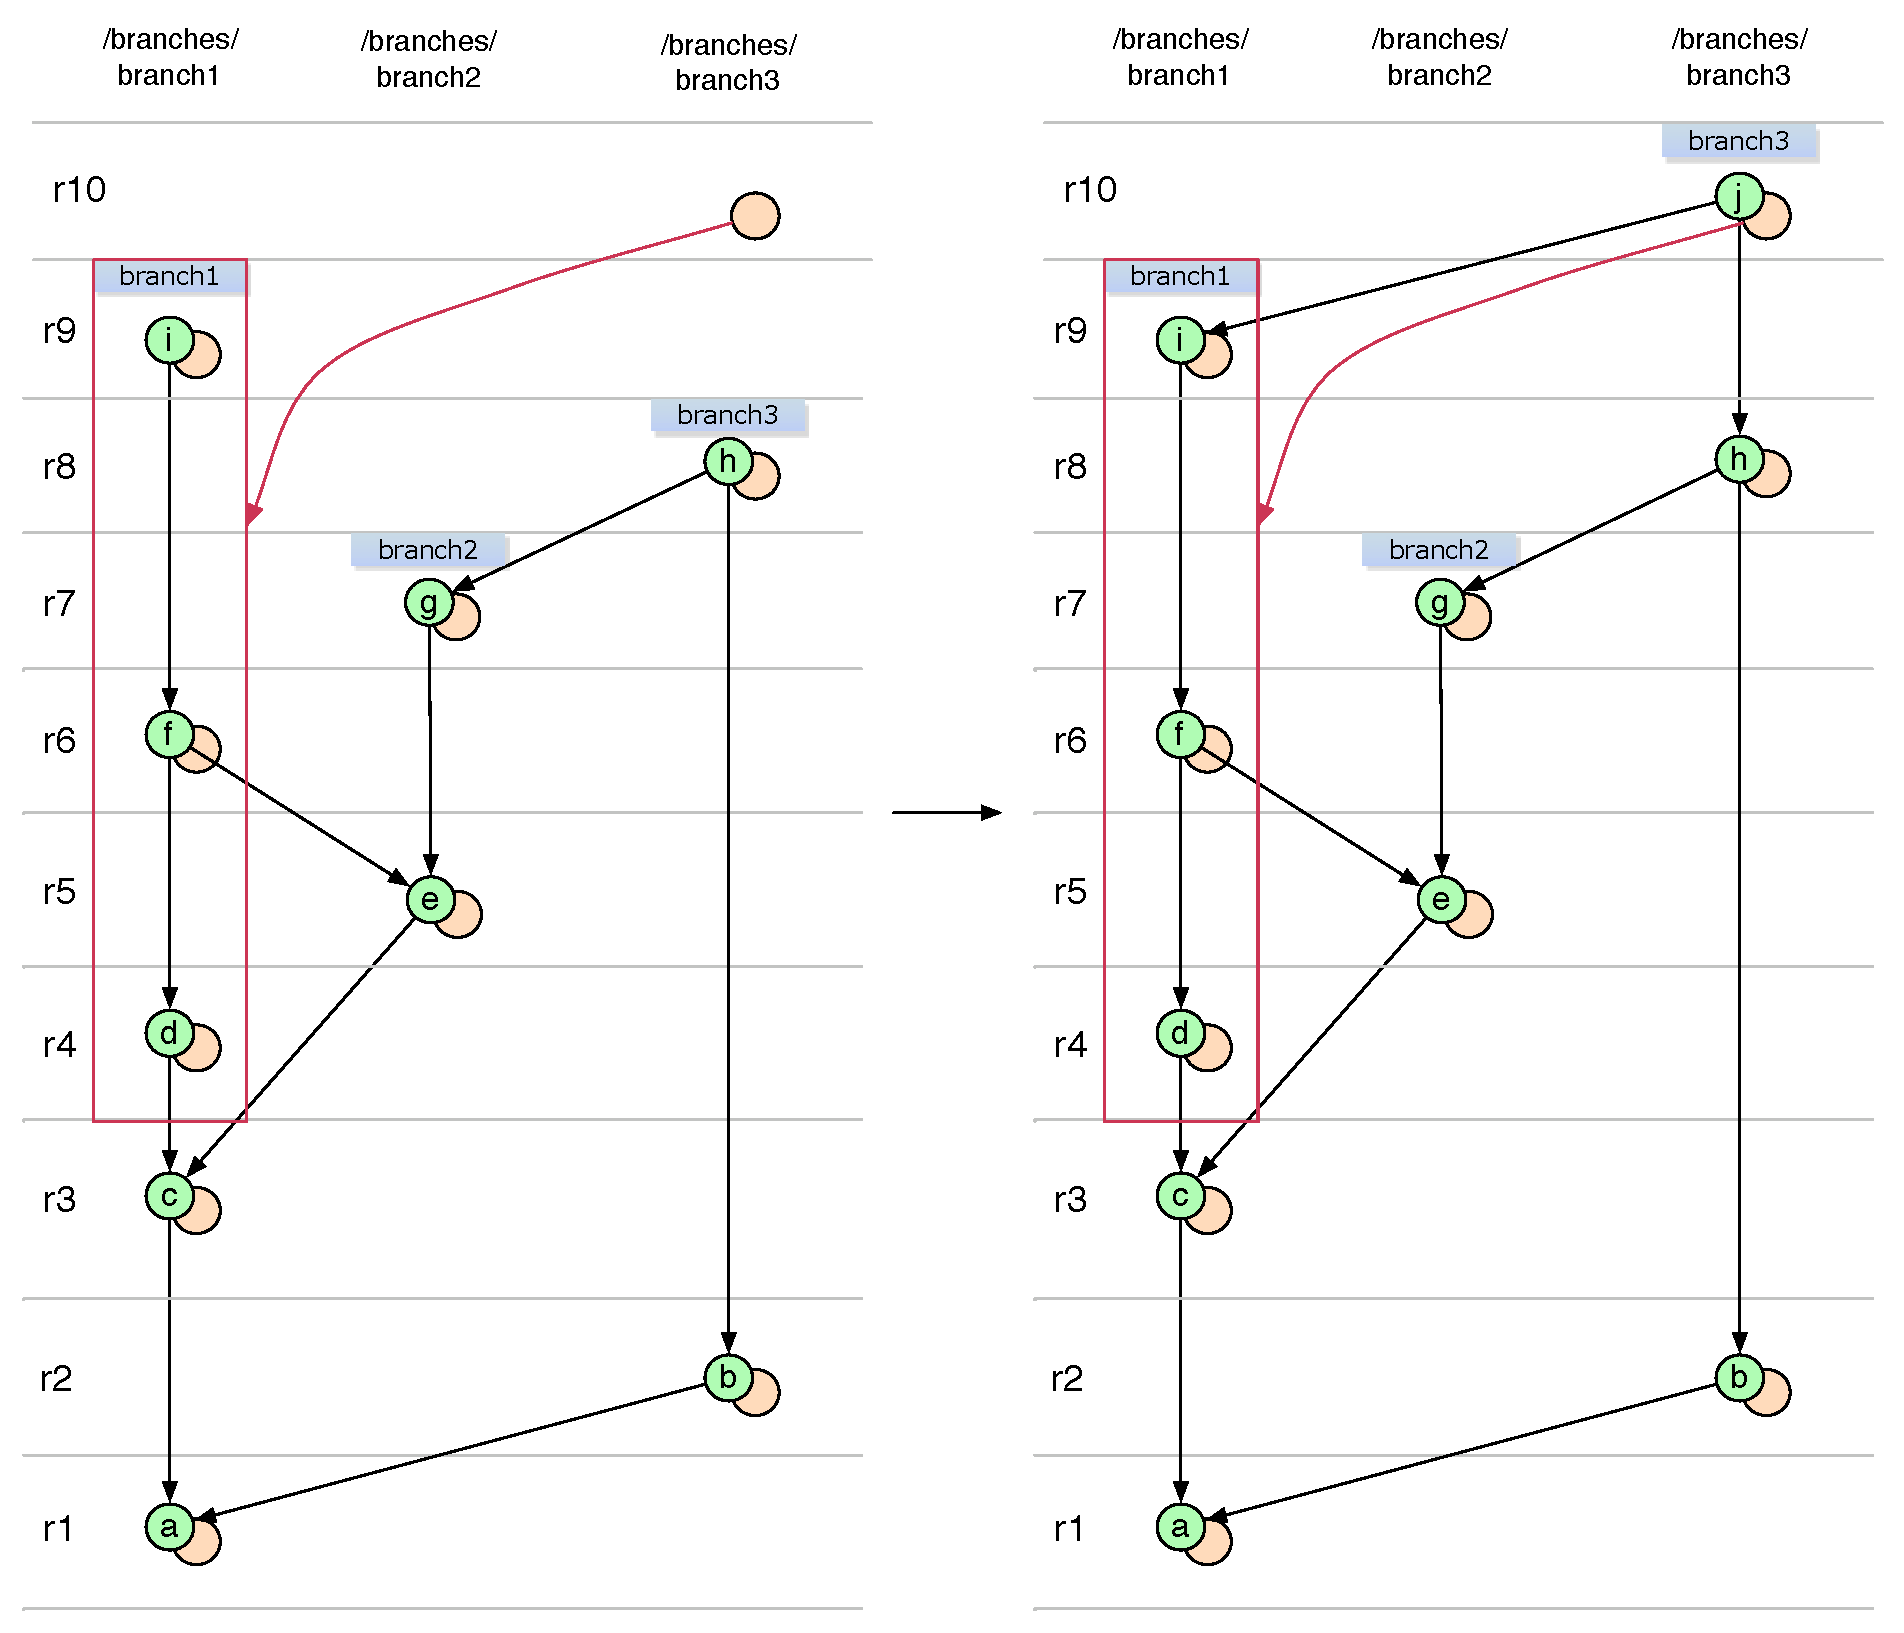
\includegraphics[width=\textwidth]{img/diagrams/merge_sequence_svn_to_git.pdf}%
\captionof{figure}{Merge of Git branch which is available from another branch being translated to a sequence of Subversion revisions.}
\label{merge_sequence_svn_to_git}%
\end{center}

Merged revisions may not include the whole history of certain branch. It is common case when Subversion user performed cherry-pick. As shown before Translator creates common commit for this case with single parent. This scenario is depicted at diagram \ref{no_merge_commit_cherry_pick_sequence_svn_to_git}.

\begin{center}
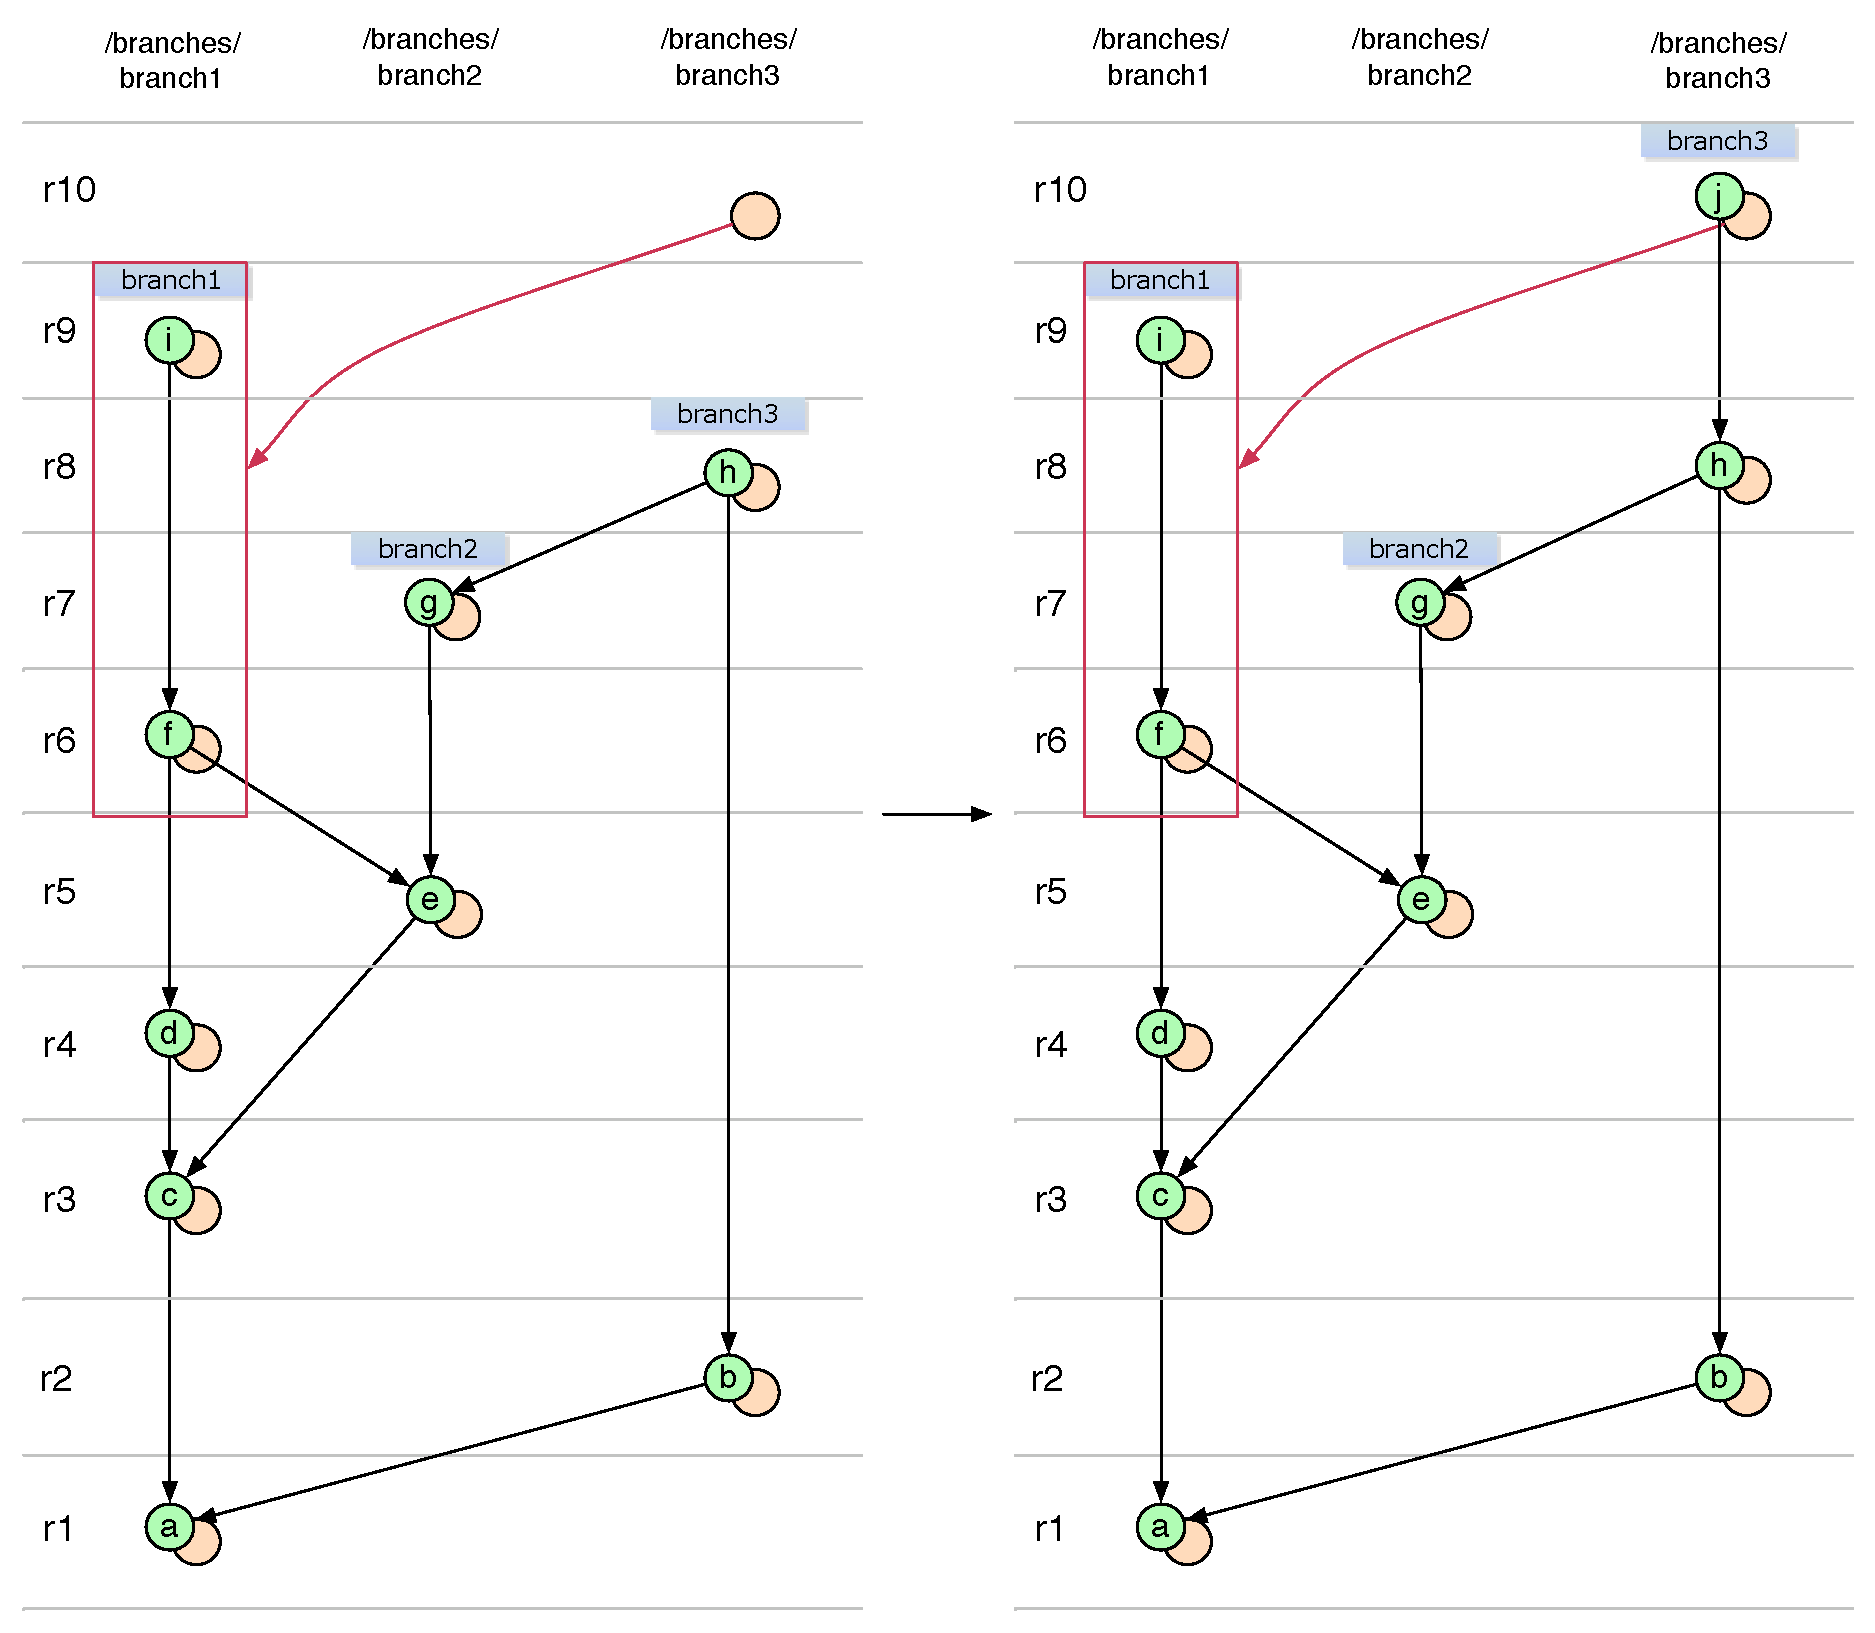
\includegraphics[width=\textwidth]{img/diagrams/no_merge_commit_cherry_pick_sequence_svn_to_git.pdf}%
\captionof{figure}{Merge of Git branch which is available from another branch being translated to a sequence of Subversion revisions.}
\label{no_merge_commit_cherry_pick_sequence_svn_to_git}%
\end{center}

\subsubsection{Octopus Merge}

Both Subversion and Git support so called \emph{octopus merge}, - merge in which an arbitrary number of branches are merged into the target branch in a single revision or commit. 
\\\\
Translator supports this kind of merge in a way shown in the diagrams \ref{octopus_merge_git_to_svn} (for Git to Subversion translation) and \ref{octopus_merge_svn_to_git} (for Subversion to Git translation).

\begin{center}
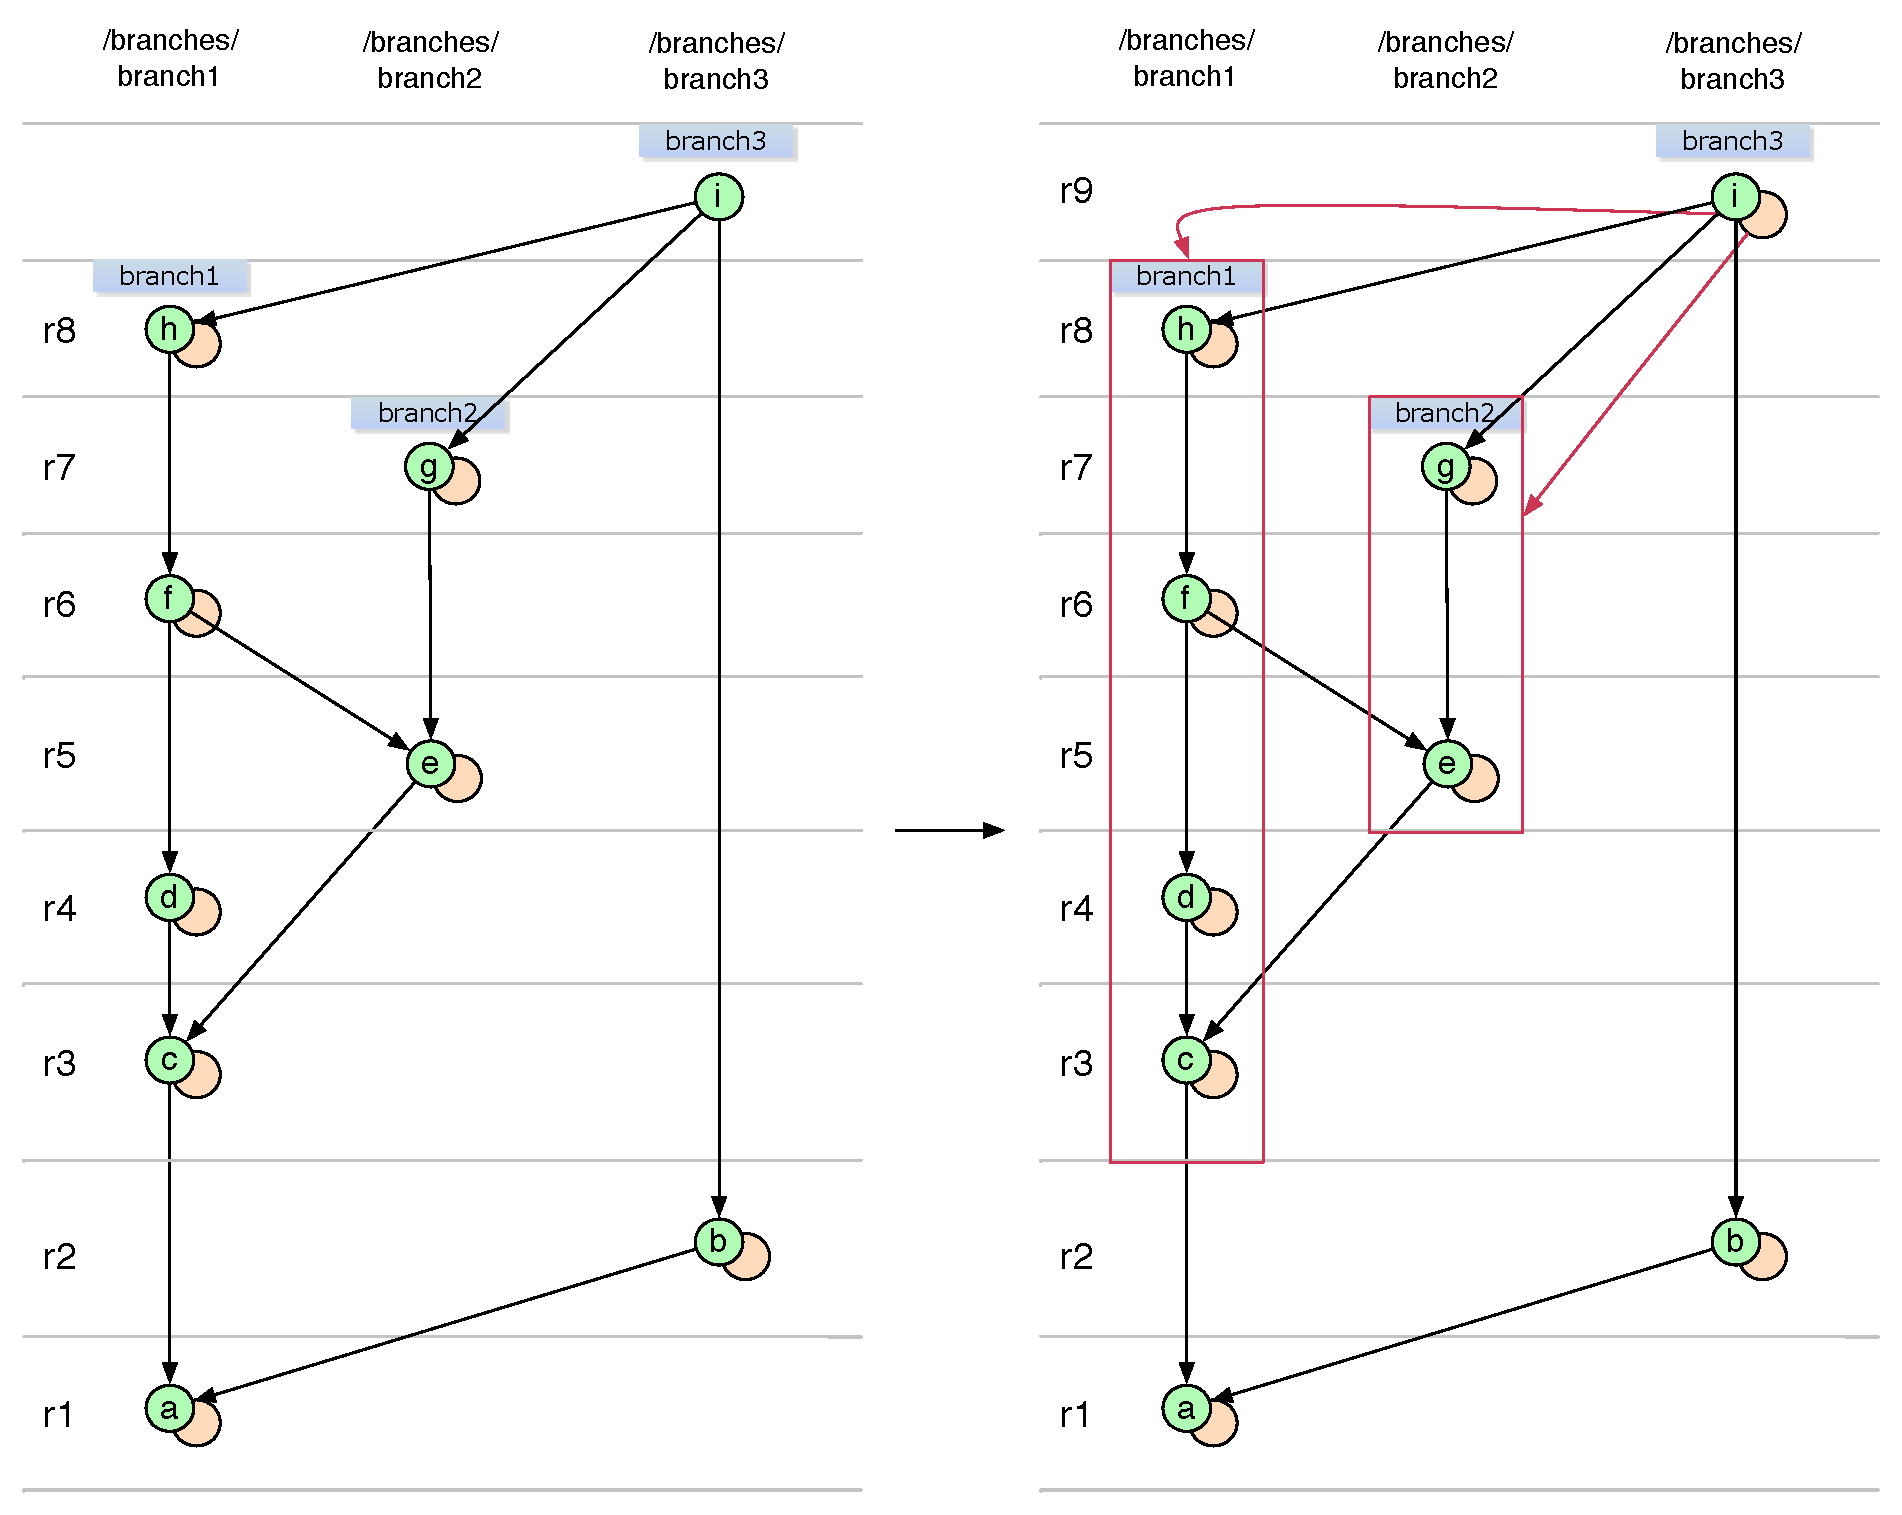
\includegraphics[width=\textwidth]{img/diagrams/octopus_merge_git_to_svn.pdf}%
\captionof{figure}{Octopus merge commit being translated to svn:mergeinfo change.}
\label{octopus_merge_git_to_svn}%
\end{center}

\begin{center}
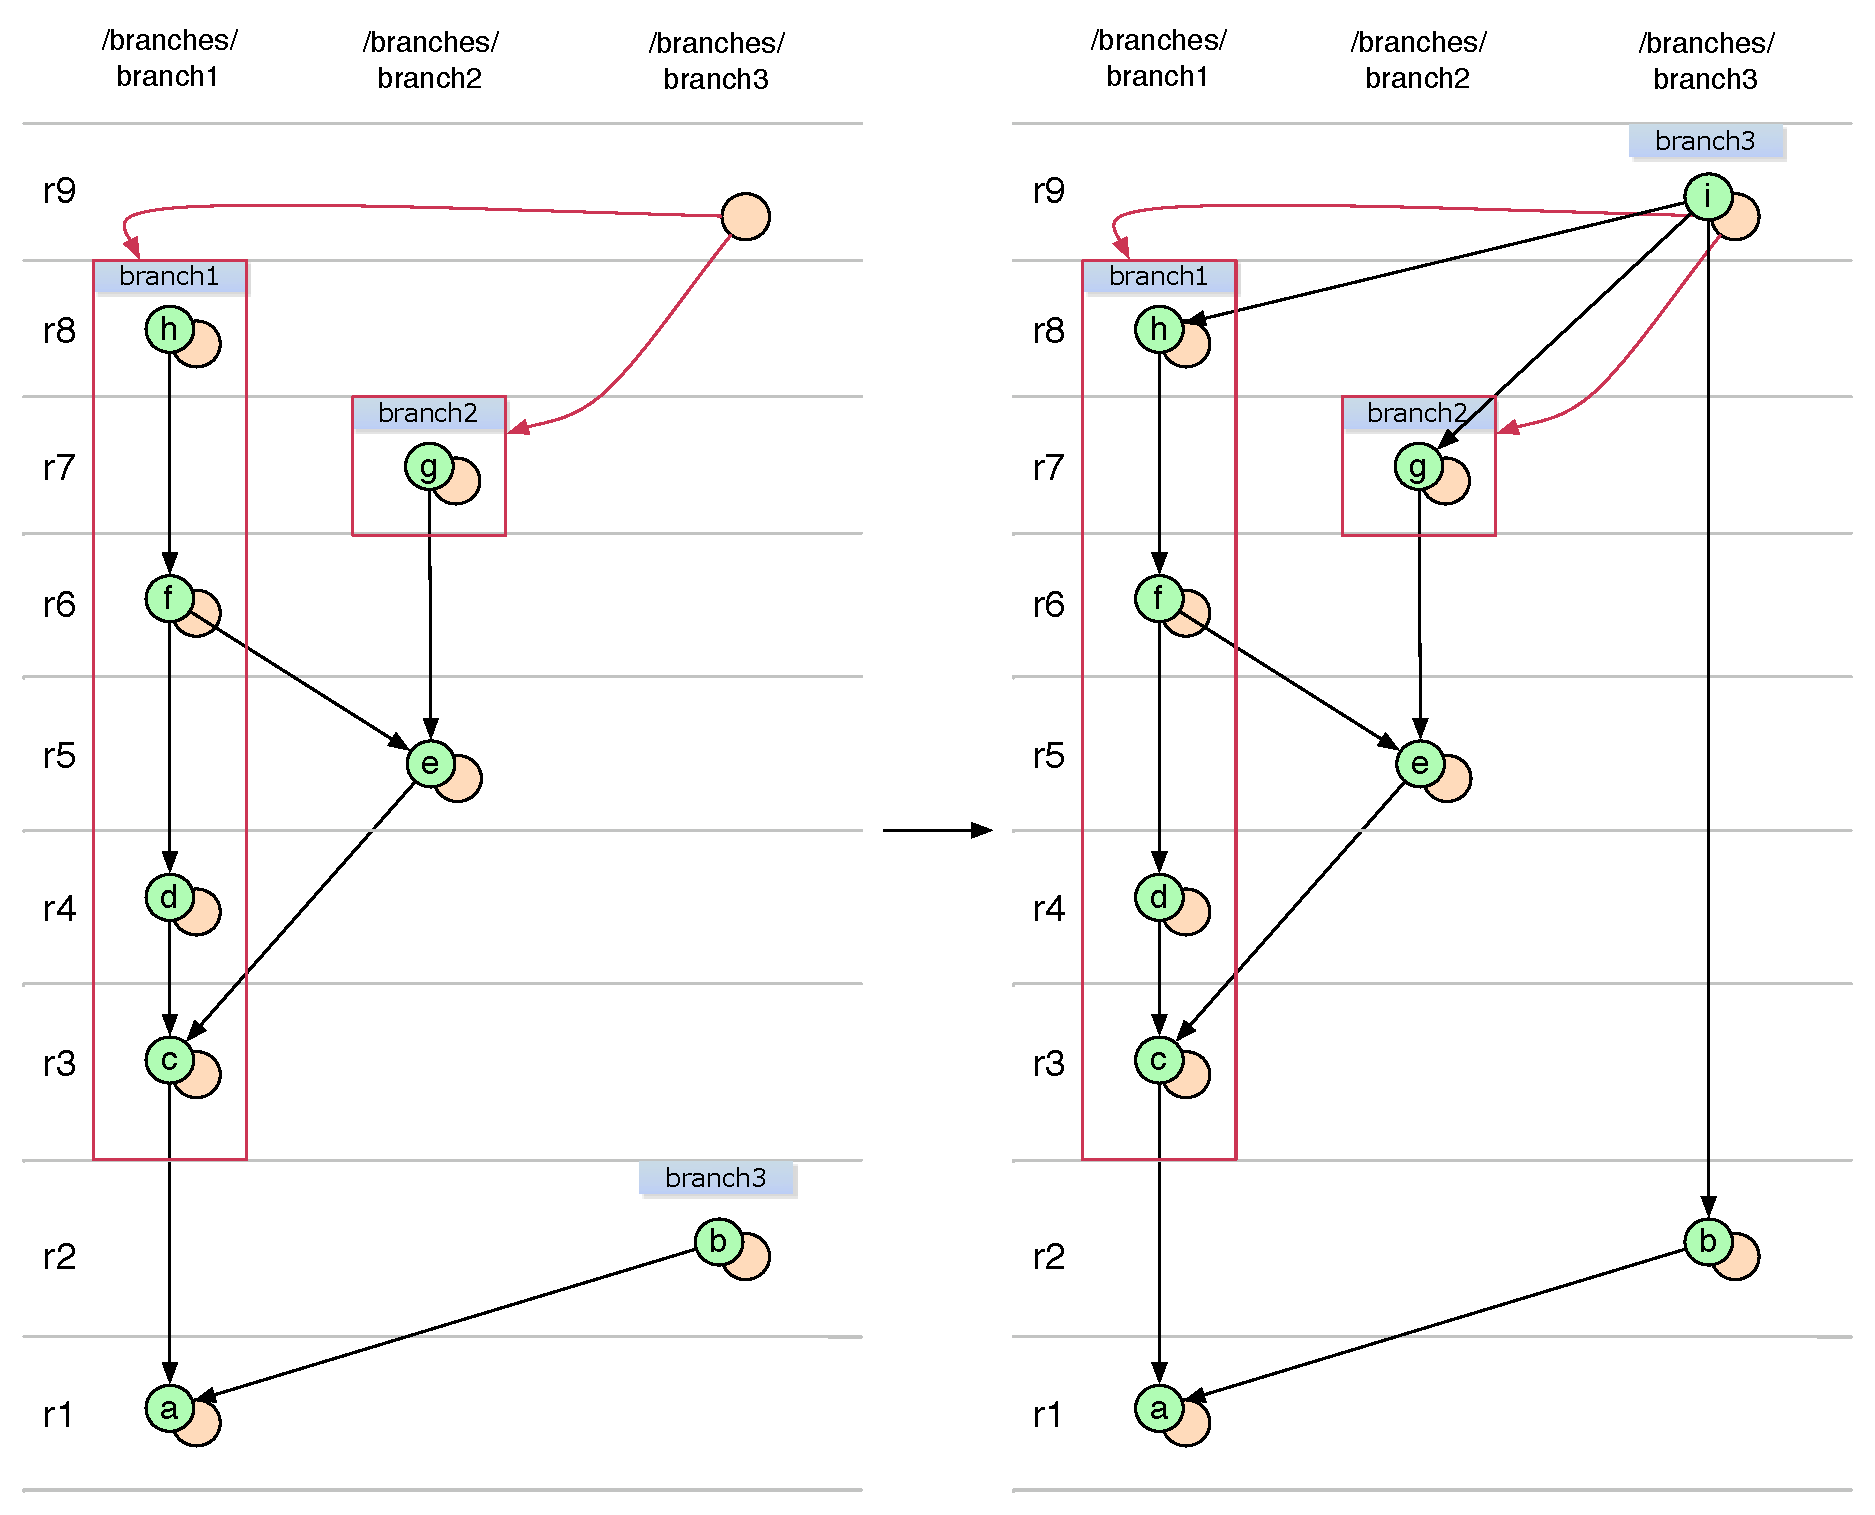
\includegraphics[width=\textwidth]{img/diagrams/octopus_merge_svn_to_git.pdf}%
\captionof{figure}{Change of svn:mergeinfo property being translated to octopus merge commit.}
\label{octopus_merge_svn_to_git}%
\end{center}

\subsection{Copies and Renames}
This section decribes translation of files and directories copies and renames, \emph{other than} copies and renames of 
branches (/branches/\emph{B}) and tags (/tags/\emph{T}). For that sort of copies and renames refer to the "Branches and Tags" 
section of this specification.\\\\
Rename translation does not differ from translation of the copy, because both Git and Subversion
express renames as a composition of copy and deletion. 

\subsubsection{Copies in Subversion to Git}
No special translation is performed for a file or directory copied or renamed in Subversion revision. Copy of the single file is translated 
to creation of a new file in the corresponding Git commit. Copy of a directory is translated to creation of a new directory with all its children
in the corresponding Git commit.

\subsubsection{Copies in Git to Subversion}
Whenever it is revealed that new file in Git commit is a result of copy or rename, this new file creation is translated to a file copy in the 
corresponding Subversion revision.\\\\ 
When amount of copied files in a new directory exceeds certain treshold (percentage of the amount of files in the original directory), then new directory
creation is translated into a directory copy with appropriate directory content adjustment in the correspoding Subversion revision.
\subsection{Properties and Attributes}
Subversion keeps metadata as versioned properties which could be attached to any file or directory under version control. Among these properties there are special ones with \emph{svn:} prefix, Subversion has a number of mechanisms to handle this kind of properties.
\\\\
Git introduces a number of ways to keep metadata:
\begin{enumerate}
\compactlist
\item Every directory and file has \emph{file mode} bytes stored at repository.
\item \emph{.gitignore} file stores file path patterns to be ignored by Git operations.
\item \emph{.gitattributes} is a special format file which could be added into any directory.
\end{enumerate}

Translation of the specified metadata is described in further sections.

\subsubsection{End-of-Line Bytes and MIME Types}
Subversion supports EOL bytes substitution since its early versions. Support of different EOL-styles was introduced in Git at version 1.7.2. Translator is supposed to perform valid EOL translation for users of Git version 1.7.2 or above.
\\\\
EOL substitution makes sense for text files only, so Translator performs translation of both EOL-style and MIME-type metadata. Subversion uses svn:eol-style and svn:mime-type properties for this kind of metadata. Git introduces \emph{eol} and \emph{text} attributes for that purpose. Subversion stores the metadata as property attached to file, but Git keeps attributes in .gitattributes file located at parent directory or higher.
\\\\
If user modified EOL style or MIME type of certain file at Subversion repository, Translator applies this change to the metadata of corresponding file in Git repository. The ultimate goal of Translator for this case is to perform less modifications of .gitattributes files. To achieve that goal translation process has the following steps:

\begin{enumerate}
\compactlist
\item For every file with modified svn:eol-style or svn:mime-type property Translator tries to find a corresponding line in one of .gitattributes files located at parent directory or higher.\\
	
\item If attribute line is found, Translator adjusts corresponding attribute to reflect performed change. Basically Translator adds a line with pattern corresponding to the path of modified file and a new attribute:\\\\

\emph{/$<$relative-file-path$>$ $<$text-related-value$>$ $<$eol-related-value$>$},\\\\

where $<$text-related-value$>$ and $<$eol-related-value$>$ are generated according to the rules specified at table \ref{eol_mime_svn_to_git}.\\
	
\item If no .gitattributes file was found among parent directories of the file, Translator creates a new .gitattributes file at the parent directory of the file with the following content:\\\\

\emph{/$<$file-name$>$ $<$text-related-value$>$ $<$eol-related-value$>$},\\\\

where $<$text-related-value$>$ and $<$eol-related-value$>$ are generated according to the rules specified at table \ref{eol_mime_svn_to_git}.\\
	
\item If a number of .gitattributes files were found at parent directories of the file, the closest one is chosen. Translator appends to this file the following line\\\\

\emph{/$<$relative-file-path$>$ $<$text-related-value$>$ $<$eol-related-value$>$},\\\\

where $<$text-related-value$>$ and $<$eol-related-value$>$ are generated according to the rules specified at table \ref{eol_mime_svn_to_git}.\\

\item Finally for every created or modified .gitattributes file Translator tries to compact added rules using recursive path pattern instead of explicit path pattern.
\end{enumerate}

Note that this approach keeps comments at .gitattributes file unmodified during the translation.

\begin{center}
\begin{tabular}{ | l | l | l | l |}
	\hline
	svn:eol-style &   svn:mime-type &   text  & eol \\ \hline \hline
	-             &   text/-        &   unset & undef \footnotemark[1] \footnotemark[2] \\ \hline
	-             &   binary        &   unset & undef \\ \hline
	lf            &   text/-        &   set   & lf \\ \hline
	lf            &   binary        &   unset & undef \\ \hline
	cr            &   text/-        &   unset & undef  \footnotemark[3] \\ \hline
	cr            &   binary        &   unset & undef \\ \hline
	crlf          &   text/-        &   set   & crlf \\ \hline
	crlf          &   binary        &   unset & undef \\ \hline
	native        &   text/-        &   set   & undef \footnotemark[4] \\ \hline
	native        &   binary        &   unset & undef \\ \hline
\end{tabular}
\captionof{table}{Subversion to Git EOL and MIME translation.}
\label{eol_mime_svn_to_git}
\footnotetext[1]{\emph{undef}, in general, needs only to be set, if there is another rule which matches the file, otherwise we may skip these attributes at all.}
\footnotetext[2]{Missing Subversion properties mean text, leave EOLs as is for that case.}
\footnotetext[3]{Subversion recognizes CR EOL-style, Git does not.}
\footnotetext[4]{svn:eol-style property value \emph{native} should stay the same, Git user may configure \emph{native} via \emph{core.eol} configuration property.} 
\end{center}

Note that Git user should set \emph{core.eol} configuration parameter to allow correct handling of \emph{native} value of svn:eol-style property.
\\\\
Once Git user modified one of .gitattributes files, Translator performs the following steps to apply changes to the metadata of corresponding files in Subversion repository:

\begin{enumerate}
\compactlist
\item For every file affected by the change new svn:eol-style and svn:mime-type properties are calculated.\\
\item If new properties and the properties before the change don't differ, Translator performs no further actions.\\
\item If for every modified property one of its values was \emph{undef}, Translator performs no further actions.\\
\item Otherwise Translator attaches new properties to affected files.\\
\end{enumerate}

Note also that if Subversion repository contains .gitattributes file, its content is inaccessible from the Git repository.

\begin{center}
\begin{tabular}{ | l | l | l | l |}
	\hline
	text  & eol      &  svn:eol-style  &  svn:mime-type \\ \hline
	unset & undef    &  -              &  -/binary \footnotemark[1] \\ \hline
	unset & unset    &  -              &  -/binary \footnotemark[2] \\ \hline
	unset & set      &  native         &  - \footnotemark[3] \\ \hline
	unset & lf       &  lf             &  - \\ \hline
	unset & crlf     &  crlf           &  - \\ \hline
	set   & undef    &  native         &  - \\ \hline
	set   & unset    &  native         &  - \footnotemark[4] \\ \hline
	set   & set      &  native         &  - \\ \hline
	set   & lf       &  lf             &  - \\ \hline
	set   & crlf     &  crlf           &  - \\ \hline
	auto  & undef    &  native/-       &  -/binary \footnotemark[1] \\ \hline
	auto  & unset    &  native/-       &  -/binary \footnotemark[5] \\ \hline
	auto  & set      &  native/-       &  -/binary \\ \hline
	auto  & lf       &  lf/-           &  -/binary \\ \hline
	auto  & crlf     &  crlf/-         &  -/binary \\ \hline
\end{tabular}
\captionof{table}{Git to Subversion EOL and MIME translation.}
\label{eol_mime_git_to_svn}
\footnotetext[1]{Perform binary check.}
\footnotetext[2]{unset/unset is redundant, treat it like unset/undef.}
\footnotetext[3]{From Git documentation:\\eol - This attribute sets a specific line-ending style to be used in the working directory. It enables end-of-line normalization without any content checks, effectively setting the text attribute.}
\footnotetext[4]{set/unset is contradiction, but text has precedence over eol, hence treat like set/undef.}
\footnotetext[5]{auto/unset is contradiction, but text has precedence over eol, hence treat like auto/undef}
\end{center}

\subsubsection{Symbolic Links}
Git stores symbolic link as an entry at Tree Object with a special file mode and corresponding blob containing \emph{path/to/target}.
\\\\
Subversion represents symbolic link as a file with content \emph{link path/to/target} and a property svn:special set on it.
\\\\
So translation is performed by adding or removing \emph{link } prefix to the file content and setting the mode or the property.
\\\\
If file at Subversion repository has svn:special property but its content doesn't start with \emph{link } prefix, it is considered as an ordinary file and translated as a blob.
\subsubsection{Executables}
In Git repository, exectuable files are marked with a special file mode. Executable file in Subversion repository keeps svn:executable property. 
Thus, svn:executable property is translated into Git file mode and vice versa directly.
\subsubsection{Ignores}

For files excluded from version control Subversion and Git introduce \emph{ignores} concept.
\\\\
Subversion user may set svn:ignore property on an arbitrary directory with a list of file name patterns as property value. Corresponding files will be ignored inside this directory.
\\\\
Git user may add a .gitignore file to version control and add a list of file path pattern to be ignored at directory and its children recursively.

\subsubsection{Subversion Externals and Git Submodules}
Translation of Subversion External to Git Submodule and vice versa is straightforward, 
when Git repository referred by the submodule is hosted on GitHub or when Subversion svn:external property refers 
to the branch of the repository hosted on the GitHub.
\\\\
Subversion external properties referring to third-party repositories, or to the non-branch directories of the GitHub Subversion repositories as
well as any file externals are left untranslated.
\\\\
Git submodules referring to the third-party repositories are left untranslated.

\subsection{Git Forks}
Git Fork is an unique feature of GitHub. First version of Translator translates Git Fork and pull request using Subversion concepts of copy and merge,
but makes not attempt to represent Subversion operations as a Git Fork.\\\\
Further versions of Translator might extend translation
rules so that some specific copies and merges performed in Subversion repository are translated into Git Fork.

\subsubsection{Forked Repository}
Git Repository Fork creates new Git repository on GitHub. This new forked Git repository has the following 
important features:
\begin{itemize}
\item Repository is assigned to a particular \emph{user}
\item Repository holds information on its \emph{origin} and includes complete origin history
\item Changes made in the forked repository might be \emph{pulled back} into origin repository
\end{itemize}

These features make its natural to translate Git Fork into a copy \emph{within} Subversion repository. Single fork 
operation is translated into a revision which copies Subversion repository top-level directories into another top-level directory. 
Thus, fork performed by the \emph{user} will be translated into the following revision:\\

rN user\\ 
=======================\\
Fork comment             \\
=======================\\
A /\emph{user}/trunk copied from /trunk at rM\\
A /\emph{user}/branches copied from /branches at rM\\
A /\emph{user}/tags copied from /tags at rM\\\\

Repository layout after the fork:\\

/trunk\\
/branches\\
/tags\\
/\emph{user}/trunk\\
/\emph{user}/branches\\
/\emph{user}/tags\\\\

Certain limitations are enforces on the fork /\emph{user} directory - similar to the other top-level directories it might not be 
copied or deleted. Subdirectories of /\emph{user} directory are subjects to the same limitations that are described in the "Fixed Repository Layout" section
and additionally subdirectories of /\emph{user} directory might not be copied to the locations outside of the /\emph{user} directory.
\\\\
Changes made by Subversion users to the files and directories in /\emph{user} directory are translated to the Git commits in the forked Git
repository and vice versa - Git commits in the forked Git repository are translated into Subversion revisions which modifies files
and directories in the corresponding /\emph{user} directory of Subversion repository.

\subsubsection{Pull Request}

Accepted Git pull request is represented as a Git commit(s) in the original Git repository. Those Git commits are translated into Subversion
revision using standard translation rules. Additionally, Translator updates merge tracking information on the affected branches, so that
from the Subversion user perspective, translated revision looks like a merge of changes from the corresponding branches in the /\emph{user} directory. 
Merge tracking information in Subversion repository after translation may look like:\\

/trunk : from /\emph{user}/trunk:10-11\\
/branches/b : from /\emph{user}/branches/b:10-11\\

assuming that revisions 10 and 11 represent changes in the forked Git repository.
\subsection{Other Concepts}

\newpage
Here goes a list\newline % end-of-line marker
\begin{itemize}
	\item Here is the first item
	\item Here is the second one
\end{itemize}

Here is enumerated list\\ %end-of-line marker too
\begin{enumerate}
	\item First item
	\item Second item
\end{enumerate}

And here goes a picture:

\begin{figure}[!h]
\label{arch}
\centering
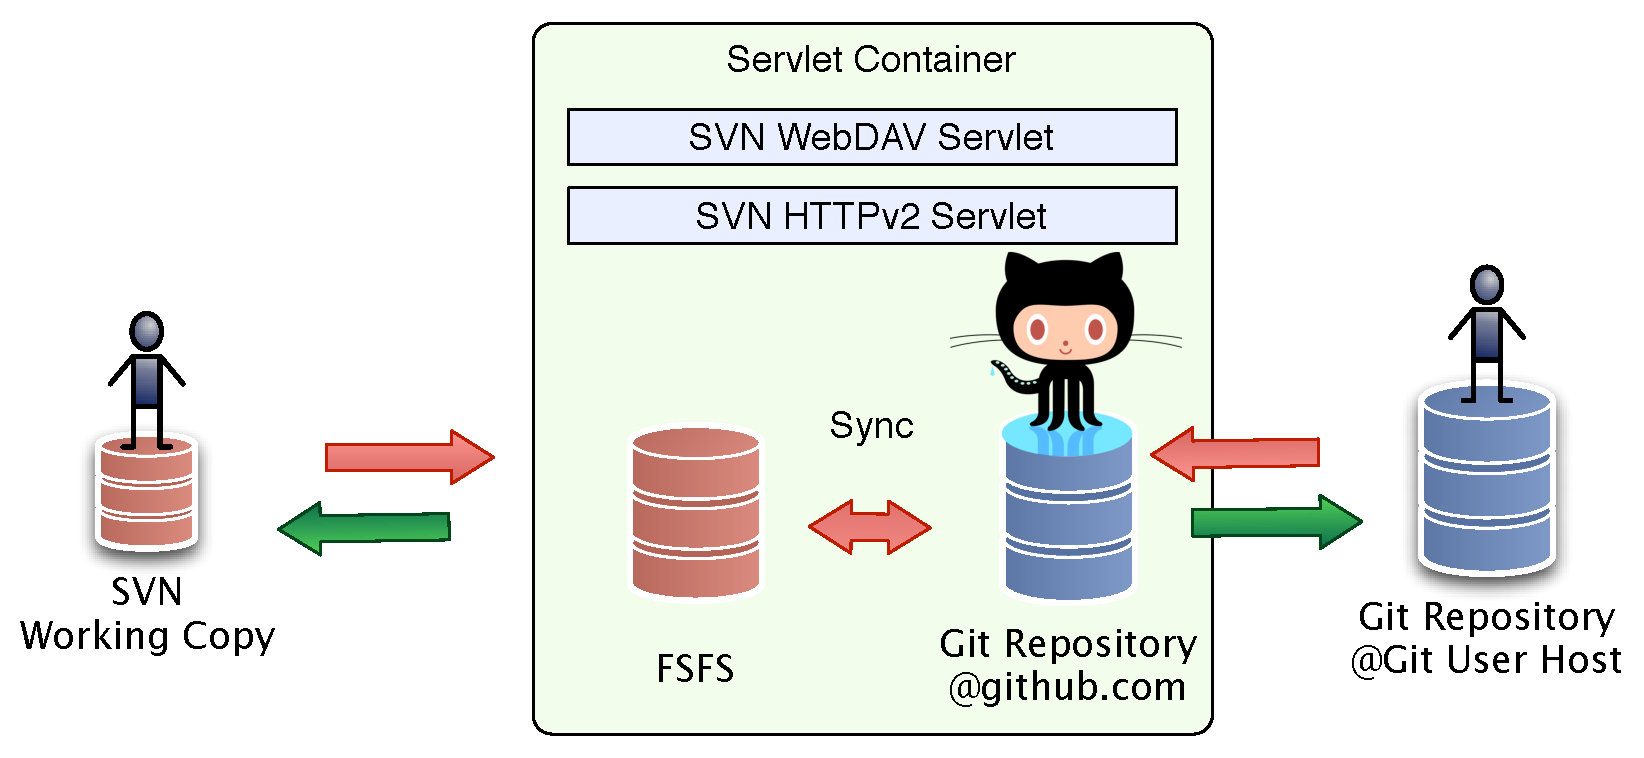
\includegraphics[width=\linewidth]{img/servlet/components_not_that_safe.pdf}
\caption{Architecture.}
\end{figure}

You may use \ref{arch} as a reference to a picture.

\end{document}